\documentclass[twoside,openright,titlepage,headings,footinclude=true,cleardoublepage=empty,BCOR=5mm,11pt,a4paper,english]{book}

\PassOptionsToPackage{utf8}{inputenc}
 \usepackage{inputenc}

\PassOptionsToPackage{T1}{fontenc} 
 \usepackage{fontenc}

\PassOptionsToPackage{english}{babel}
 \usepackage{babel}

\PassOptionsToPackage{autostyle}{csquotes}
 \usepackage{csquotes}

\PassOptionsToPackage{english}{varioref}
 \usepackage{varioref}

\PassOptionsToPackage{fleqn}{amsmath}
 \usepackage{amsmath}

\usepackage{siunitx,amssymb,braket,mhchem}
\sisetup{separate-uncertainty=true, multi-part-units = single}

\usepackage[dvipsnames]{xcolor}%colors più fighi
\definecolor{halfgray}{gray}{0.55}

\usepackage{geometry,appendix}

\usepackage{tabularx} % better tables
	\setlength{\extrarowheight}{3pt} % increase table row height

\usepackage{caption}
\captionsetup{format=hang,font=small,labelfont={sf,bf}}

\usepackage{subfig,multirow,booktabs}

\usepackage{bm}

\usepackage{wrapfig}

\pdfcompresslevel=9
\pdfadjustspacing=1 
\PassOptionsToPackage{pdftex}{graphicx}
	\usepackage{graphicx}
	
\usepackage{comment}

\PassOptionsToPackage{bibstyle=numeric,citestyle=numeric-comp,backend=bibtex,sorting=none}{biblatex}
 \usepackage{biblatex}
\addbibresource{bibliography.bib}

\usepackage{chemformula}


\begin{document}

\begin{titlepage}
\vspace{5mm}
\begin{figure}[hbtp]
\centering

\includegraphics[scale=.13]{Images/UnipdLogo.png}
\end{figure}
\vspace{5mm}
\begin{center}
{{\huge{\textsc{\bf UNIVERSIT\`A DEGLI STUDI DI PADOVA}}}\\}
\vspace{5mm}
{\Large{\bf Dipartimento di Fisica e Astronomia ``Galileo Galilei''}} \\
\vspace{5mm}
{\Large{\textsc{\bf Corso di Laurea Magistrale in Fisica}}}\\
\vspace{15mm}
{\Large{\textsc{\bf Tesi di Laurea}}}\\
\vspace{15mm}
\begin{spacing}{3}
{\LARGE \textbf{Sviluppo e caratterizzazione di una sorgente di plasma a pressione atmosferica per la coagulazione non termica del sangue​}}\\
\end{spacing}
\vspace{5mm}
\end{center}

\vspace{10mm}
\begin{spacing}{1.5}
\begin{tabular}{ l  c  c c c  cc c c c c  l }
{\Large{\bf Relatore}} &&&&&&&&&&& {\Large{\bf Laureando}}\\
{\Large{\bf Prof. Emilio Martines}} &&&&&&&&&&& {\Large{\bf Davide Mancini}}\\
{\Large{\bf Correlatore}}\\
{\Large{\bf Dr. Gianluca De Masi}}\\
{\Large{\bf Dr. Luigi Cordaro}}\\
\end{tabular}
\end{spacing}
\vspace{10 mm}

\begin{center}
{\Large{\bf Anno Accademico 2018/2019}}
\end{center}
\end{titlepage}
\clearpage{\pagestyle{empty}\cleardoublepage}


\tableofcontents

\pagestyle{headings}


\chapter{Introduction}
\label{ch:intro}
Plasma medicine is an emerging field that is broadening its applications from uses on medical equipments (sterilization, decontamination) to uses on living tissues \cite{plmed_review}. One of the reserch groups working in Consorzio RFX laboratories, in Padova, developed a source for the production of Cold Atmospheric Plasma (CAP) to be used for medical treatment on biological tissues: Plasma Coagulation Controller (PCC) \cite{DeMasi_2018}. The source is a Dielctric Barrier Discharge reactor, where a dielectric is used to produce plasma with low charge density. It is developed to promote non thermal blood coagulation, i.e. acceleration of blood clot formation thanks to plasma direct application.

CAPs are of particular interest in plasma medicine for two characteristics:
\begin{itemize}
 \item \textbf{Cold plasma} : given non thermal equilibrium and ion low temperature, this plasma can be applied on surfaces without a dangerous increase in target temperature. In plasma medicine CAPs allow treatment on living tissues, where target temperature must be kept below a safe value.
 \item \textbf{Reactive Species} : When a gas is ionized at atmospheric pressure, the produced plasma is mixed with the surroundig air molecules. The peculiarity of a plasma in air is the presence of reactive species, ions, produced by ionization and recombination of nitrogen, oxygen, water and other atoms or molecules. There are several biological processes where activation and reactions speed is thought to be related to concentration of Reactive Oxydant Species (ROS) and Reactive Nitrogen Species (RNS) \cite{doi:10.1152/ajplung.2000.279.6.L1005}, \cite{doi:10.1152/ajpcell.00366.2006}. 
\end{itemize}

In this chapter there is the presentation of some results obtained with PCC and a general description of the production of CAP, describing the sources developed at Consorzio RFX.

\section{Plasma medicine}
The most studied therapeutic effects of plasma application are:
\begin{itemize}
 \item sterilization and decontamination \cite{Martines_2009}, \cite{Stoffels_2007};
 \item blood coagulation \cite{Fridman2006};
 \item wound disinfection and healing \cite{Haertel2014};
 \item cancer cell treatment \cite{Yan2016}.
\end{itemize}
How plasma interacts with living tissues and produces those effects is not fully understood. Reactive species, along with UV radiation and electromagnetic field, are considered fundamental partecipants of the mechanism.

Previous works studied PCC induced bactericidal effects and non thermal blood coagulation; in the following their results will be described briefly.

\paragraph{Bactericidal effects}
There are numerous studies on the effects of CAPs on bacteria \cite{1167632}, \cite{1673530}, however mechanisms leading to inactivation of bacteria are not fully understood. It is tought that plasma application has an effect when reactive species, UV photons and charged particles comes into direct contact with cell's membrane and structures \cite{plmed_review}.

In figure \ref{fig:bact} is presented the reduction of bacteria vitality due to application of plasma produced with our sources. From the figure it's possible to see results of the experiment on three different bacteria species, for an RF source and for the DBD source, PCC, with three different experimental setups. PCC seems to have a faster effect on the reduction of bacteria, for all analyzed species. 
\begin{figure}
 \centering
 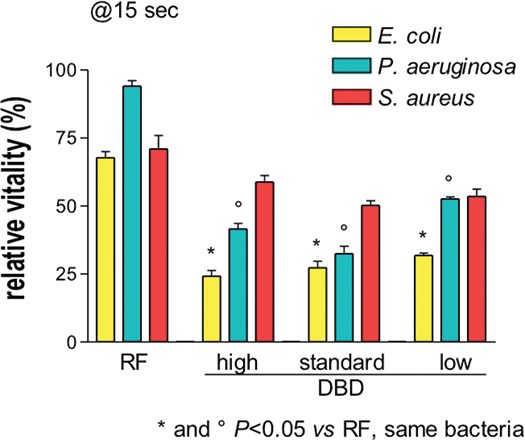
\includegraphics[width=0.5\textwidth]{Images/Intro/bacteria2.png}
 \caption{Relative vitality on different bacteria colonies after plasma treatment of \SI{15}{\second} with different sources. On the left there is treatment with an RF plasma source; on the right there is treatment with the DBD plasma source studied in this work, PCC, for three different combinations of parameters for the discharge (low, standard and high).}
 \label{fig:bact}
\end{figure}


\paragraph{Blood coagulation}
Cauterization devices that produce quasi-thermal blood coagulation with high-temperature plasma have been used for a long time in wound treatment and surgery. Only recently studies shown that with cold plasma application is possible to induce natural blood coagulation, without temperature increase \cite{Fridman2006}, \cite{4343167}.
Treatments with CAPs activate the coagulation cascade shown in figure \ref{fig:coag}, a chain of reactions that involves many tissue factors and proteins. The exact mechanisms that accelerates clot formation have to be understood yet, as of today studies show that plasma induces the production of fibrin that catalyses blood coagulation factors \cite{plmed_review}.
\begin{figure}
 \centering
 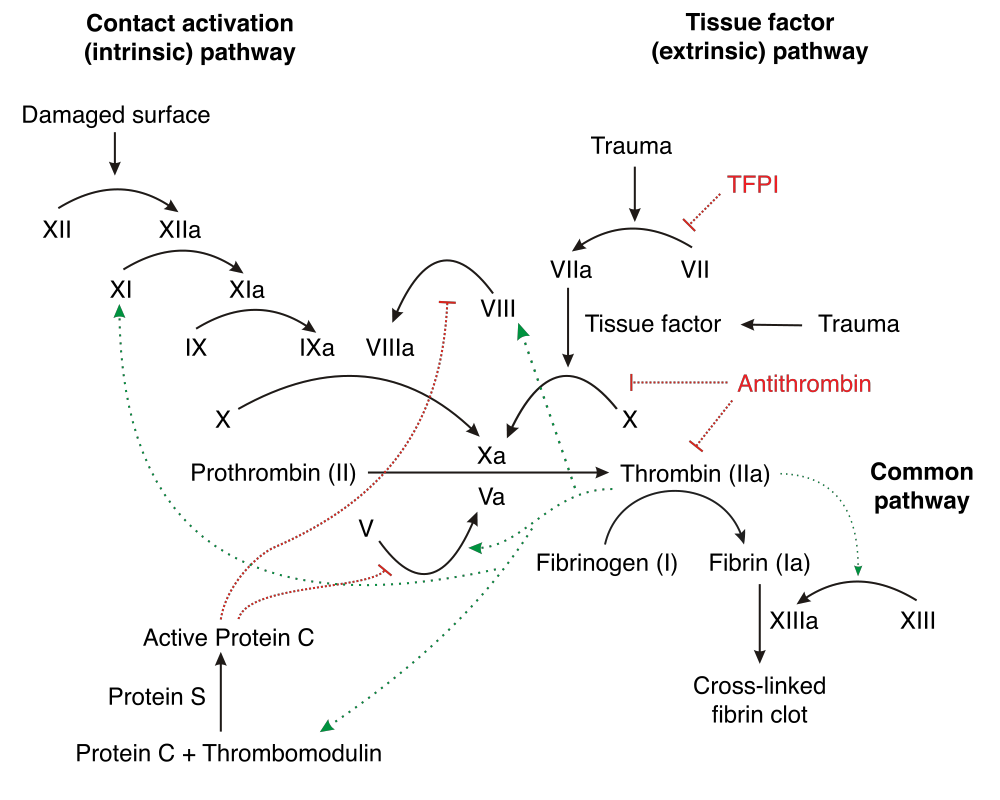
\includegraphics[width=0.8\textwidth]{Images/Intro/coag_map.png}
 \caption{Reaction chain that leads to blood coagulation. The analysis of blood samples treated with plasma, allows to find where and how plasma intervenes in this scheme.}
 \label{fig:coag}
\end{figure}


Treatment with PCC is done applying plasma on blood samples, as shown in figure \ref{fig:plasmaapp} (a). The study involves the use of different plasma application times and different discharge parameters. The effect of plasma application is evaluated from samples as those in figure \ref{fig:plasmaapp} (b), where the blood is removed and the area of the remaining coagulated blood is measured, leading to results in figure \ref{fig:plasmaapp} (c). Results show always an increase on blood coagulation when treated with plasma. 
\begin{figure}
 \centering
 \subfloat[Picture of plasma application.] {
    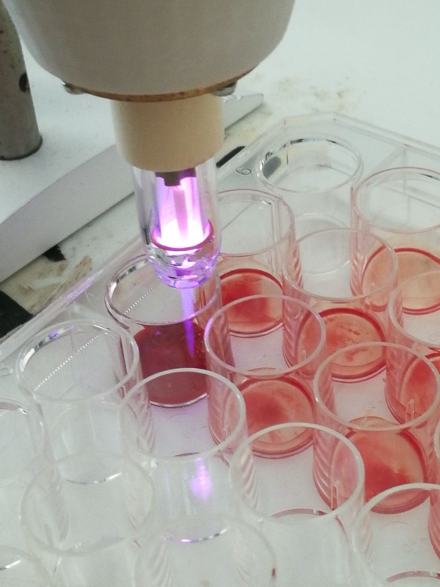
\includegraphics[width=0.4\textwidth]{Images/Intro/source_application.png}
 }
 \hfill
 \subfloat[Coagulated blood samples.]{
    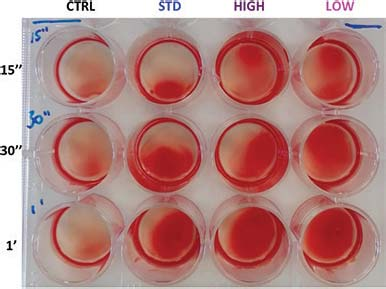
\includegraphics[width=0.5\textwidth]{Images/Intro/blood_sample.png}
 }
 \vspace{1cm}
 \subfloat[Coagulated blood area.]{
    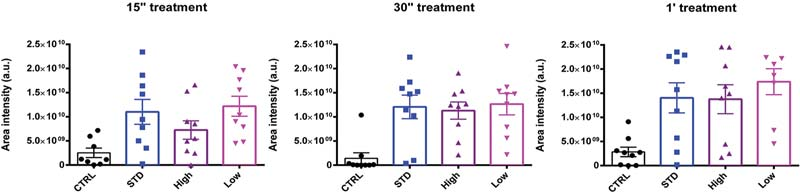
\includegraphics[width=\textwidth]{Images/Intro/coag_histo.png}
 }
 \caption{Pictures and results of the blood coagulation study with PCC. Blood samples are treated with three different parameters of the DBD discharge, for three different application times. In (c) is possible to see the increse of coagulated blood area for samples treated by plasma, if compared to the control sample.}
 \label{fig:plasmaapp}
\end{figure}


\begin{comment}
\paragraph{ROS and RNOS presence}

\begin{figure}
 \centering
 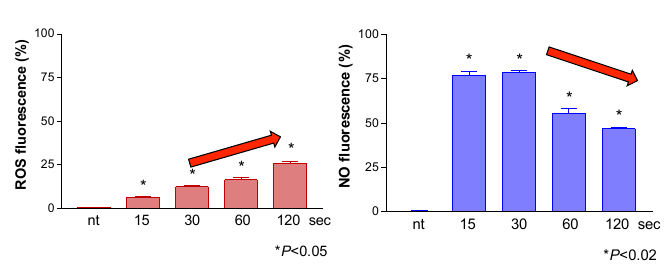
\includegraphics[width=0.4\textwidth]{Images/Intro/ROS.png}
 \caption{ROS and NO fluorescence }
 \label{fig:ROS}
\end{figure}
\end{comment}


\section{Cold Atmospheric Plasma}
In a CAP thermodynamical equilibrium is not reached. Electron energy is usually much higher than ion energy \cite{VONENGEL196599}. In those conditions plasma dynamics can be described as the collective motion of two interpenetrating fluids, where the thermal motion of ions can be ignored \cite{goossens2012introduction}.
There are several studies on CAP plasma characteristics \cite{Zhu_2009}, \cite{Ohyama_2009}, \cite{Amorim_2015} typical values are electron temperatures between $T_e = 1 - \SI{10}{\electronvolt}$ and electron densities between $n_e = \num{e17} - \SI{e22}{\meter^{-3}}$ , inside the box outlined in figure \ref{fig:plasmaclass}. 
\begin{figure}
 \centering
 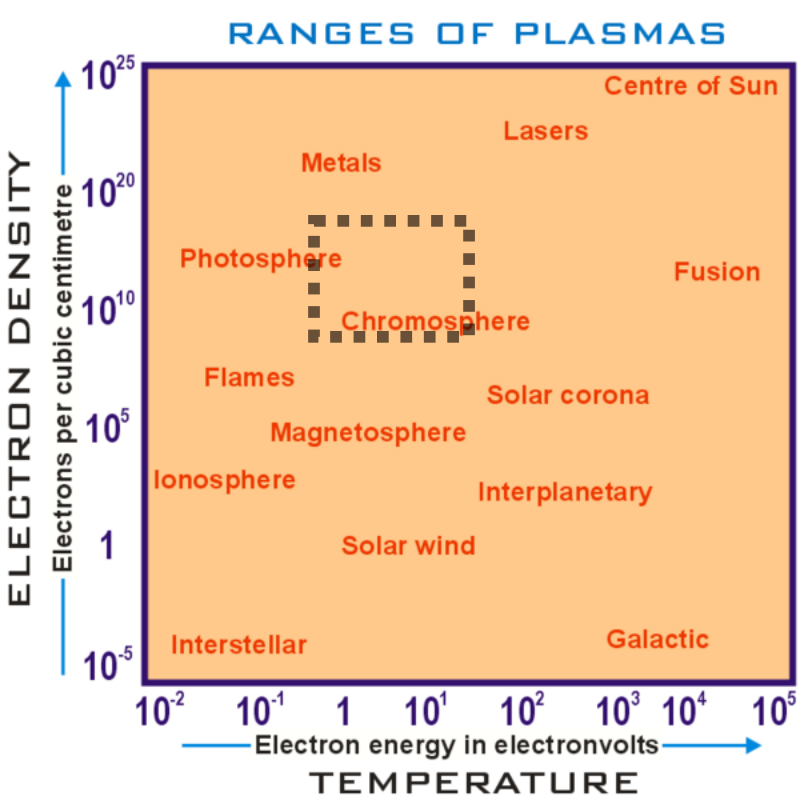
\includegraphics[width=0.5\textwidth]{Images/Intro/Plasma_classification2.png}
 \caption{Plasma classification in function of electron density and electron temperature. Inside the square there are typical parameters for CAPs.}
 \label{fig:plasmaclass}
\end{figure}


\subsection{Plasma generation}
Electron density in CAPs is much smaller than the neutral density of an ideal gas $n_{n} = \SI{2.50e25}{\meter^{-3}}$. However it is higher than the density of free electrons naturally present in air at atmospheric pressure. Radioactive substances and cosmic rays generates electron-ion pairs with a total ionization rate of $\SI{e7}{\meter^{-3}\second^{-1}}$ \cite{book:1593058}.

The application of a steady electric field to a gas accelerate free electrons that collide with atoms and molecules resulting in excitation or ionization reactions. If the electric field has enough intensity it extract electrons from atoms and molecules ionizing them. Those reactions form ion-electron pairs that are accelerated producing other pairs, inducing chain reactions that could sustain plasma discharge. If and how this process starts is influenced by:
\begin{itemize}
 \item gas species, by their ionization potential and cross section for different reactions
 \item characteristics lenght of the system, that influences charged particle's acceleration
 \item gas pressure, that is proportional to reaction rates
\end{itemize}
%The breakdown conditions are defined by the well known Paschen curves, where the voltage breakdown potential is studyed for different values of the product of electrodes distance and gas pressure, related respectively to electron acceleration and collisions frequency.

Generally electrons acquire more energy from the electric field due to the lower mass and higher mobility, so electronic temperature increases more rapidly then ion temperature. If we apply a steady DC electric fields, electrons and ions reach thermal equilibrium trough collisions, generating thermal plasma at high temperatures. To avoid thermalization and produce cold plasma at high densities is possible to give energy selectively to electrons with AC electric fields at high frequency \cite{BARDOS20106705}.


Two examples of sources that produce plasma for medical application are the ones built at RFX: the RF source based on a radio transmitter (\cite{Martines_2009}) and the DBD source, studied in this work (\cite{DeMasi_2018}).

\paragraph{RF source}
The RF source developed in RFX works applying an AC electric field between two electrodes. It is composed by two coaxial tubes as shown in figure \ref{fig:RF}: the internal one is connected to a radio transmitter in series with a matching network and with an electrode formed by a wire grid; the external one ends with a second electrode fixed at ground potential. The radio transmitter works with fixed power (\SI{5}{\watt}) and is set to a specific frequency that is the resonance frequency for the LC series circuit formed by the induttance in the matching network and the parasitic capacitance of the device. When neutral gas flows inside the inner tube, the electric field between the electrodes ionizes it, producing cold plasma in air. The source is built with an induttance of \SI{100}{\micro\henry}, capacitance is estimated as \SI{10}{\pico\farad}, resulting in a resonance for a frequency around \SI{4.8}{\mega\hertz}, reaching voltage peak to peak values up to \SI{900}{\volt} on the electrode. By setting an appropriate gas flow, the discharge starts more easily and to reach lower peak voltage values.
This source produces plasma directly in air, so it ionizes a mixture of neutral gas and air, giving birth to plasma rich in reactive species coming from oxygen and nitrogen molecules. The presence of reactive species allows to use this source for non-thermal sterilization of living tissues: plasma produced by it has bactericidal effects and does not damage human cells (\cite{doi:10.1002/ppap.200700154}).
\begin{figure}
 \centering
 \subfloat[Source scheme.]{
    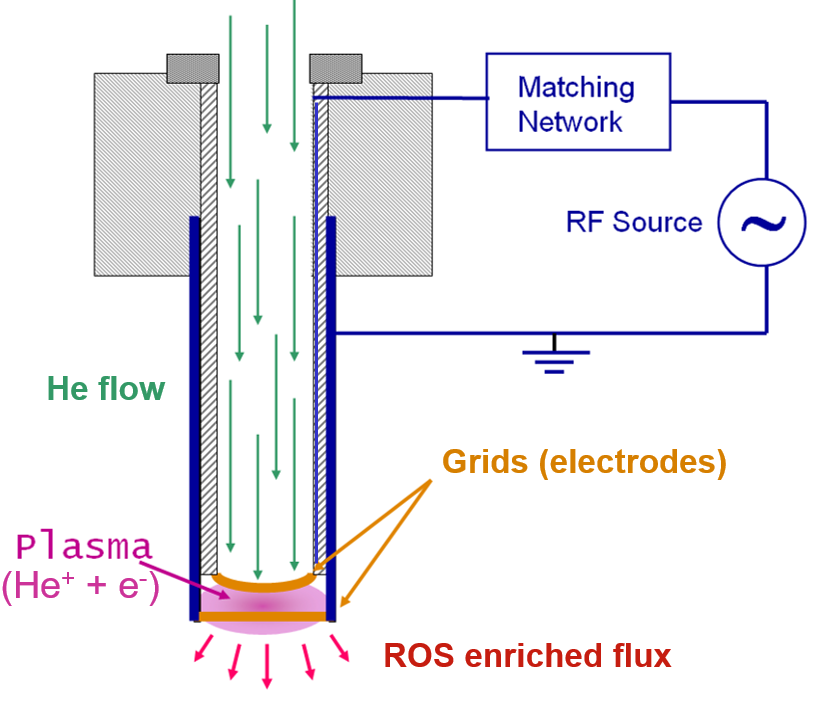
\includegraphics[width=0.4\textwidth]{Images/Intro/RF.png}
 }
 \hfill
 \subfloat[Picture of produced plasma.]{
    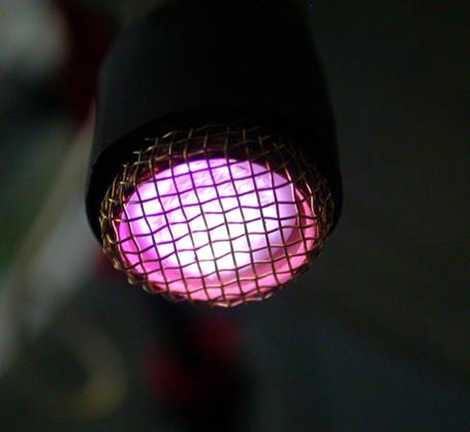
\includegraphics[width=0.4\textwidth]{Images/Intro/RF_plasma.png}
 }
 \caption{Plasma RF source developed in RFX.}
 \label{fig:RF}
\end{figure}


\paragraph{DBD source}
The source developed in this work is based on the Dielectric Barrier Discharge (DBD): it applies an electric field on the gas with one electrode or a pair of electrodes, where a dielectric covers at least one of them, as in figure \ref{fig:DBDex}.
The dielectric works as an insulator and does not allow DC current to flow in the gap, so gas between the electrodes can be ionized without large current densities flowing trough the resulting plasma (\cite{Kogelschatz2003}). The discharge can be modelized as in the circuit in figure \ref{fig:DBDex} (b) (\cite{DBDcircuit}), $C_1$ is capacitance of dielectric, $C_2$ of air and $R_p$ and $C_p$ are plasma resistance and capacitance (in other studies it is possible to find more refined models \cite{doi:10.1063/1.4986023}). Typical values for discharge parameters are AC voltage frequency or pulse rates $f \ge \SI{1}{\kilo\hertz}$, voltage peak values from $V_{p} = 1 - \SI{20}{\kilo\volt}$, and current peak intensities on a conductive target $I < \SI{100}{\milli\ampere}$.
\begin{figure}
 \centering
 \subfloat[DBD scheme with two electrodes.]{
    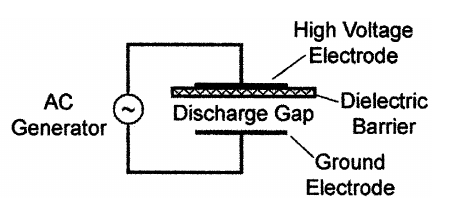
\includegraphics[width=0.48\textwidth]{Images/Intro/DBD_es1.png}
 }
 \hfill
 \subfloat[DBD circuit diagram.]{
    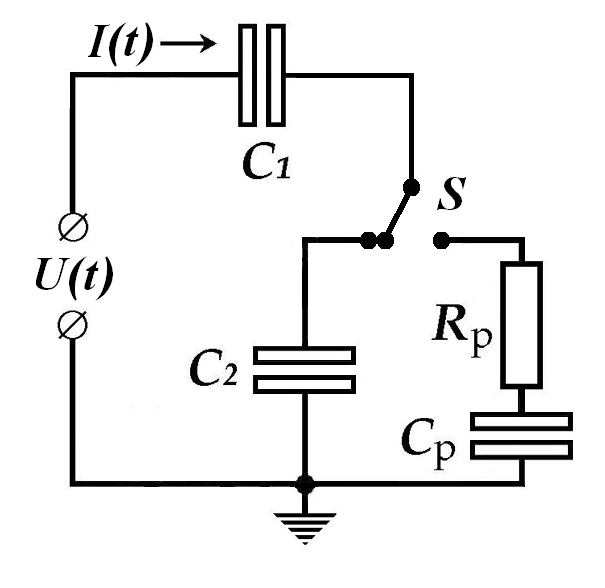
\includegraphics[width=0.4\textwidth]{Images/Intro/Fig1DBD.png}
 }
 \caption{Representation of the concept behind DBD plasma production: on the left  an experimental setup composed by two electrodes, one dielectric and a voltage AC generator; on the right a circuit diagram of the setup for DBD discharge. In the circuit, $C_1$ is the dielectric capacitance, $C_2$ the air capacitance, $C_p$ and $R_p$ are plasma capacitance and resistance.}
 \label{fig:DBDex}
\end{figure}

DBD plasma reactors changed in the last decades following the development of pulse power technology: from the classic sinusoidal voltage now is common to apply pulsed voltage. Plasma generated with sub-microseconds voltage pulses allows to avoid local discharges overheat and increases discharge production of reactive species inside the plasma (\cite{SHAO2009215}). Those progresses in DBD plasma technology led to the development of sources for biomedical plasma applications. Those plasma sources, including PCC, have to produce plasma rich in reactive species, while meeting stringent requirements such as low temperature (at or near room temperature), no risk of arcing, operation at atmospheric pressure, preferably hand-held operation, low concentration of ozone generation, etc.

The design used in many works is in figure \ref{fig:DBDmed} (\cite{Stoffels_2006}, \cite{doi:10.1063/1.2045549}): a cylindrical electrode is covered in dielectric material and inserted in a tube with neutral gas flowing in it. The gas, typically helium or argon, allows to start plasma discharge, then plasma is expelled in air where it produces reactive species needed for medical treatment. PCC developed and studied in this thesis will be described in details in chapter \ref{ch:electric}, along with its electrical characterization.
\begin{figure}
 \centering
 \subfloat[\emph{Plasma pencil} \cite{Stoffels_2006}.]{
    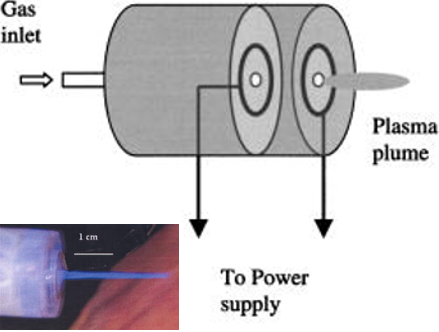
\includegraphics[width=0.4\textwidth]{Images/Intro/DBDmed5.png}
 }
 \hfill
 \subfloat[\emph{Plasma needle} \cite{doi:10.1063/1.2045549}.]{
    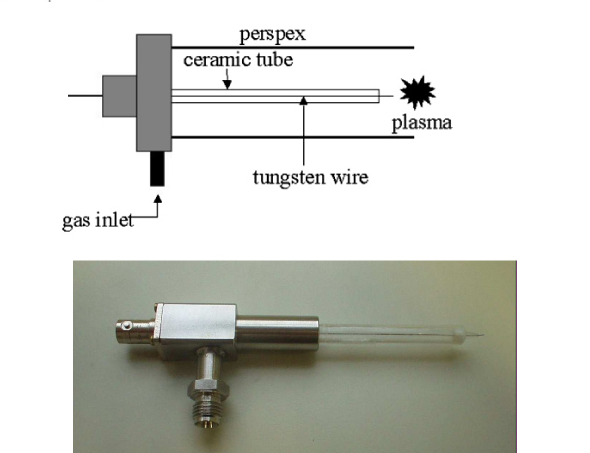
\includegraphics[width=0.4\textwidth]{Images/Intro/DBDmed4.png}
 }
 \caption{Two example of DBD plasma sources for medical applications. In both sources we have one electrode that applies an electric field to neutral gas, ionizing it. Plasma is then expelled in air at atmospheric pressure.}
 \label{fig:DBDmed}
\end{figure}


An intersting phenomenon in sources with this design is plasma formation and propagation. High speed camera measuraments of the process show that plasma is not produced in a uniform steady column, but every pulse of the electric field gives start to localized plasma emission. Once produced, the ionization wave moves from the electrode and propagates in air, with velocities from \num{10} to over \SI{150}{\kilo\meter/\second}. Those localized plasma emissions are called ``bullet'' and only recently is possible to find models that describe them \cite{Lu2016DynamicsOA}.
In this thesis this phenomenon is observed and sudied in details in chapter \ref{ch:shape}, with different voltage pulse parameters, target position and gas composition.


As said before, the purpose of non thermal plasma application for medical uses is the deposition of reactive species on biological tissues. The presence and chracteristics of reactive species can be studied by emission spectroscopy, with intensity and temperature estimation. Chapter \ref{ch:spectrometry} is dedicated to the study of plasma radiation emission around visible wavelengths.


The other fundamental feature of plasma produced by our source is that can be applied on human body without danger. Temperature measurements on the target of plasma application can lead to an estimation of plasma power deposition. In chapter \ref{ch:temperature} are presented thermocamera mesurements and power estimation.

\clearpage
\chapter{Electric characterization}
\label{ch:electric} 
The development of electric components used to produce the Plasma Coagulation Controller is highly influenced by the need of flexibility in settings and mobility for wound treatment. To produce plasma as DBD, in air with Helium or Argon as ignition gasses, it is necessary to produce high voltage, to permit easy medical application the design of the head must be compact with particular attention to electric safety measuraments.
The scheme outputs a voltage pulse with an amplitude up to $\SI{10}{\kilo\volt}$ and frequencies up to $\SI{50}{\kilo\hertz}$.

A rappresentation of power and signal line is in figure \ref{fig:electricline}. The circuit is divided mainly in two parts %as described in chapter \ref{ch:source}
: the controller, with alimentation and settings controls, and the head, where the discharge happens and plasma is emitted.
\begin{figure}
 \centering
 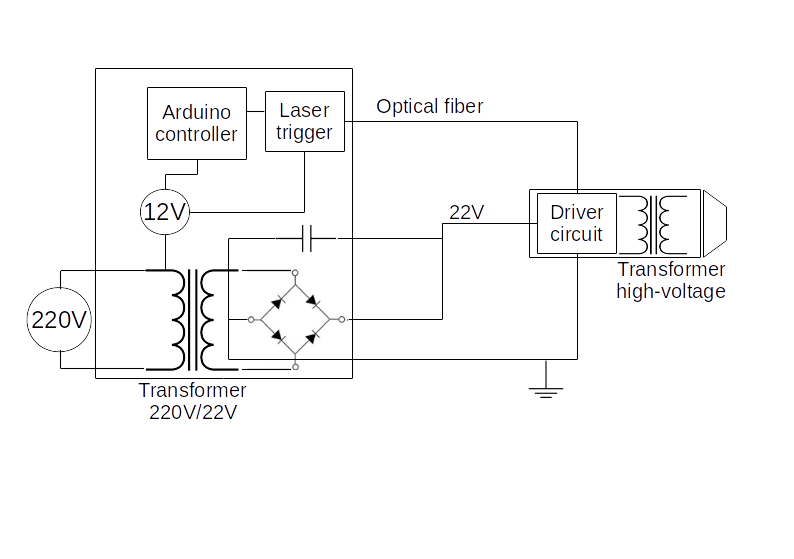
\includegraphics[width=0.8\textwidth]{Images/Linea_elettrica.png}
 \caption{Scheme of the general electric line to produce high voltage, the controller on the left and the head on the left.}
 \label{fig:electricline}
\end{figure}

The line divides in:
\begin{itemize}
 \item \bf{Alimentation} : the $\SI{220}{\volt}$ DC power line goes in a transformer that gives a $\SI{22}{\volt}$ tension to the head, passing through a diode bridge. This tension aliments the driver circuit on the head.
 \item \bf{Arduino and trigger} : the power line is reduced to $\SI{12}{\volt}$ necessaries to aliment an Arduino controller and a laser. From an analogical output of the Arduino a PWM wave goes to the laser trigger, it transmit information on the wave frequency and duration with an optical fiber that ends with a photodiode installed on the driver circuit. Wave frequency is setted by the Arduino, wave duration is setted giving the opengin time of the MOSFET installed on the driver circuit. With this setup the High-Voltage line is entirely decopuled from the controller, in this way there are not serious problems of signal reflection on the power line or the Arduino.
 \item \bf{Head} : the Driver Circuit receives a power line of $\SI{22}{\volt}$ and an optical trigger that defines frequency and duration of the voltage pulse. When the trigger gives the start signal the transformer on the head receives on primary circuit a voltage of hundreds $\si{\volt}$ and outputs from secondary circuit a voltage of thousends $\si{\volt}$. Connected to the ouput there is an electrode inside a capillary tube.
\end{itemize}


A simulation of the different signals, obteined with a simplified scheme with Spice, is in figure \ref{fig:signals}. As in the figure...

The characterization of the electric scheme is made measuring output tension and current with different settings for the pulse.


\begin{comment}
La sorgente di plasma funziona tramite l'applicazione di un'alta differenza di potenziale tra gli elettrodi separati da materiale dielettrico, come descritti nel capitolo \ref{ch:sorgente}. La tensione in ingresso nel circuito  della testa della sorgente vengono amplificati fino a tensioni di alcuni \si{\kilo\volt}. Dall'arduino di controllo è possibile regolare il tempo di apertura del circuito in un range di [$2$-$20$] \si{\micro\second} e la frequenza di lavoro in un range di [$2$-$60$] \si{\kilo\hertz}. I parametri importanti per caratterizzare il funzionamento della sorgente saranno quindi tensione e corrente all'uscita del circuito secondario del trasformatore, al variare dei parametri di funzionamento. Utilizzando una lastra metallica posta a potenziale, è possibile misurare la corrente in un dato range temporale. È inoltre possibile stimare la corrente efficace che attraversa il bersaglio, importante nel valutare gli effetti dell'applicazione del plasma.

\section{Setup delle misure di tensione e corrente}
Si vogliono effettuare misure di tensione della sorgente sia senza immissione di elio, senza formazione della plume di plasma, sia nelle condizioni di funzionamento tipiche, con flusso di elio di $\SI{2}{\liter/\minute}$.
Le tensioni vengono misurate tramite una sonda \emph{...} con attenuazione $\times1000$, le correnti tramite una sonda \emph{Tektronix CT2} che per una corrente di \SI{1}{\milli\ampere} restituisce un segnale di \SI{1}{\milli\volt}. I dati vengono letti su un oscilloscopio \emph{Yokogawa DL9040}, che permette il salvataggio dell'intera forma d'onda misurata nei diversi canali. 
Viene effettuata la caratterizzazione elettrica di entrambi i prototipi di sorgente, per i quali il circuito utilizzato è lo stesso, quindi non si aspettano variazioni significative.

\subsection{Misure senza elio}
La sonda ad alta tensione viene collegata all'uscita del circuito secondario, mentre una sonda con attenuazione $\times10$ viene utilizzata per controllare il segnale in ingresso.
La sorgente viene azionata variando la frequenza ($f$) e duty cycle ($\Delta t$). Scelta la frequenza di lavoro, viene variata la duty cycle in un range utile, considerando il tempo necessario al terminare delle oscillazioni del segnale prima dell'arrivo di una nuova onda quadra (per frequenze maggiori si potrà arrivare a duty cycle minori).
Si ottengono curve come in figura \ref{fig:tensione_es}. La risoluzione della misura viene variata in modo da avere l'errore di misura minore possibile.

\begin{figure}
\centering
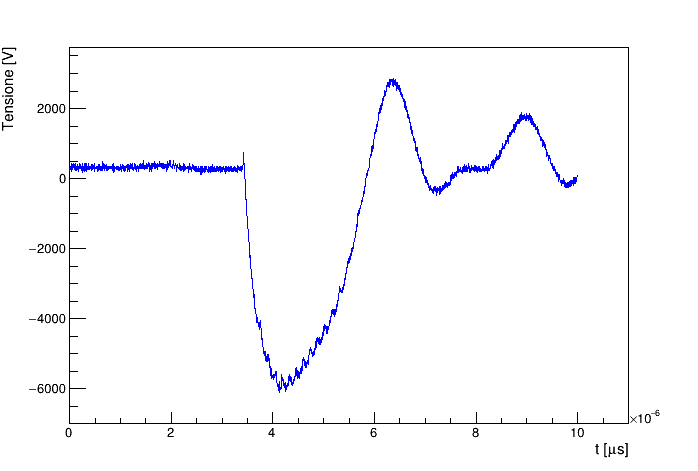
\includegraphics[width=.7\textwidth]{Immagini/tensione_es_2.png}
\caption{Esempio di misura di tensione, $f = \SI{5}{\kilo\hertz}$ e $\Delta t = \SI{16}{\micro\second}$, prototipo 1.}
\label{fig:tensione_es}
\end{figure}

\subsection{Misure con elio}
Per caratterizzare il funzionamento della sorgente nelle possibili condizioni di trattamento, vengono misurate contemporaneamente, su due diversi canali dell'oscilloscopio, tensione alla quale si trova l'elettrodo e corrente che fluisce nel plasma. Per la misura di corrente viene fatto impattare il plasma su una piastra di rame  di dimensioni \SI{2}{\centi\metre} $\times$ \SI{2}{\centi\metre} $\times$ \SI{0.5}{\centi\metre}, ad una distanza di \SI{1}{\centi\metre} dall'elettrodo della sorgente, collegata alla sonda di corrente.
Nuovamente vengono effettuate misure al variare di frequenza ($f$) e duty cycle ($\Delta t$), con le stesse modalità delle misure di tensione.
Tutte le misure sono effettuate con flusso di gas He pari a $\SI{2}{\litre/\minute}$.
Si ottengono curve come in figura \ref{fig:corrente_es}.

\begin{figure}
\centering
 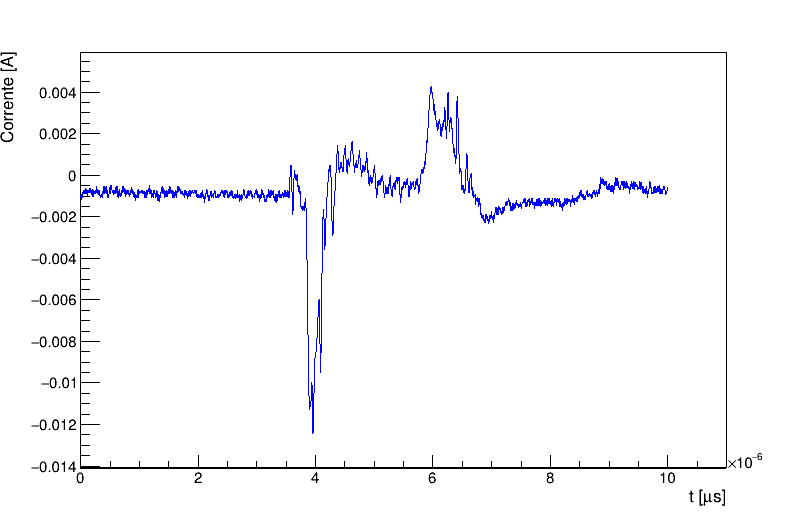
\includegraphics[width=.7\textwidth]{Immagini/corrente_es.png}
\caption{Esempio di misure di corrente per $f = \SI{5}{\kilo\hertz}$ e $\Delta t = \SI{24}{\micro\second}$, prototipo 1.}
\label{fig:corrente_es}
\end{figure}


\section{Presentazione misure ed analisi}
Sia per le misure di tensione che per le misure di corrente si trova un picco negativo come presentato nelle Figure \ref{fig:tensione_es} e \ref{fig:corrente_es}. Il picco di tensione ha valori tipici tra i $\num{3}$ e i $\SI{10}{\kilo\volt}$ in assenza o in presenza di gas, mentre quello di corrente tra i $\num{2}$ e i $\SI{12}{\milli\ampere}$.
L'analisi dei dati prevede la ricerca del massimo della tensione e della corrente nelle diverse configurazioni.

\subsection{Tensione di picco senza elio}
L'andamento medio delle misure presenta un picco negativo pronunciato, compatibile con i tempi di apertura del circuito. Dato un set, il valore di picco viene cercato calcolando la trasformata di Fourier del segnale (tramite le routine fftw3 delle librerie ROOT), tagliando le oscillazioni ad alta frequenza e ricostruendone una media. Nel segnale medio così ricostruito il valore del minimo viene trovato interpolando con una funzione di Landau attorno il minimo, in modo da riprodurre l'asimmetria del picco.
A queste misure viene aggiunto l'errore dovuto al taglio delle alte frequenze, preso come una media del valore assoluto dell'oscillazione del segnale tagliato. Viene inoltre aggiunto l'errore caratteristico dello strumento di misura, trascurabile rispetto l'errore dovuto alle oscillazioni veloci.
In figura \ref{fig:landau} un esempio del fit.

\begin{figure}
\centering
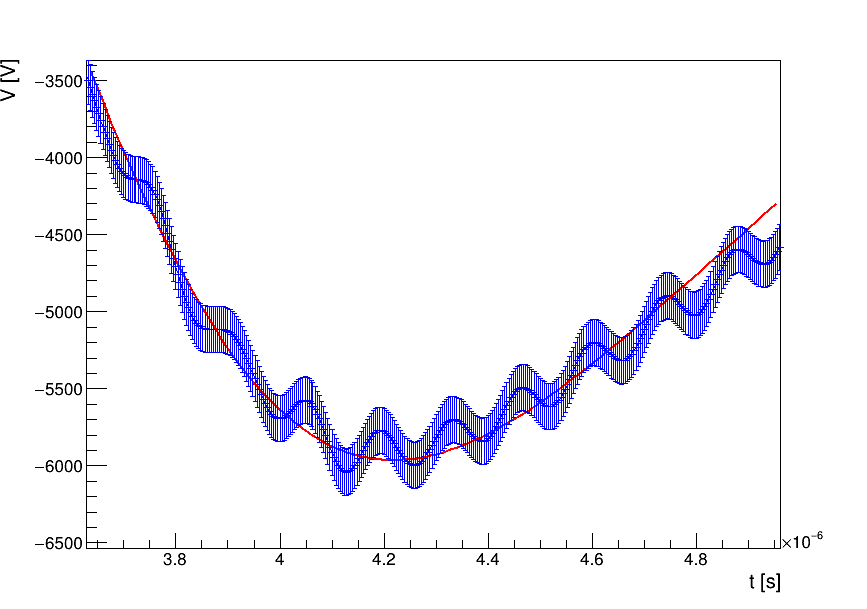
\includegraphics[width=.6\textwidth]{Immagini/esfiterr.png}
\caption{Esempio di fit del picco di tensione, $f = \SI{5}{\kilo\hertz}$ e $\Delta t = \SI{16}{\micro\second}$}
\label{fig:landau}
\end{figure}


Le tensioni del picco così calcolate, al variare della duty cycle per le diverse frequenze, sono presentate in figura \ref{fig:tensioni}.
Per tutte le frequenze di lavoro tra i $\SI{4}{\micro\second}$ e i $\SI{16}{\micro\second}$ risulta un andamento lineare, con tensione variabile tra i $\SI{2}{\kilo\volt}$ e i $\SI{9}{\kilo\volt}$. Aumentando ancora il tempo di apertura del circuito la tensione arriva a valori più elevati, fino un massimo di circa $\SI{10}{\kilo\volt}$, ma viene perso l'andamento lineare.


 \begin{figure}
\centering
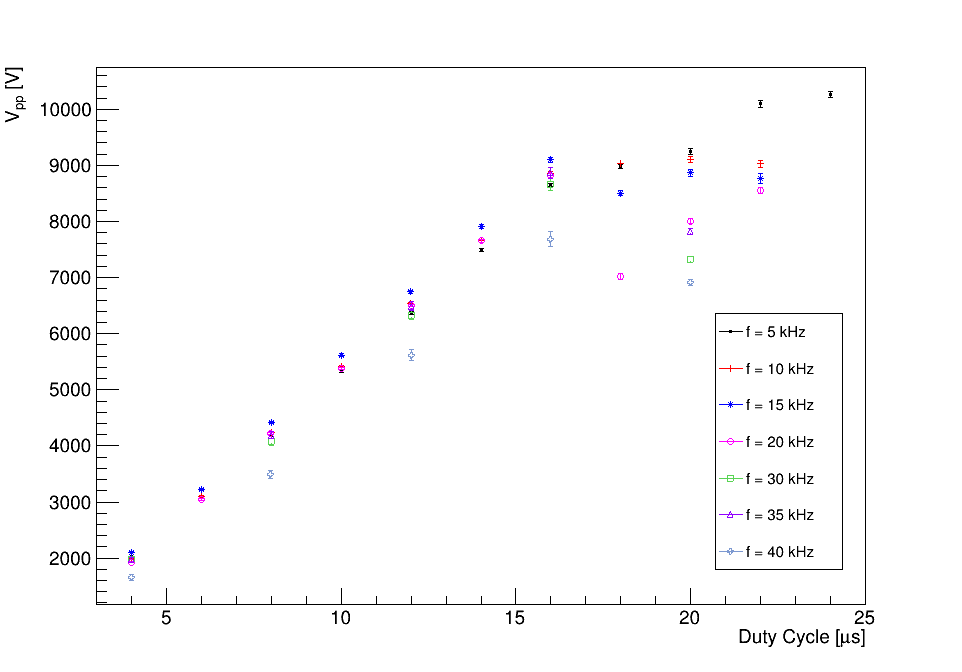
\includegraphics[width=.6\textwidth]{Immagini/nogas.png}
\caption{Tensioni al variare del tempo di apertura del circuito e per diverse frequenze.}
\label{fig:tensioni}
\end{figure}


Le misure non sembrano presentare un andamento in funzione della frequenza, per verificarlo vengono calcolati i coefficenti dell'interpolazione lineare per le varie frequenze, presentati in figura \ref{fig:fitlin}.
Viene confermata l'assenza di un andamento specifico al variare della frequenza.

\begin{figure}
\centering
\subfloat[][Pendenza delle rette.]
  {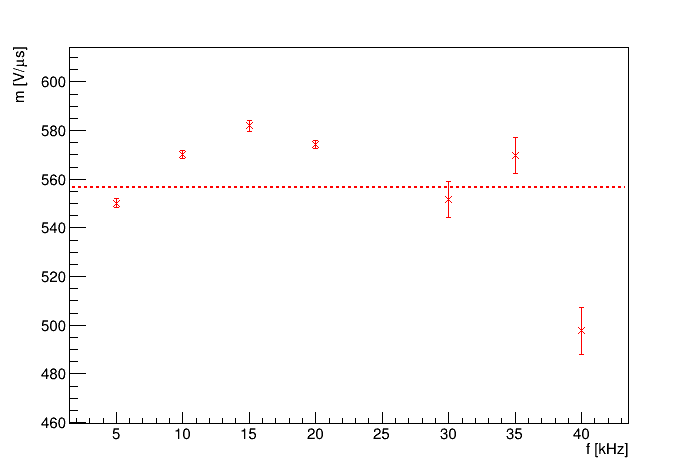
\includegraphics[width=.48\textwidth]{Immagini/m_freq_nogas.png}}
\subfloat[][Intercetta delle rette.]
  {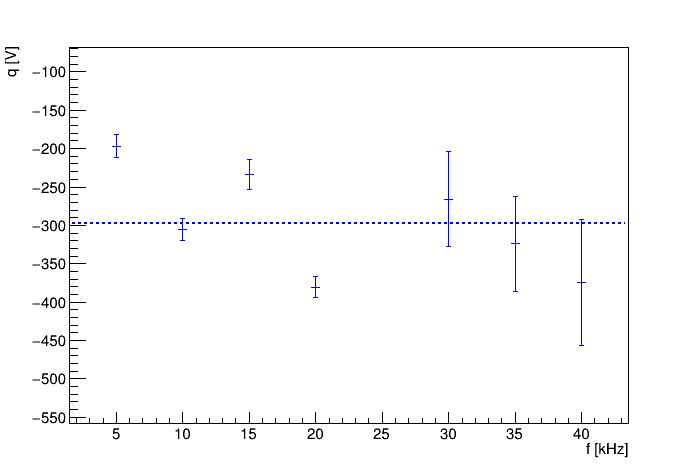
\includegraphics[width=.48\textwidth]{Immagini/q_freq_nogas.png}}
\caption{Parametri dell'interpolazione lineare dei set di misure senza immissione di gas(nel range $\Delta t$ stabilito), al variare della frequenza.}
\label{fig:fitlin}
\end{figure}


\subsection{Tensione e corrente con elio}
Le misure di tensione presentano l'andamento trovato precedentemente, mentre le misure di corrente presentano un primo picco negativo seguito da un picco più basso di segno opposto, positivo. L'analisi proposta è uguale a quella pensata per i set di misure precedenti: vengono tagliate le oscillazioni ad alta frequenza, ricostruito il segnale (aggiungendo l'errore dovuto al taglio delle alte frequenze e agli strumenti di misura) e il valore del minimo viene trovato interpolando con una funzione di Landau. Da questo fit vengono calcolati valori e posizione del picco di tensione, del picco negativo di corrente e del picco positivo di corrente.
In figura \ref{fig:landau} un esempio del fit.

\begin{figure}
\centering
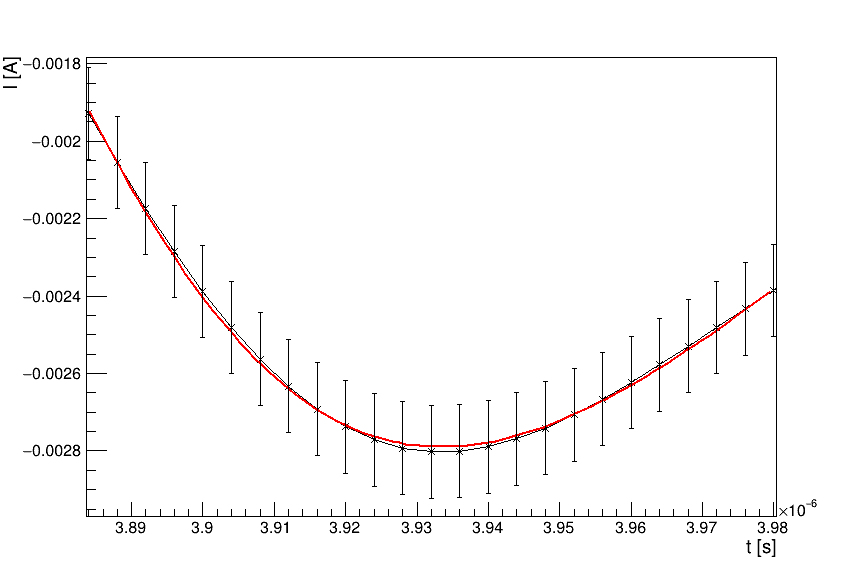
\includegraphics[width=.6\textwidth]{Immagini/es_fit_landau.png}
\caption{Esempio di fit del picco di corrente, $f = \SI{5}{\kilo\hertz}$ e $\Delta t = \SI{24}{\micro\second}$}
\label{fig:landau}
\end{figure}

Le tensioni del picco così calcolate, al variare della duty cycle per le diverse frequenze, sono presentate in figura \ref{fig:picchi}.
Nuovamente troviamo un andamento lineare per la tensione tra i $\num{4}$ e i $\SI{16}{\micro\second}$. Anche il picco negativo di corrente presenta questo andamento lineare, mentre per il picco positivo non è possibile identificare un comportamento simile, i valori si disperdono.

\begin{figure}
\centering
\subfloat[][Modulo del picco di tensione.]
  {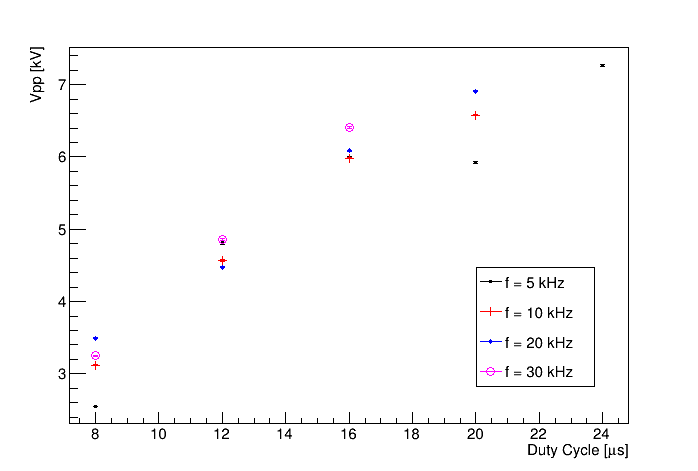
\includegraphics[width=.65\textwidth]{Immagini/vpp_corrente.png}}
\\
\subfloat[][Modulo del picco primario di corrente.]
  {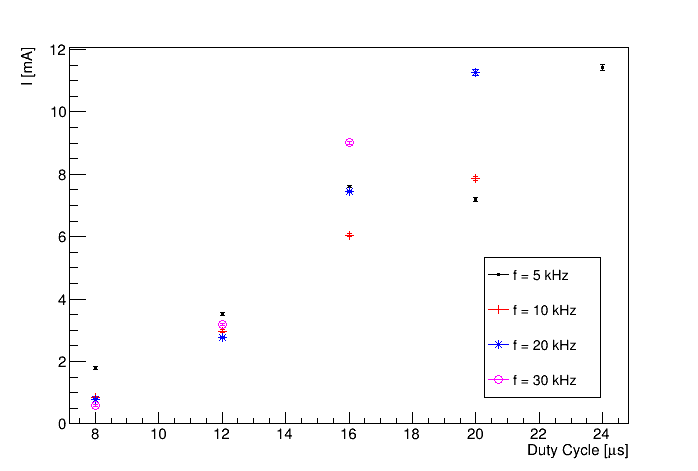
\includegraphics[width=.65\textwidth]{Immagini/I1_corrente.png}}
\\
\subfloat[][Picco secondario di corrente.]
  {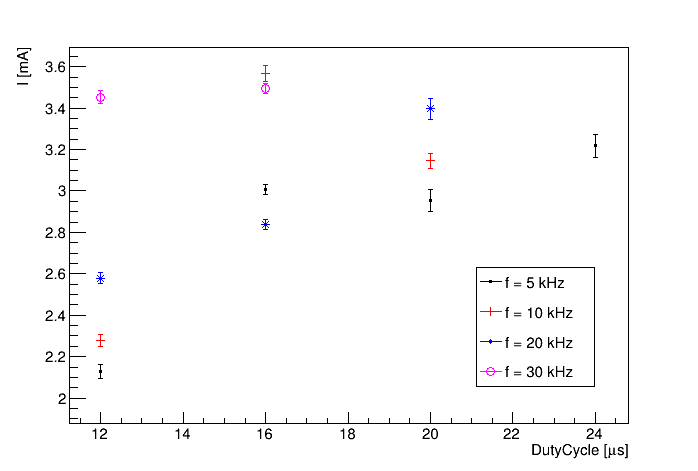
\includegraphics[width=.65\textwidth]{Immagini/I2_corrente.png}}
\caption{Valori dei picchi misurati al variare del tempo di apertura del circuito e per diverse frequenze.}
\label{fig:picchi}
\end{figure}


Nuovamente, per visualizzare in maniera esplicita l'effetto della variazione della frequenza, vengono calcolati i coefficenti dell'interpolazione lineare per le tensioni di picco e per le correnti di picco negativo, presentati in figura \ref{fig:fitlin_cor}. 
Per le tensioni risulta un comportamento identico al precedente, dove i valori si assestano attorno una media lievemente inferiore rispetto le misure in assenza di elio.
Per il valore massimo di corrente viene trovato un aumento in funzione della frequenza di funzionamento della sorgente.

\begin{figure}
\centering
\subfloat[][Pendenze dei picchi di tensione.]
  {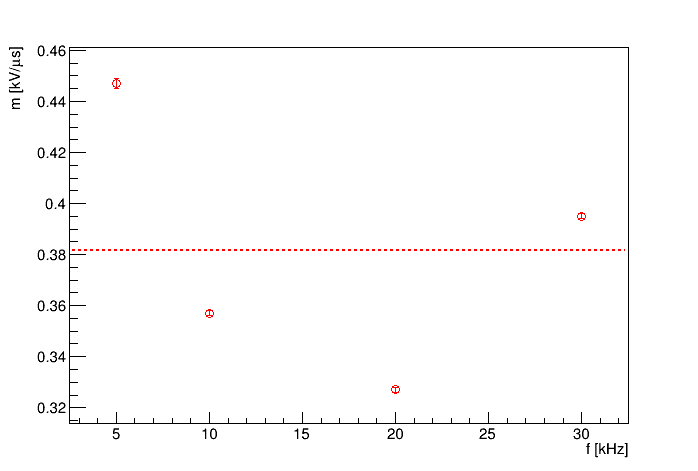
\includegraphics[width=.48\textwidth]{Immagini/mVpp_cor.png}}
\subfloat[][Intercette dei picchi di tensione.]
  {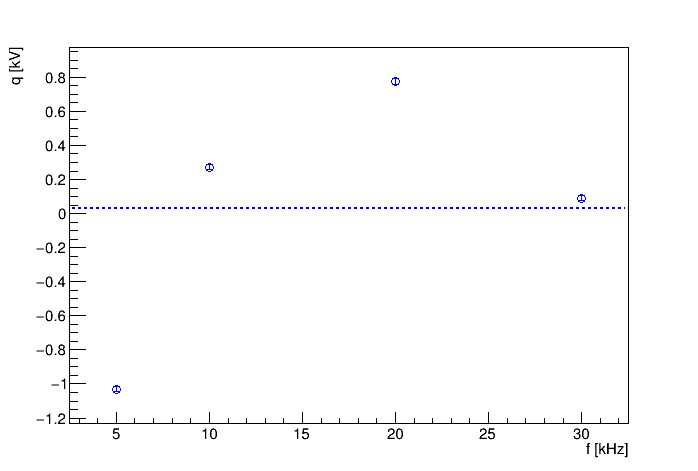
\includegraphics[width=.48\textwidth]{Immagini/qVpp_cor.png}}
\newline
\subfloat[][Pendenze dei picchi di corrente.]
  {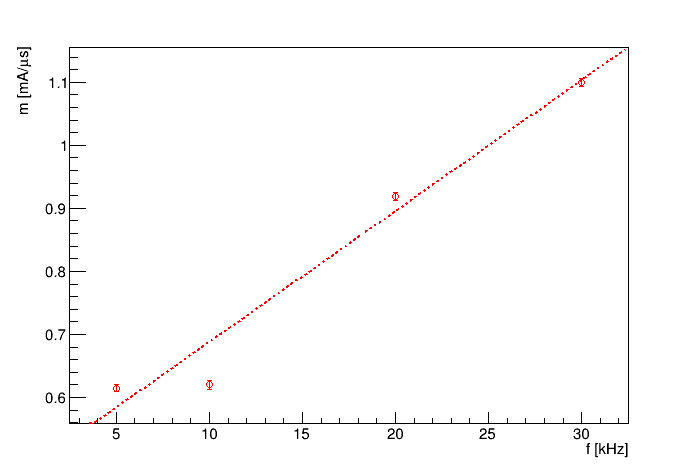
\includegraphics[width=.48\textwidth]{Immagini/mI1_cor.png}}
\subfloat[][Intercette dei picchi di corrente.]
  {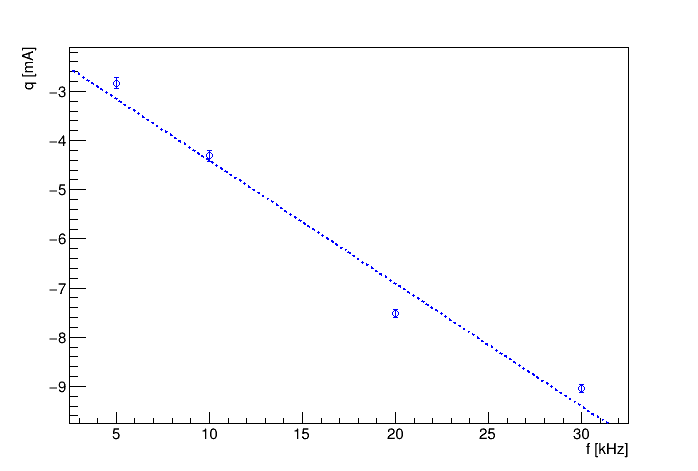
\includegraphics[width=.48\textwidth]{Immagini/qI1_cor.png}}
\caption{Parametri dell'interpolazione lineare dei picchi delle misure di tensione e corrente.}
\label{fig:fitlin_cor}
\end{figure}

\begin{comment}

Data la possibilità di visualizzare contemporaneamente sia la tensione sia la corrente in uscita dal circuito, viene proposta un'analisi delle variazioni temporali tra i diversi picchi. In particolare viene calcolato il tempo tra i due picchi di corrente e tra il picco di tensione e il picco di corrente primario, mostrati in figura \ref{fig:tempi}.
In entrambi i casi non è possibile estrapolare un andamento particolare, indicando che non vi sono differenze significative nei tempi di salita dei picchi al variare del tempo di apertura del circuito e della frequenza.

\begin{figure}
\centering
\subfloat[][Tempo tra i picchi di corrente.]
  {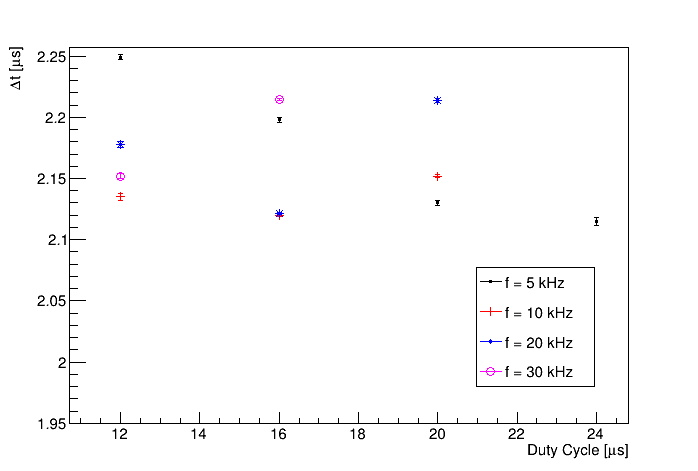
\includegraphics[width=.48\textwidth]{Immagini/ti2ti1.png}}
\subfloat[][Tempo tra picco tensione e primo picco di corrente.]
  {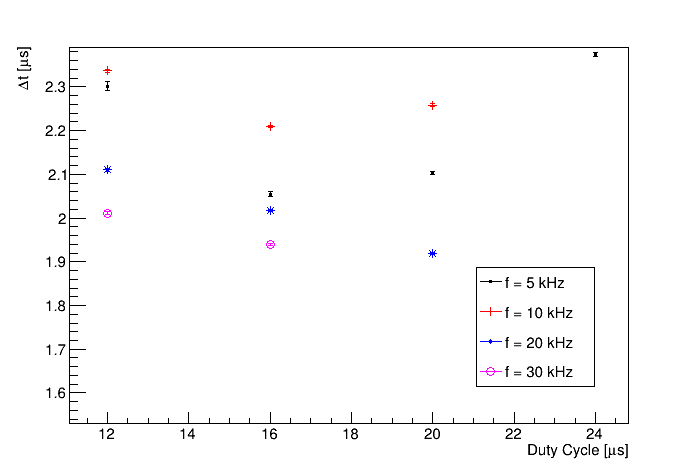
\includegraphics[width=.48\textwidth]{Immagini/ti1tv.png}}
\caption{Misura delle differenze temporali tra i picchi.}
\label{fig:tempi}
\end{figure}

\subsection{Corrente efficace}
Durante l'applicazione del plasma su tessuti vivi bisogna considerare il tempo di reazione effettivo del bersaglio, l'impulso di corrente alle frequenze di lavoro della sorgente presenta un periodo inferiore rispetto questi tempi. Per valutare gli effetti del trattamento viene calcolato il valore della corrente efficace che fluisce sulla piastra bersaglio in un tempo di \SI{1}{\milli\second}, dell'ordine di grandezza dei tempi di risposta da considerare (vedi articolo?), utilizzando la formula in \ref{eq:ieff}.
\begin{equation}
 \centering
 I_{\text{eff}} = \frac{1}{(t_2-t_1)}\sqrt{\int_{t_1}^{t_2} I^2 \,dt}
 \label{eq:ieff}
\end{equation}

In Figura \ref{fig:correff} vengono presentati i valori della corrente efficace in maniera simile a quanto fatto per le misure di corrente precedentemente.
A parità di tempo di apertura del circuito, una maggiore frequenza implica che nel tempo scelto di \SI{1}{\milli\second} vi sarà un numero di periodi maggiore, aumentando la corrente efficace nel circuito. In figura si vede come mediamente la corrente efficace sia più grande a frequenze maggiori, ma assume sempre valori inferiori ai \SI{3}{\milli\ampere}.

\begin{figure}
\centering
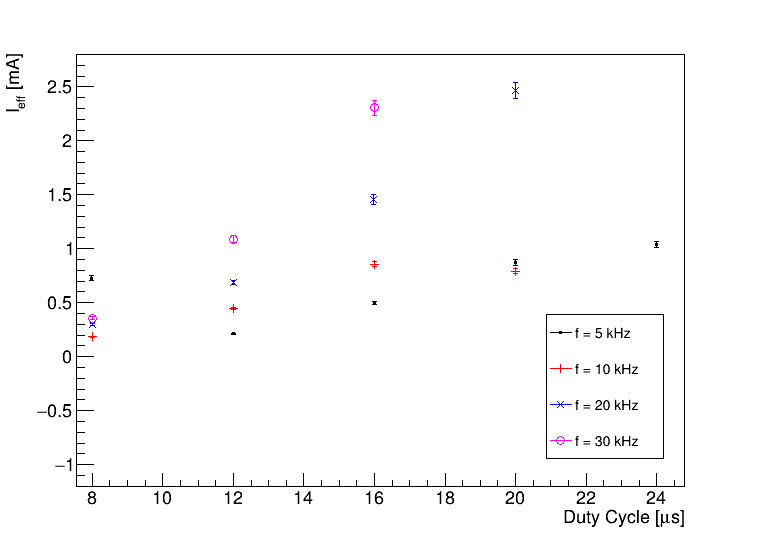
\includegraphics[width=.7\textwidth]{Immagini/ieff.png}
\caption{Corrente efficace calcolata al variare del tempo di apertura del circuito e per diverse frequenze.}
\label{fig:correff}
\end{figure}

\end{comment}

\clearpage
\chapter{Plasma dynamics}
\label{ch:shape}
PCC expels a column shaped plasma plume that emits radiation in a visible range, with different colours and intensity for different gas composition, gas flow and intensity of electric field. In figure \ref{fig:pl_picture} there are pictures of plasma plume with different gas used to start the discharge.

Recent studies shows that what is expelled is not a continuos flow, but the plume is formed by compact collections of emitting particles called \emph{bullets}. Those bullets forms in coincidence of voltage pulses and propagates in air with velocities from \num{10} to over \SI{150}{\kilo\meter/\second} (\cite{Mericam_Bourdet_2009}, \cite{doi:10.1002/ppap.200900078}).

An example of this phenomenon measured with the experimental apparatus used in thesis is shown in figure \ref{fig:pl_bullet}.
\begin{figure}
 \centering
 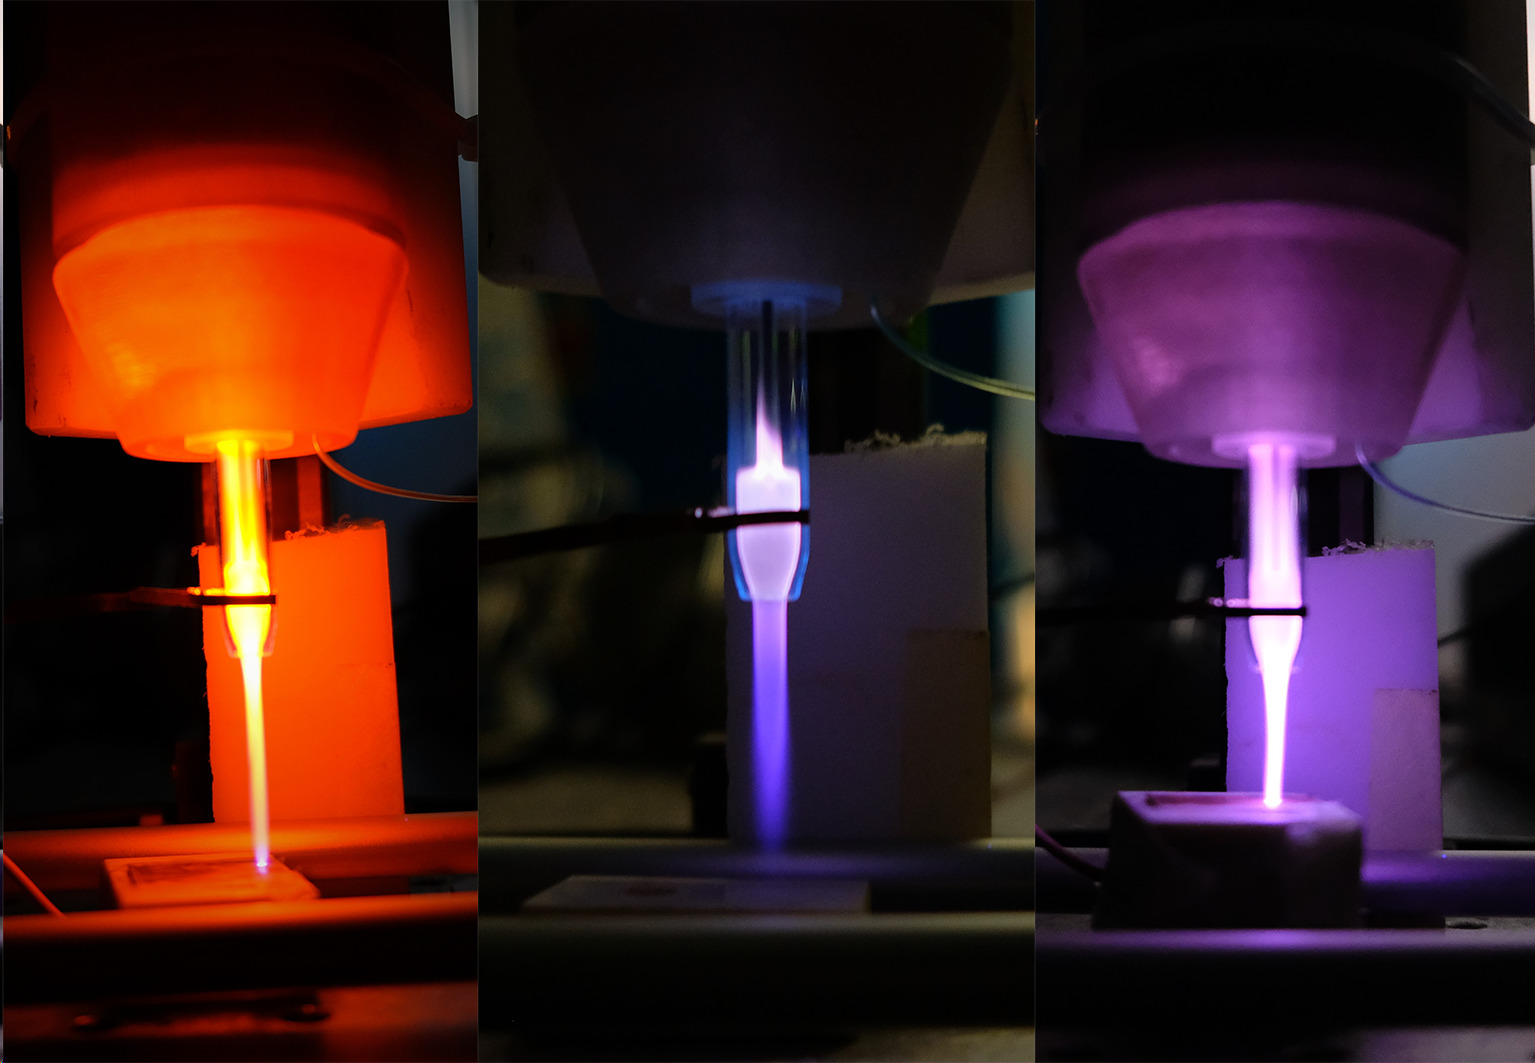
\includegraphics[width = 0.6\textwidth]{Images/Shape/plasmapic.png}
 \caption{Plasma plume pictures with different gasses used to start the discharge: neon on the left, argon in center and helium on the right. The source points to a conductive target positioned in front of the nozzle, after \SI{22}{\milli\meter} for neon and argon, after \SI{14}{\milli\meter} for helium.}
 \label{fig:pl_picture}
\end{figure}
\begin{figure}
 \centering
 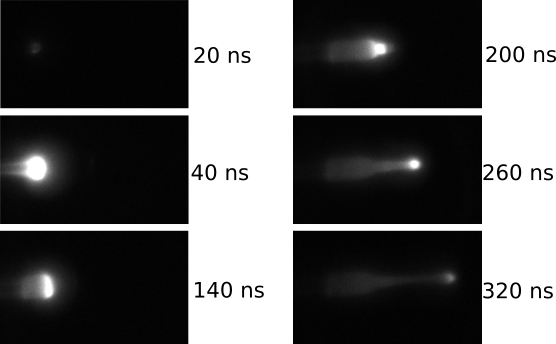
\includegraphics[width=0.8\textwidth]{Images/Shape/frames.png}
 \caption{Example of helium plasma bullet expulsion, as measured with our experimental setup. The single frames are taken with a fast camera with integration time of \SI{15}{\micro\second}.}
 \label{fig:pl_bullet}
\end{figure}

Plasma bullets still needs to be studied in depth, at today are known the basic dynamic of formation and expulsion. Some general features are that:
\begin{itemize}
 \item bullets velocities are $> \SI{10}{\kilo\meter/\second}$;
 \item bullet formation, it's velocity and it's travel distance depend on applied voltage on the electrode.
\end{itemize}

The scope of this experiment is to observe plasma bullets produced by our source, their shape and their velocity and how they change with different discharge conditions.

Given their typical velocities and the temperature of the plasma, bullet propagation is tought to be related to a travelling ionization front. This propagation can be studied with simplified simulation of DBD discharges, where it's reproduced the behaviour of plasma bullets (\cite{doi:10.1063/1.4963115}, \cite{Breden_2012}) or the interaction between plasma and a target (\cite{doi:10.1063/1.4923345}). Possible explanation for bullet propagation are analyzed at the end of this chapter, with estimation of electron temperature and mobility that give better insight on the phenomenology.
%We present a simple 1D model that can reproduce the propagation of this ionization front.

\section{Experimental setup}
To visually observe dynamics of plasma formation and propagation with enough resolution, it is needed an acquisition setup with a fast camera that has short integration time, below \SI{20}{\nano\second}, and an image intensifier that allows to visualize light emitted in such a short time interval.

To guarantee synchrony between plasma discharge and frame acquisition it is necessary to consider instruments and plasma source specific delays and give appropriate triggers.

Experimental setup is shown in photo \ref{fig:fotosetup} and a scheme is presented in \ref{fig:schemashape}. In the scheme there are the voltage signal lines that trigger the discharge and the acquisition, the optical acquisition apparatus pointed at source exit and the measurements acquisition instruments that are a computer and an oscilloscope. 
\begin{figure}
 \centering
 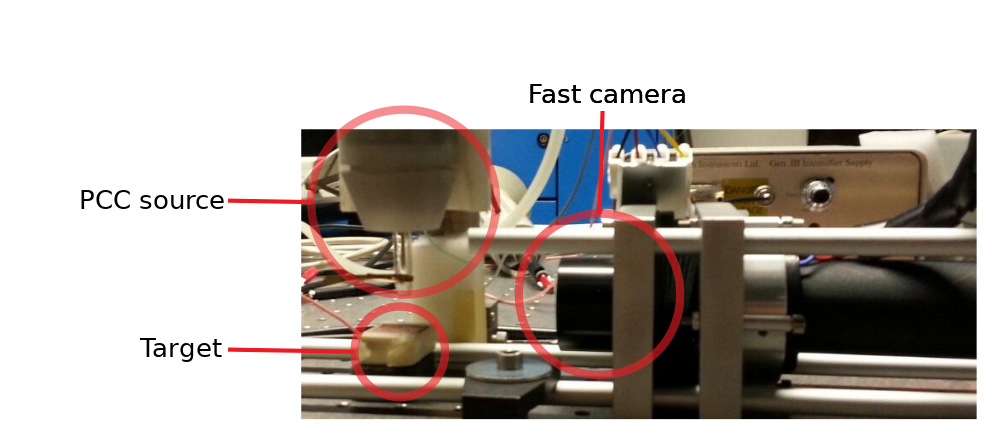
\includegraphics[width=0.8\textwidth]{Images/Shape/app_pic.png}
 \caption{Picture of the experimental setup. The source PCC is mounted vertically and points to a removable target that can be positioned at different heights. Plasma is observed with a fast camera from the side.}
 \label{fig:fotosetup}
\end{figure}
\begin{figure}
 \centering
 
\includegraphics[width=0.5\textwidth]{Images/Shape/acq_ottica.png}
 \caption{Experimental setup scheme. Function generator 1, function generator 2 and delay generator send trigger signal to camera (CCD), to source and to image intensifier (MCP), full lines in the scheme. Camera sends measured frames to a computer (PC). From source, source's target, function generator 2 and delay are taken signals read on the oscilloscope, pointed lines in the scheme.}
 \label{fig:schemashape}
\end{figure}

\subsection{Source and optical setup}
Optical apparatus is composed by a lens %specific
 coupled with a Micro Channel Plate image intensifier (MCP). An MCP works as in figure \ref{fig:MCP}: for every photon received it emits many photons with little angular deviation.
\begin{figure}
 \centering
 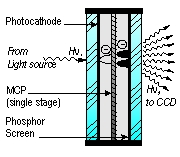
\includegraphics[width=0.4\textwidth]{Images/Shape/MCPsingle-stage.jpg}
 \caption{Micro Channel Plate image intensifier functioning.}
 \label{fig:MCP}
\end{figure}

Those photons are received by an high-speed camera \emph{Point Grey Flea} (\cite{flea}) equipped with a CCD of $\num{1024} \times \num{768}$ square pixels $\SI{4.75}{\micro\meter}$ wide. Every frame is sent to the pc where FLIR software elaborates and saves them in pgm format (\cite{pgm}).

\subsection{Source, power lines and electric signals}
The source utilized is the latest prototype, \textbf{B} in chapter \ref{ch:electric}. It has a voltage pulse peak value between $\num{3}$ and \SI{10}{\kilo\volt}, regulated by the lenght of the trigger signal $\Delta t$ (see chapter \ref{ch:electric}). To synchronyze measures and discharge the trigger signal a generator function gives the trigger signal (generator $2$ in the scheme) instead of the usual controller module of the source.

The source is positioned vertically at a distance of \SI{42.0(1)}{\milli\meter} from optical bench, with the glass nozzle that allows to observe plasma formation inside it (external diameter \SI{8.0(1)}{\milli\meter}, internal diameter \SI{6.0(1)}{\milli\meter}). The distance from the end of the electrode and nozzle exit is \SI{12}{\milli\meter}. At the exit the nozzle shrinks for \SI{3.0(1)}{\milli\meter}, until a diameter of \SI{5.0(1)}{\milli\meter}

Under the source is possible to position targets. Two different targets are used at different heights: a conductive target and an insulating target. The first one is a copper square sheet of dimensions $\SI{10}{\milli\meter} \times \SI{10}{\milli\meter} \times \SI{1}{\milli\meter}$ (used for current measures in chapter \ref{ch:electric}), the second one is a plastic material.

CCD camera is powered by a common voltage supply, while image intensifier MCP is powered by an high voltage supply. A delay generator trigger both instruments, with different delay times (see next section).

The oscilloscope \emph{Yokogawa DL9040}, utilized in chapter \ref{ch:electric}, reads on different channels the trigger signal given to source head, the trigger signal given to MPC, the voltage electrode with high-voltage probe \emph{Tektronix P6015A} and the current intensity when it's used the conductive target. Measurements of current intensity are done by a voltage probe with attenuation $\times \num{10}$ that measures the voltage drop on a resistance of $\SI{1}{\mega\ohm}$ connected to the conductive target.

\subsection{Trigger synchronization}
Experiment's objective is to observe plasma formation and propagation in synchronization with the measurement of voltage on the electrode, so it's necessary to know precisely discharge and measure times.

The trigger lines is composed with:
\begin{itemize}
 \item function generator \emph{Or-x 310}, $1$ in figure, that sends a square pulse with set amplitude and width, with pulse repetition rate $f$;
 \item function generator \emph{Lecroy 9210}, $2$ in figure, that sends a square wave with repetition rate given by the trigger, with constant amplitude and variable width $\Delta t$;
 \item delay time generator \emph{Stanford DG535}, that sends a square wave with constant amplitude and repetition rate given by the voltage input. Start time of this signal is given by input starting time plus settable delays (4 different channels).
\end{itemize}

Every measuring instrument has it's own time delay between trigger signal and effective measure. The higher delay is the arming time for fast camera, in the order of \si{\milli\second}, the shortest one is the integration time for acquisition system, that starts from the activation of the image intensifier and span $\SI{15}{\nano\second}$.

A time line is shown in figure \ref{fig:times}, an example of signals taken with the oscilloscope is in figure \ref{fig:times_signals}. There are three relevant times defined by function and delay generators:
\begin{enumerate}
 \item $t_{0}$ is the starting time for the square pulse given by \emph{Function generator 1}, with an amplitude of $\SI{5}{\volt}$ and repetition rate $f$. The pulse is the external trigger for \emph{Function generator 2} and the voltage input of \emph{Delay generator}. The square wave that triggers the voltage pulse on the source starts at $t_{0}$ from \emph{Function generator 2}; it has a time width of $\Delta t$ that defins voltage amplitude (see chapter \ref{ch:electric}) and repetition rate $f$. The trigger signal that arms the camera starts at $t_{0}$ from \emph{Delay generator}.
 \item $t_{\text{DIS}}$ is the effective discharge starting time, when the voltage peak starts. From trigger signal end to voltage peak start there is a time delay given mainly by the response time of the photodiode on source head. Measuring the signals as in figure \ref{fig:times_signals}, it's possible to estimate this delay as $\SI{987.7(567)}{\nano\second}$, constant for every $f$ and $\Delta t$. The discharge happens after $t_{\text{DIS}}$, measurement times must be inside the grey zone in the scheme.
 \item $t_{\text{MIS}}$ is the measurement time, when MCP is triggered on. \emph{Delay generator} gives the delay between $t_{0}$ and $t_{\text{MIS}}$, called $t_{D}$, with possible steps of \SI{1}{\pico\second}. Changing $t_{D}$ it's possible to see plasma dynamics at different times that corresponds to different electrode voltage values, as in figure \ref{fig:times_signals}.
\end{enumerate}
\begin{figure}
 \centering
 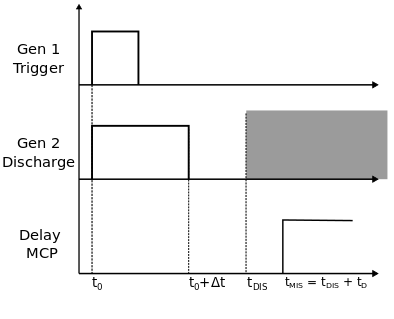
\includegraphics[width=0.6\textwidth]{Images/Shape/times.png}
 \caption{Time signal synchronization scheme: $t_{0}$ is the starting trigger time, $\Delta t$ is the opening time for plasma source (see chapter \ref{ch:electric}), $t_{\text{DIS}}$ is the starting time for the discharge and $t_{\text{MIS}}$ the starting time for the MCP i.e. the measure time}.
 \label{fig:times}
\end{figure}
\begin{figure}
 \centering
 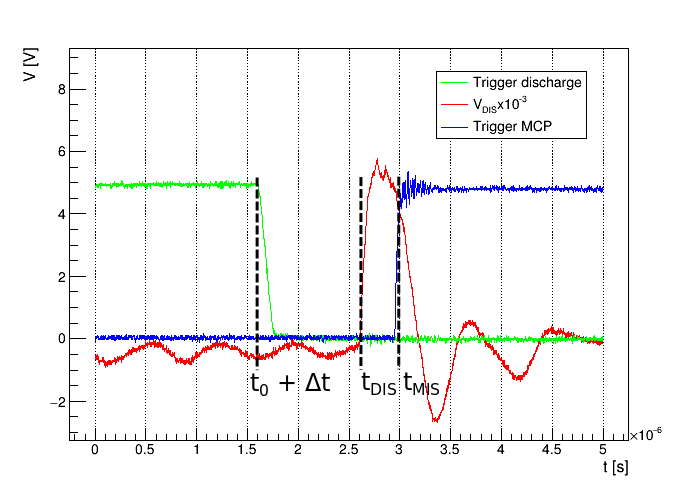
\includegraphics[width=0.6\textwidth]{Images/Shape/times_osc_2.png}
 \caption{Example of oscilloscope measure. In green the discharge trigger, in red the electrode voltage output and in blue the MCP trigger. The dashed lines indicate times described in \ref{fig:times}.}
 \label{fig:times_signals}
\end{figure}


Integration time for a single frame is \SI{15}{\nano\second}, so the time step between two measures has to be larger then it. Time steps chosen are \SI{20}{\nano\second} for high resolution mesurements, \SI{50}{\nano\second} for standard measurements.

It's important to point out that pulse repetition rates are $f \ge \SI{1}{\kilo\hertz}$ corresponding to a time interval between two pulses lower then \SI{1}{\milli\second}; while the measure interval time between the acquisition of two frames is larger then \SI{50}{\milli\second} beacause of the camera. It is not possible to see two consecutive times for the same discharge, the frames are always measures of different discharges.

Eaxh pixel on the CCD has a minimum and maximum intensity value, is possible to mantain the measure on the wanted level changing the settings on camera acquisition software.
One of the parameters is the \emph{Shutter time}, the opening time of the camera shutter. If the emission intensity is too low we can set the shutter time larger then the time between two acquisition, to acquire a frame that is the sum of two discharge.
Another parameter is the \emph{Gain} value, that amplifies or reduces the output.
For each used gas we select an appropriate \emph{Gain} value and an appropriate \emph{Shutter time}.

\subsection{Different setups}
Many parameters have an effect on plasma formation: voltage pulse repetition rate, voltage rise time, voltage peak value, gas type, gas flow, presence of a target and its features (see \cite{Mericam_Bourdet_2009}, \cite{Jarrige_2010}).
This study presents different setups with three different gasses, as shown in table \ref{tab:setups}.
There is a lower limit value for pulse repetition rate, different for each gas, under which there is no discharge. The electric behavior of the source is the same for values higher than this threshold (see chapter \ref{ch:electric}). For each gas is chosen a repetition rate value that allows the discharge to start.

Gasses with different composition will have different ionization reactions and will produce different reactive species, with different masses and ionization energies. With this study is possible to observe how peak voltage value, gas type and gas flow determine plasma bullet formation and affect its expulsion velocity.

A conductive target near plasma exit at ground potential will modify the electric field produced by the electrode. With this study is possible to observe how the target affects bullet expulsion and propagation. Furthermore the bullet can hit the target, introducing into reactions balance also the electrons on the target.

When argon is the neutral gas used to start the discharge a grounded conductive ring can be placed around the nozzle after the electrode, to help the start of the discharge.
\begin{table}
 \centering
 \begin{tabular}{cccccccc}
  \toprule
  Gas   &Setup  &$\Delta t$ [\si{\micro\second}] &Target &Target position [\si{\milli\meter}] &Flow rate [\si{\liter/\minute}]  &Other  &$\Delta t_D$ [\si{\nano\second}]\\
  \midrule
  \multirow{7}*{\ce{He}}    &A  &\num{3}, \num{3.5}, \num{4} &-  &-  &\num{2} &-  &\num{20}\\
                            &B  &\num{3.5} &-  &-  &\num{1}  &-  &\num{20}\\
                            &C  &\num{3.5} &-  &-  &\num{3}  &-  &\num{20}\\
                            &D  &\num{3.5} &-  &-  &\num{4}  &-  &\num{20}\\
                            &E  &\num{3}, \num{3.5}, \num{4} &Insulator  &\num{24}  &\num{2} &-  &\num{20}\\
                            &F  &\num{3}, \num{3.5}, \num{4} &Conductor  &\num{32}  &\num{2} &-  &\num{20}\\
                            &G  &\num{3}, \num{3.5}, \num{4} &Conductor  &\num{24}  &\num{2} &-  &\num{20}\\
  \midrule
  \multirow{4}*{\ce{Ne}}    &A  &\num{2}, \num{2.5}, \num{3} &Insulator  &\num{24}  &\num{2} &-  &\num{50}\\
                            &B  &\num{2}, \num{2.5}, \num{3} &Conductor  &\num{32}  &\num{2} &-  &\num{50}\\
                            &C  &\num{2}, \num{2.5}, \num{3} &Conductor  &\num{24}  &\num{2} &-  &\num{50}\\
                            &D  &\num{2}, \num{2.5}, \num{3} &-  &-  &\num{2} &-  &\num{50}\\
  \midrule
  \multirow{6}*{\ce{Ar}}    &A  &\num{3.5} &-  &-  &\num{2} &Grounded ring  &\num{50}\\
                            &B  &\num{3.5} &-  &-  &\num{2} &-  &\num{50}\\
                            &C  &\num{3.5} &Conductor  &\num{20}  &\num{2} &Grounded ring  &\num{50}\\
                            &D  &\num{3.5} &Conductor  &\num{20}  &\num{2} &-  &\num{50}\\
  \bottomrule
 \end{tabular}
 \caption{Description of measure setups. In first column there is the gas; second column is the setup name; third column is voltage pulse time width; four and fifth columns are target information, if it's used a target; sixth column is gas flow; seventh column are other informations, e.g. if it's positioned a grounded ring around the nozzle; eight column is the time step between acquisitions.}
 \label{tab:setups}
\end{table}

\begin{comment}
\begin{table}
 \centering
 \begin{tabular}{cccccccc}
  \toprule
  Gas   &Setup  &$\Delta t$ [\si{\micro\second}] &Target &Target position    &Flow rate  &Other  &$\Delta t_D$ [\si{\nano\second}]\\
  \midrule
  \multirow{8}*{\ce{He}}    &A  &$\num{30}, \num{35}, \num{40}$ &Conductor  &\SI{24}{\milli\meter}  &\SI{2}{\liter/\minute} &-  &\SI{50}{\nano\second}\\
                            &B  &$\num{30}, \num{35}, \num{40}$ &Conductor  &\SI{32}{\milli\meter}  &\SI{2}{\liter/\minute} &-  &\SI{20}{\nano\second}\\
                            &C  &$\num{30}, \num{35}, \num{40}$ &Insulator  &\SI{24}{\milli\meter}  &\SI{2}{\liter/\minute} &-  &\SI{20}{\nano\second}\\
                            &D  &$\num{30}, \num{35}, \num{40}$ &-  &-  &\SI{2}{\liter/\minute} &-  &\SI{20}{\nano\second}\\
                            &E  &$\num{35}$ &-  &-  &\SI{2}{\liter/\minute} &Ground ring  &\SI{20}{\nano\second}\\
                            &F  &$\num{35}$ &-  &-  &\SI{1}{\liter/\minute} &-  &\SI{20}{\nano\second}\\
                            &G  &$\num{35}$ &-  &-  &\SI{3}{\liter/\minute} &-  &\SI{20}{\nano\second}\\
                            &H  &$\num{35}$ &-  &-  &\SI{4}{\liter/\minute} &-  &\SI{20}{\nano\second}\\
  \midrule
  \multirow{5}*{\ce{Ne}}    &A  &$\num{20}, \num{25}, \num{30}$ &Conductor  &\SI{24}{\milli\meter}  &\SI{2}{\liter/\minute} &-  &\SI{50}{\nano\second}\\
                            &B  &$\num{20}, \num{25}, \num{30}$ &Conductor  &\SI{32}{\milli\meter}  &\SI{2}{\liter/\minute} &-  &\SI{50}{\nano\second}\\
                            &C  &$\num{20}, \num{25}, \num{30}$ &Insulator  &\SI{24}{\milli\meter}  &\SI{2}{\liter/\minute} &-  &\SI{50}{\nano\second}\\
                            &D  &$\num{20}, \num{25}, \num{30}$ &-  &-  &\SI{2}{\liter/\minute} &-  &\SI{50}{\nano\second}\\
                            &E  &$\num{30}$ &-  &-  &\SI{2}{\liter/\minute} &Ground ring  &\SI{50}{\nano\second}\\
  \midrule
  \multirow{6}*{\ce{Ar}}    &A  &$\num{35}$ &-  &-  &\SI{2}{\liter/\minute} &Ground ring  &\SI{50}{\nano\second}\\
                            &B  &$\num{35}$ &-  &\SI{32}{\milli\meter}  &\SI{2}{\liter/\minute} &-  &\SI{20}{\nano\second}\\
                            &C  &$\num{35}$ &-  &-  &\SI{2}{\liter/\minute} &Floating ring  &\SI{50}{\nano\second}\\
                            &D  &$\num{35}$ &Conductor  &\SI{20}{\milli\meter}  &\SI{2}{\liter/\minute} &Ground ring  &\SI{50}{\nano\second}\\
                            &E  &$\num{35}$ &Conductor  &\SI{20}{\milli\meter}  &\SI{2}{\liter/\minute} &-  &\SI{50}{\nano\second}\\
                            &F  &$\num{35}$ &-  &-  &\SI{2}{\liter/\minute} &-  &\SI{50}{\nano\second}\\
                            &G  &$\num{35}$ &Conductor  &\SI{32}{\milli\meter}  &\SI{2}{\liter/\minute} &-  &\SI{50}{\nano\second}\\
  \bottomrule
 \end{tabular}
 \caption{Description of measure setups. In first column there is the gas; second column is the setup name; third column is voltage pulse time width, expressed as percentage of a square trigger \SI{10}{\micro\second} long; four and fifth columns are target information, where it's used a target; sixth column is used gas flow; seventh column are other informations, i.e. if it's used the conductor ring explained before; eight column is the time step between two different frames.}
 \label{tab:setups}
\end{table}
\end{comment}

\subsection{Frame analysis and calibration}
Once a measure setup is chosen, the first acquisition is set around the start of the discharge. On the oscilloscope is saved the signal waveform for every channel (setup as explained before), on the computer $5$ frames for every $t_D$ are saved. Measures are taken with steps of $\Delta t_D$ until it is not possible to observe plasma anymore.

Measure time from the start of the discharge can be evaluated from waveforms on the oscilloscope.

Frame analysis is done converting the pgm files in 2-dimensional histograms, with \emph{TH2} class written in \emph{ROOT} libraries (see \cite{ROOT:TH2}).
%We are interested in plasma bullet formation and it's expulsion, but also in other fenomenological behaviour that is observed during measures.

From the five frames taken it is evaluated the average value for each pixel. From the resulting frame the plasma bullet is isolated as the collection of pixels with maximum intensity in the frame. The estimation of the bullet position is given by the coordinates of its luminosity barycenter on the plane seen by camera, called x-y in the analysis.
Once established the center, the points were luminosity goes under a certain percentage of the maximum define its contour. Bullet dimensions along x and y axis are evaluated from the contour, while average luminosity is given by pixel values inside the contour.
With barycenter coordinates it's possible to compute bullet velocity using a finite difference formula \cite{Bhadauria}.


Frame dimensions are found through a calibration with a known target: at plasma exit is positioned a plate with $4$ holes, diameter of \SI{1.0(1)}{\milli\meter} at the vertices of a square with an edge lenght of \SI{10.0(1)}{\milli\meter}, and illuminated from behind with a torch.
For the frame of this setup it's possible to extrapolate the pixel distance that corresponds to \SI{10}{\milli\meter} for every square edge, average them, and calculate pixel's width in frames, resulting a value of $d_{pix} = \SI{0.172(2)}{\milli\meter}$.


\section{Helium flow}
Helium it's an element with standard atomic weight of $\num{4.002}$, 1st ionization energy of \SI{24.587}{\electronvolt} and 2nd ionization energy of \SI{54.418}{\electronvolt}.
It is easy to produce helium plasma, when ionized it emits radiation with principal wavelengths in violet and orange ($\lambda = \num{388.86}$ and \SI{587.56}{\nano\meter}).

In this work helium plasma is produced with pulse repetition rate $f = \SI{5}{\kilo\hertz}$ and different voltage peak values, as explained in table \ref{tab:setups}.
Delays are setted to take a single frame during every acquisition, for every measure are acquired $5$ frames.

\subsection{Plasma bullet description}
A description of bullet propagation can be given with setup A, for $\Delta t = \SI{3.5}{\micro\second}$, i.e. absence of a target and gas flow of \SI{2}{\liter/\minute}.

It's possible to divide the phenomenon in four phases, as presented in figure \ref{fig:bullet_es}: bullet formation, bullet displacement inside the nozzle, bullet expulsion and bullet propagation outside the nozzle, in air. %It's important to remember that time values goes from the start of the voltage peak, extrapolated from oscilloscope measures.
When the voltage goes over a definite value, a rapid increase in luminosity is observed around the electrode. From there, in a time of $\sim \SI{50}{\nano\second}$ the plasma modifies it'shape and becames the bullet: a zone with high luminosity confined in space. The bullet then moves in the exit direction and it's expelled always with a well defined front. The round shaped bullet propagation can be seen in air until it reaches a maximum travel distance and then luminosity decreases rapidly. In these measurements conditions plasma forms again in correspondence of the negative tension peak, but it is a rapid process without propagation.
\begin{figure}
 \centering
 \subfloat[\SI{140.93}{\nano\second}]{
    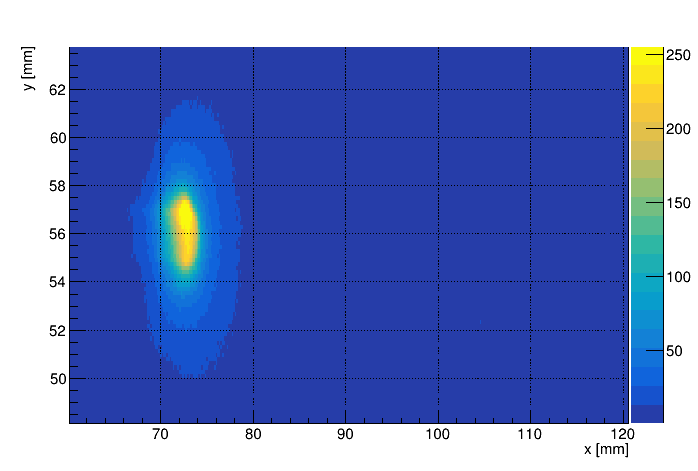
\includegraphics[width=0.48\textwidth]{Images/Shape/elio_d035_es1.png}
 }
 \hfill
 \subfloat[\SI{240.93}{\nano\second}]{
    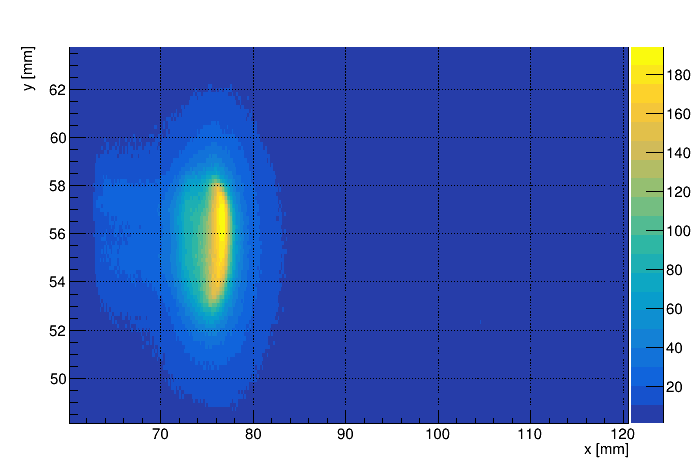
\includegraphics[width=0.48\textwidth]{Images/Shape/elio_d035_es2.png}
 }
 
 \subfloat[\SI{400.93}{\nano\second}]{
    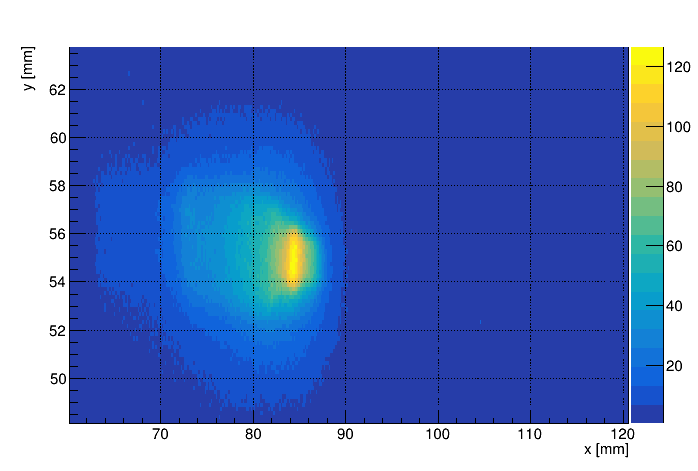
\includegraphics[width=0.48\textwidth]{Images/Shape/elio_d035_es3.png}
 }
 \hfill
 \subfloat[\SI{460.93}{\nano\second}]{
    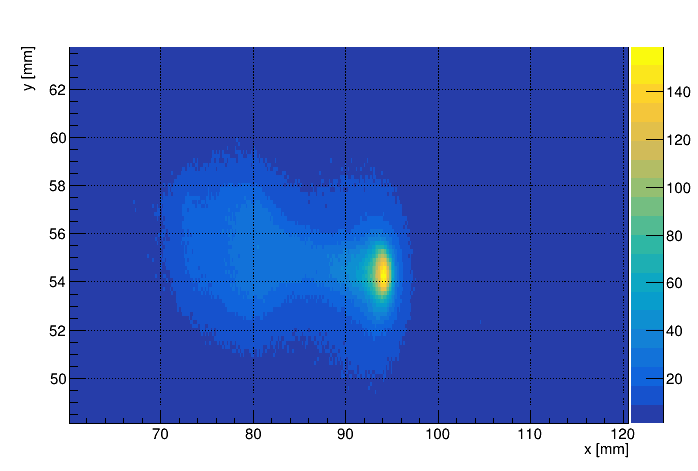
\includegraphics[width=0.48\textwidth]{Images/Shape/elio_d035_es4.png}
 }
 \caption{Four phases of plasma dynamics: bullet formation (a), bullet displacement inside the nozzle (b), bullet expulsion (c) and bullet propagation outside the nozzle (d). Time intervals are calculated from the start of the voltage peak.}
 \label{fig:bullet_es}
\end{figure}


\paragraph{Electrode voltage and bullet intensity}
The time interval where there is the bullet can be defined as where it is possible to see a definite zone with mean luminosity higher then the background. The starting time is given by voltage reaching a certain value, and the bullet expires when it's luminosity decreases.

The average intensity value inside the bullet and the voltage measurement in the intersted time interval are presented in figure \ref{fig:elio_d035_I}. Plasma formation is observed around \SI{120.93}{\nano\second} after peak start, at a tension value of \SI{5710.00(28550)}{\volt}. %while maximum peak value is \SI{6588.80(32944)}{\volt} at time \SI{260.93}{\nano\second}.
Luminosity is higher during plasma formation around the electrode and it decrease very little during all the propagation, even after the expulsion in air (pointed line on the graph). After a time of \SI{440}{\nano\second} the bullet luminosity decreases rapidly and it disperses in the air.
\begin{figure}
 \centering
 \subfloat[Zoom on voltage waveform.]{
    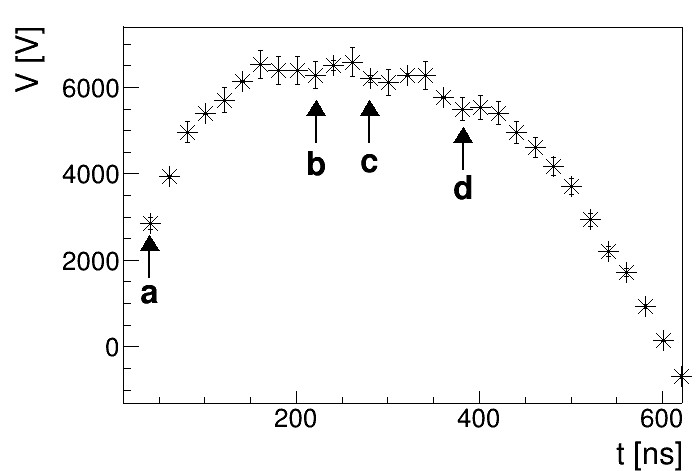
\includegraphics[width=0.48\textwidth]{Images/Shape/elio_d035_V.png}
 }
 \hfill
 \subfloat[Mean intensity of plasma bullet.]{
    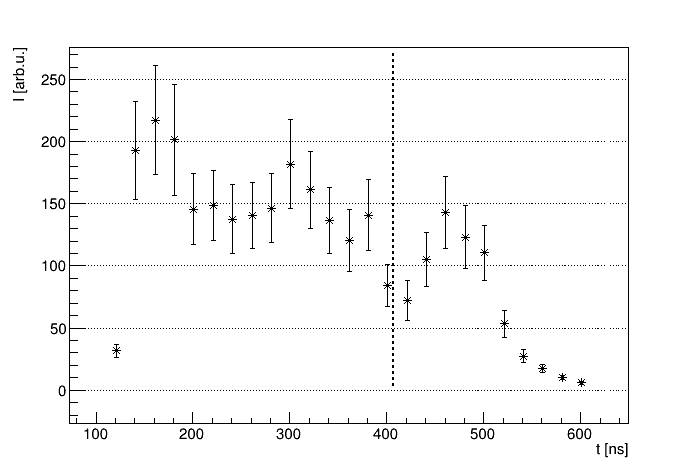
\includegraphics[width=0.48\textwidth]{Images/Shape/elio_d035_Im.png}
 }
 \caption{Voltage waveform and intensity of the bullet versus time, measurements setup A with voltage peak of \SI{6.6}{\kilo\volt}. Time zero is the start of the voltage peak, ending time is taken as the time where intensity reaches background value. The dashed line for intensity indicates when the bullet reaches the end of the nozzle.}
 \label{fig:elio_d035_I}
\end{figure}

\paragraph{Barycenter coordinates and direction}
The motion of the bullet on observing plane can be extrapolated from its barycenter coordinates.

In figure \ref{fig:elio_d035_bary} there are the two coordinates for different times.
Coordinate x, along the axis of the source is more relevant to observe bullet expulsion. Plasma forms around position $\SI{73}{\milli\meter}$ and the nozzle ends at $\SI{85}{\milli\meter}$, compatible with the distance described before. Plasma bullet moves in the nozzle with a certain velocity, until it reaches the exit and propagates in the air more rapidly. In air the bullet travels until it reaches a maximum x, covering a distance of \SI{26.08(2)}{\milli\meter} from the electrode. The bullet stops before its luminosity reaches the minimum value.

Coordinate y it's relevant to show bullet direction. From figure it is possible to see that  it moves in a space interval of \SI{2}{\milli\meter}. The bullet forms over the electrode, then it enlarges to cover all the nozzle diameter and lowers it's barycenter with a constant slope, even after the expulsion. Once the bullet starts to decrease in luminosity, it stops its motion also on the y direction.
\begin{figure}
 \centering
 \subfloat[]{
    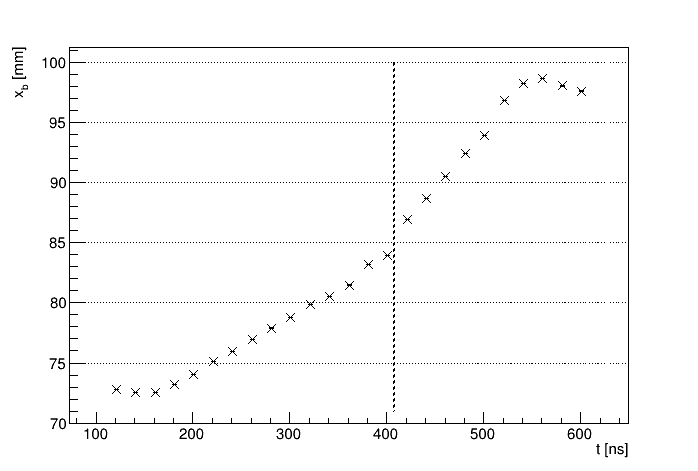
\includegraphics[width=0.48\textwidth]{Images/Shape/elio_d035_xb.png}
 }
 \hfill
 \subfloat[]{
    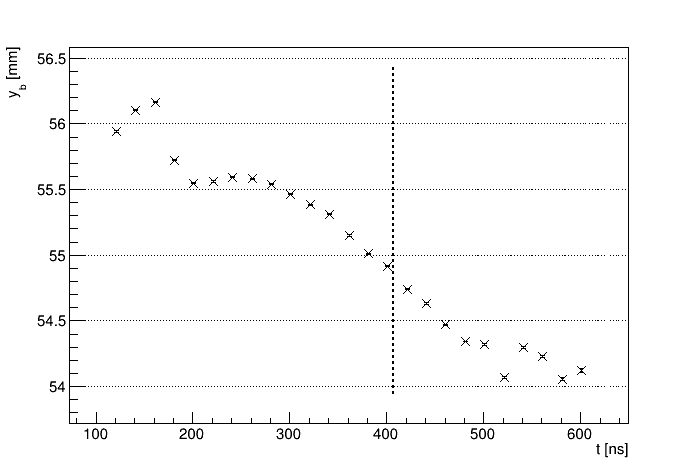
\includegraphics[width=0.48\textwidth]{Images/Shape/elio_d035_yb.png}
 }
 \caption{Barycenter coordinates of the bullet for measurements setup A with voltage peak of \SI{6.6}{\kilo\volt}. Pointed lines indicate the end of the nozzle.}
 \label{fig:elio_d035_I}
\end{figure}

Baricenter motion in the y direction it's explainable by a tilt in the source, that is not perfectly perpendicular to the optical bench. In figure \ref{fig:elio_d035_diry} there is the countour of the bullet in the y direction in function of the x brycenter coordinate, is possible to see that the figure is inclined. Inside the nozzle y maximum is the value that defines the contour of the nozzle, the angle of inclination is given by a linear fit as in figure and it is \SI{3.39(10)}{\degree}. Outside the nozzle the barycenter direction is inclined at an angle of \SI{3.71(4)}{\degree}. The values are almost compatible with each other, so it seems that tilting the source it is possible to direct the bullet even after its propagation in air.
\begin{figure}
 \centering
 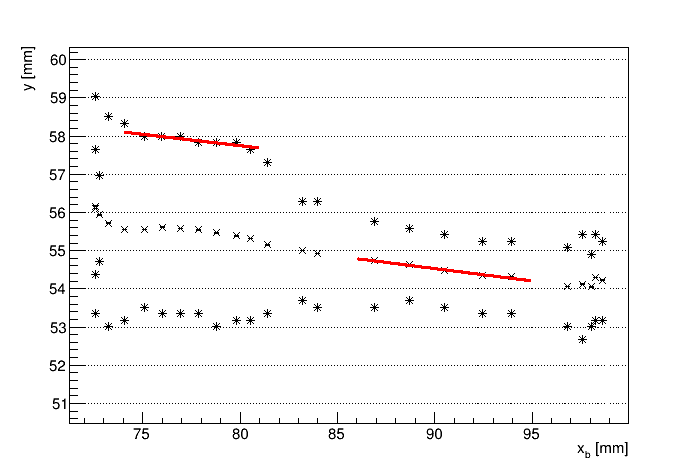
\includegraphics[width=0.6\textwidth]{Images/Shape/elio_d035_incl.png}
 \caption{Countour of the bullet in y direction as a function of barycenter coordinate x, for measurements setup A with voltage peak of \SI{6.6}{\kilo\volt}. For each x value is possible to see y maximum, y minimum and y barycenter of the bullet. There are two linear fits to compare the inclination of the source (first linear fit of y maximum inside the nozzle) with the inclination of bullet propagation direction in air (second linear fit of y barycenter).}
\end{figure}


\paragraph{Bullet dimensions}
Once the contour of the bullet is defined, it is simple to evaluate its dimensions along x and y directions, in figure \ref{fig:elio_d035_dim} are presented the results for each time.
.
In the x direction, the bullet presents constant diameter until it approaches nozzle exit, where it enlarges to reach the exit. In air the bullet mantaines its dimension, with lower values then inside the nozzle, but compatible within the error. When it stops the measure loses significance as the bullet loses luminosity and it is not distinguishable from the background.
In y direction there is a constant value of \SI{4.65(20)}{\milli\meter} during propagation in the nozzle, as expected because the bullet covers all the nozzle area. Once the nozzle shrinks, the bullet diminish it's diameter and maintains a constant value of \SI{2.07(20)}{\milli\meter} during all the propagation in air.
\begin{figure}
 \centering
 \subfloat[]{
    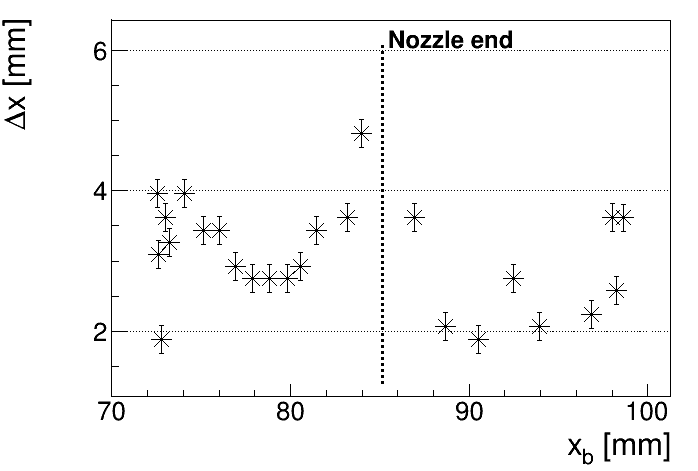
\includegraphics[width=0.48\textwidth]{Images/Shape/elio_d035_dx.png}
 }
 \hfill
 \subfloat[]{
    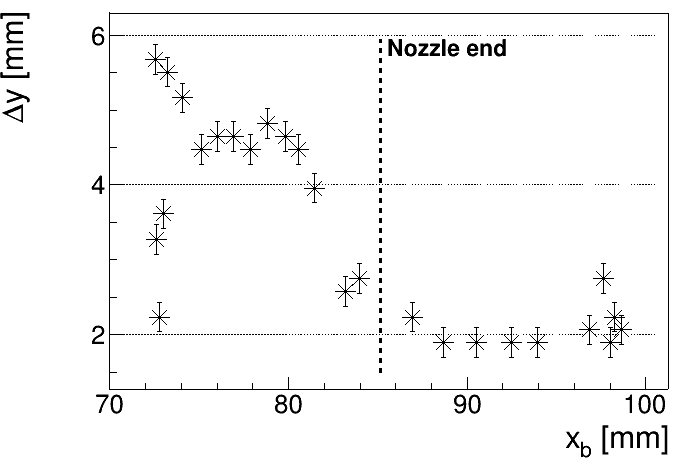
\includegraphics[width=0.48\textwidth]{Images/Shape/elio_d035_dy.png}
 }
 \caption{Dimensions of the bullet for measurements setup A with voltage peak of \SI{6.6}{\kilo\volt}. Pointed lines indicate the end of the nozzle.}
 \label{fig:elio_d035_I}
\end{figure}


\paragraph{Bullet velocity}
From barycenter graphs it is possible to estimate the bullet velocity at different times.
With a linear fit of the x barycenter inside the nozzle, as shown in figure \ref{fig:elio_d035_vx}, bullet velocity is found to be $v_{N} = \SI{46.48(20)}{\kilo\meter/\second}$. Once it exits the nozzle the speed goes up, until a value of $v_{A} = \SI{95.16(60)}{\kilo\meter/\second}$.

Velocity for each time can be calculated with a 3 point finite difference formula (that excludes the first and the last point), finding the values shown in figure \ref{fig:elio_d035_vx}. The average velocity value inside the nozzle and in air is compatible with the result from the linear fit: $v_{N} = \SI{48.23(103)}{\kilo\meter/\second}$ and $v_{A} = \SI{95.16(182)}{\kilo\meter/\second}$.
\begin{figure}
 \centering
 \subfloat[Fit of x barycenter.]{
    \includegraphics[width=0.48\textwidth]{Images/Shape/elio_d035_xb_fitv.png}
 }
 \hfill
 \subfloat[Velocities in x direction.]{
    \includegraphics[width=0.48\textwidth]{Images/Shape/elio_d035_vx_fitv.png}
 }
 \caption{Velocity of the bullet in x direction for measurements setup A with voltage peak of \SI{6.6}{\kilo\volt}. In (a) linear fit of barycenter position as function of time inside the nozzle and in air; in (b) velocities evaluated for each time with a three point difference formula, where dashed lines indicate average values inside the nozzle and in air.}
 \label{fig:elio_d035_vx}
\end{figure}

It's interesting to point out that those velocities are much higher then the average velocity of the neutral gas: for a flow of \SI{2}{\liter/\minute} it is of \SI{12}{\meter\second}.


\subsection{Voltage influence}
An increase in trigger width $\Delta t$ correspond to an increase in voltage peak values (see chapter \ref{ch:electric}) and an increase in electric field intensity. The voltage peak value could change bullet formation and propagation. The results of the analysis for setup A with different voltage values are in figure \ref{fig:elio_d} and table \ref{tab:elio_d}.

The discharge starts always in the same voltage interval, around \SI{5.7}{\kilo\volt}. At an higher voltage corresponds an higher luminosity, but the time interval where luminosity decreases is always around \SI{100}{\nano\second} once it exits the nozzle (figure \ref{fig:elio_d} (a)).

The plot for the barycenter coordinates (figure \ref{fig:elio_d} (b) - (c)) shows that higher voltage corresponds to further distances reached by the bullet ($x_{\text{dist}}$ and $y_{\text{dist}}$ in table). For the lower voltage peak the bullet doesn't even propagate in air, as it stops right after nozzle exit.

Dimensions of the bullet (figure \ref{fig:elio_d} (d) - (e)) are not influenced by voltage value, they have the exact same behaviour for every measurements set. A single notable difference it's in the y diameter inside the nozzle, where for higher voltage there are slightly larger values. However inside the nozzle there are refraction effects due to the glass, the increase is compatible with the variation in dimensions that could be given by higher luminosity.

Velocity values (figure \ref{fig:elio_d} (f)) show how the bullet behaviour is costant during the propagation inside the nozzle and becames more erratic once it exits.
As mentioned before, for the lowest voltage value the bullet stops right after it exits the nozzle, in this configuration it's not possible to find a propagation velocity in air. For other sets velocity has the same profile, with a proportionality between peak voltage value and velocity value: increasing voltage velocity goes from $v_{A} = \SI{92.93(6)}{\kilo\meter/\second}$ to $v_{A} = \SI{149.47(9)}{\kilo\meter/\second}$.
\begin{figure}
 \centering
 \subfloat[Mean luminosity.]{
    \includegraphics[width=0.48\textwidth]{Images/Shape/elio_d_Im.png}
 }
 \hfill
 \subfloat[x barycenter.]{
    \includegraphics[width=0.48\textwidth]{Images/Shape/elio_d_xb.png}
 }
 \subfloat[y barycenter.]{
    \includegraphics[width=0.48\textwidth]{Images/Shape/elio_d_yb.png}
 }
 \hfill
 \subfloat[x diameter.]{
    \includegraphics[width=0.48\textwidth]{Images/Shape/elio_d_dx.png}
 }
 \subfloat[y diameter.]{
    \includegraphics[width=0.48\textwidth]{Images/Shape/elio_d_dy.png}
 }
 \hfill
 \subfloat[x velocity.]{
    \includegraphics[width=0.48\textwidth]{Images/Shape/elio_d_vx.png}
 }
 \caption{Results of the analysis for setup A (helium flow of \SI{2}{\liter/\minute} without target), with different peak voltage values.}
 \label{fig:elio_d}
\end{figure}

\begin{comment}
\begin{table}
 \centering
 \begin{tabular}{ccccccc}
 \toprule
 $V_{p}$ [kV]    &$t_{0}$ [ns] &$V_{0}$ [kV]    &$x_{\text{dist}}$ [mm]   &$y_{\text{dist}}$ [mm]   &$v_{N}$ [km/s]   &$v_{A}$ [km/s]\\
 \midrule
 \num{5.66(30)}  &\num{131.5}  &\num{5.55(28)}    &\num{15.99(1)} &\num{1.66(2)}  &\num{37.72(4)} &-\\
 \num{6.59(33)}  &\num{120.9}  &\num{5.71(29)}    &\num{26.08(2)} &\num{1.92(4)}  &\num{46.48(2)} &\num{95.16(6)}\\
 \num{7.22(36)}  &\num{119.5}  &\num{6.01(30)}    &\num{34.55(5)} &\num{2.07(1)}  &\num{59.80(3)} &\num{149.47(9)}\\
 \bottomrule
 \end{tabular}
 \caption{Result of the analysis with different voltage peak values for the pulse. $V_{p}$ is the peak value for the pulse, $t_{0}$ bullet formation time, $V_{0}$ bullet formation tension, $x_{\text{dist}}$ and $y_{\text{dist}}$ are the highest distances reached by the bullet from electrode position, $v_{N}$ is the velocity in x direction reached inside the nozzle, $v_{A}$ is the velocity of propagation in air in x direction.}
 \label{tab:elio_d}
\end{table}
\end{comment}

\begin{table}
 \centering
 \begin{tabular}{cccccc}
 \toprule
 $V_{p}$ [kV]    &$V_{0}$ [kV]    &$x_{\text{dist}}$ [mm]   &$y_{\text{dist}}$ [mm]   &$v_{N}$ [km/s]   &$v_{A}$ [km/s]\\
 \midrule
 \num{5.66(30)}  &\num{5.55(28)}    &\num{15.99(1)} &\num{1.66(2)}  &\num{37.72(4)} &-\\
 \num{6.59(33)}  &\num{5.71(29)}    &\num{26.08(2)} &\num{1.92(4)}  &\num{46.48(2)} &\num{95.16(6)}\\
 \num{7.22(36)}  &\num{6.01(30)}    &\num{34.55(5)} &\num{2.07(1)}  &\num{59.80(3)} &\num{149.47(9)}\\
 \bottomrule
 \end{tabular}
 \caption{Result of the analysis for measurements setup A. $V_{p}$ is the voltage peak value, $V_{0}$ is the voltage value at plasma formation time, $x_{\text{dist}}$ and $y_{\text{dist}}$ are the highest distances reached by the bullet from electrode position, $v_{N}$ is the velocity in x direction reached inside the nozzle, $v_{A}$ is the velocity of propagation in air in x direction.}
 \label{tab:elio_d}
\end{table}


\subsection{Flow influence}
As said before, neutral gas velocity is low if compared to bullet speed, however it could influence the overall dynamic of bullet propagation. Setup A, B, C and D correspond to four different flows with the same peak voltage. In figure \ref{fig:elio_flow} and table \ref{tab:elio_flow} are presented the results of the analysis.

Also for this parameter, the discharge starts always in the same voltage interval, for values higher then \SI{5.7}{\kilo\volt}. For gas flows of $\num{1}$ and \SI{2}{\liter/\minute} bullet luminosity decreases in a time interval around \SI{100}{\nano\second} once it exits the nozzle. For flows $> \SI{2}{\liter/\minute}$ it has luminosity clearly stronger then background for a longer time interval, around \SI{200}{\nano\second} (figure \ref{fig:elio_flow} (a)).

From the barycenter coordinates (figure \ref{fig:elio_flow} (b) - (c)) can be seen that more gas flow is correlated with lower mobility of the bullet: it propagates for shorter distances  when there are higher flows. For maximum flow, even if bullet luminosity is comparable to the other measurements, the bullet travels a short distance from the exit of the nozzle and its barycenter stays in the same position until bullet luminosity reaches background value.

\begin{comment}
Inside the no Width of the bullet increases with increasing and gas flow (figure \ref{fig:elio_d} (d) - (e)) is an inverse proportionality: For stronger flows we have always littler diameters inside the nozzle, in both directions.
\end{comment}

The study of bullet's velocity can give more insight to the phenomenology of bullet propagation, it is shown in figure \ref{elio_flow} (e), with higher detail for values inside the nozzle in figure \ref{elio_flow} (f). Bullet's velocity always decreases moving inside the nozzle, until it reaches a certain distance. The deceleration inside the nozzle is more evident with higher flow, expecially when the flow is higher then \SI{3}{\liter/\minute} (as we can see also in \cite{Jarrige_2010}). The distance at which the bullet speeds up is different for different flows as can be seen in table \ref{tab:elio_Re}.
Once the bullet exits from the nozzle, its velocity decreases more rapidly with higher gas flow.
\begin{figure}
 \centering
 \subfloat[Mean luminosity.]{
    \includegraphics[width=0.48\textwidth]{Images/Shape/elio_035_Im.png}
 }
 
 \subfloat[x barycenter.]{
    \includegraphics[width=0.48\textwidth]{Images/Shape/elio_035_xb.png}
 }
 \hfill
 \subfloat[y barycenter.]{
    \includegraphics[width=0.48\textwidth]{Images/Shape/elio_035_yb.png}
 }
 
 \subfloat[x diameter.]{
    \includegraphics[width=0.48\textwidth]{Images/Shape/elio_035_dx.png}
 }
 \hfill
 \subfloat[y diameter.]{
    \includegraphics[width=0.48\textwidth]{Images/Shape/elio_035_dy.png}
 }
 
 \subfloat[x velocity.]{
    \includegraphics[width=0.48\textwidth]{Images/Shape/elio_035_vx.png}
 }
 \hfill
 \subfloat[x velocity inside the nozzle.]{
    \includegraphics[width=0.48\textwidth]{Images/Shape/vnoz_flux_zoom.png}
 }
 \caption{Results of the analysis for setup A, B, C and D: different gas flow, voltage peak value of \SI{5.7}{\kilo\volt}, without target.}
 \label{fig:elio_flow}
\end{figure}

\begin{table}
 \centering
 \begin{tabular}{cccccc}
 \toprule
 Flow [L/min]    &$V_{0}$ [kV]    &$x_{\text{dist}}$ [mm]   &$y_{\text{dist}}$ [mm]   &$v_{N}$ [km/s]   &$v_{A}$ [km/s]\\
 \midrule
 \num{1}  &\num{5.87(8)}    &\num{30.65(3)} &\num{2.75(1)}  &\num{54.33(10)} &\num{113.97(9)}\\
 \num{2}  &\num{5.71(29)}    &\num{26.08(2)} &\num{1.92(4)}  &\num{46.48(2)} &\num{95.16(6)}\\
 \num{3}  &\num{5.41(27)}    &\num{19.38(1)} &\num{1.84(1)}  &\num{39.88(4)} &\num{80.96(30)}\\
 \num{4}  &\num{5.90(12)}    &\num{22.80(3)} &\num{2.30(1)}  &\num{58.89(14)} &\num{41.94(44)}\\
 \bottomrule
 \end{tabular}
 \caption{Results of the analysis for setup A, B, C and D: different gas flow, voltage peak value of \SI{5.7}{\kilo\volt}, without target. $V_{0}$ is the voltage value at plasma formation time, $x_{\text{dist}}$ and $y_{\text{dist}}$ are the highest distances reached by the bullet from electrode position, $v_{N}$ is the average velocity in x direction inside the nozzle, $v_{A}$ is the average velocity of propagation in air in x direction.}
 \label{tab:elio_d}
\end{table}


The different behavior of the bullet with different neutral gas flow could be related to the variation of the Reynold number of the fluid, that could assume critical values. Following the study in \cite{doi:10.1063/1.4819246} the Reynold number with different flow can be evaluated as in equation \ref{eq:Re}, where $v$ is the gas velocity found from the gas flow value $Q$, $\rho$ is helium density, $\mu$ is helium viscosity and $D$ is the nozzle diameter.
\begin{equation}
 \text{Rn} = \frac{v \rho D}{\mu} = \frac{Q}{\pi (D/2)^2} \frac{\rho D}{\mu}
 \label{eq:Re}
\end{equation}
Resulting values are presented in table \ref{tab:elio_Re}, always below critical Reynold number ($> \num{2000}$), there is not transition from laminar to turbolent flow for changes on neutal gas flow from \num{1} to \SI{4}{\liter/\minute}.
\begin{table}
  \centering
  \begin{tabular}{cccc}
  \toprule
  Q [L/min]   &$v_{N,\text{min}}$ [km/s]   &$x_{\text{air}}$ [\si{\milli\meter}]   &Rn\\
  \midrule
  1    &\num{48.46}    &\num{78.78}     &\num{36.88}\\
  2    &\num{40.09}    &\num{80.55}     &\num{73.77}\\
  3    &\num{33.74}    &\num{81.75}     &\num{110.65}\\
  4    &\num{17.01}    &\num{81.28}     &\num{147.54}\\
  \bottomrule
  \end{tabular}
  \caption{Bullet propagation parameters inside the nozzle for different neutral gas flow. $v_{N}$ is the lowest velocity reached inside the nozzle; $x_{\text{air}}$ is the position where the bullet increases velocity, tought to be where the bullet meets the air outside the nozzle; Rn is the Reynold number associated to the gas flow.}
  \label{tab:elio_Re}
\end{table}

While the bullet propagates inside the nozzle, at a certain time it meets the air outside, changing the elements that partecipates in ionization reactions from helium to those found in air. The bullet decelerate inside the nozzle and accelerate when it meets air (\cite{Jarrige_2010}).
The change in bullet velocity when there is an increase in neutral gas velocity could be related to the different transition time and position from helium to air. With an higher flow the bullet travels in a gas of almost only helium for longer time and its velocity decreases more, leading to a different dynamic during propagation in air.


\begin{comment}
\begin{table}
 \centering
 \begin{tabular}{ccccccc}
 \toprule
 Flow [L/min]    &$t_{0}$ [ns] &$V_{0}$ [kV]    &$x_{\text{dist}}$ [mm]   &$y_{\text{dist}}$ [mm]   &$v_{N}$ [km/s]   &$v_{A}$ [km/s]\\
 \midrule
 \num{1}  &\num{121.9}  &\num{5.87(8)}    &\num{30.65(3)} &\num{2.75(1)}  &\num{54.33(10)} &\num{113.97(9)}\\
 \num{2}  &\num{120.9}  &\num{5.71(29)}    &\num{26.08(2)} &\num{1.92(4)}  &\num{46.48(2)} &\num{95.16(6)}\\
 \num{3}  &\num{124.0}  &\num{5.41(27)}    &\num{19.38(1)} &\num{1.84(1)}  &\num{39.88(4)} &\num{40.96(10)}\\
 \num{4}  &\num{121.3}  &\num{5.90(12)}    &\num{22.80(3)} &\num{2.30(1)}  &\num{58.89(14)} &\num{61.94(44)}\\
 \bottomrule
 \end{tabular}
 \caption{Result of the analysis with different gas flows. $t_{0}$ is the bullet formation time, $V_{0}$ the bullet formation tension, $x_{\text{dist}}$ and $y_{\text{dist}}$ are the highest distances reached by the bullet from electrode position, $v_{N}$ is the velocity in x direction reached inside the nozzle, $v_{A}$ is the velocity of propagation in air in x direction.}
 \label{tab:elio_d}
\end{table} 
\end{comment}


\subsection{Insulating target}
The electric field created by the electrode is not expected to change if there is an insulating target in front of the nozzle. An intersting effect is seen after the bullet impacts on the target, as shown in figure \ref{fig:elio_ins}: plasma forms a round shaped figure on the insulator that enlarges on the target until the luminosity decreases.
\begin{comment}
\begin{figure}
 \centering
 \subfloat[Bullet propagation \SI{437.6}{\nano\second}.]{
    \includegraphics[width=0.42\textwidth]{Images/Shape/elio_ins1.png}
 }
 \hfill
 \subfloat[Bullet impact \SI{457.6}{\nano\second}.]{
    \includegraphics[width=0.42\textwidth]{Images/Shape/elio_ins2.png}
 }
 \hfill
 \subfloat[Charge deposition \SI{577.6}{\nano\second}.]{
    \includegraphics[width=0.42\textwidth]{Images/Shape/elio_ins3.png}
 }
 \caption{Impact and charge deposition on an insulator target, measurements setup E.}
 \label{fig:elio_ins}
\end{figure}
\end{comment}
\begin{figure}
 \centering
 \subfloat[Picture of the setup.]{
    \includegraphics[width=0.48\textwidth]{Images/Shape/elioisol.png}
 }
 \hfill
 \subfloat[Frame showing bullet on target impact.]{
    \includegraphics[width=0.48\textwidth]{Images/Shape/elioisol_frame2.png}
 }
 \caption{Impact of plasma on an insulating target. In (a) picture of the plume, in (b) frame acquisited for setup E, voltage peak \SI{7.2}{\kilo\volt}.}
 \label{fig:elio_ins}
\end{figure}


Barycenter x coordinate of the bullet and its diameter are presented in figure \ref{fig:elio_c_xb}. While for the lowest tension value the bullet stops before it reaches the target, for the other two sets it clearly stops at the target position. Distance values are comparable with those without target (figure \ref{fig:elio_d}), higher for medium voltage value.
Bullet width is exactly the same with or without target, it shows differences only when it impacts on the target and shrinks rapidly.
Displacement velocities inside the nozzle and propagation velocities in air are of the same order of values without target, shown figure \ref{fig:elio_c_vx}. There is higher $v_{A}$ only for medium tension value, where it reaches \SI{118.98(7)}{\kilo\meter/\second}, due to the rapid collision with the target instead of slowing down and stopping.
\begin{figure}
 \centering
 \subfloat[Barycenter position.]{
    \includegraphics[width=0.48\textwidth]{Images/Shape/elio_c_xb.png}
 }
 \hfill
 \subfloat[Bullet diameter.]{
    \includegraphics[width=0.48\textwidth]{Images/Shape/elio_c_dx.png}
 }
 \caption{Barycenter motion and diameter in x direction for measurements setup E (presence of insulating target) for different voltage peak values.}
 \label{fig:elio_c_xb}
\end{figure}

\paragraph{Charge deposition}
Once the bullet reaches the target it is possible to see how the glowing region enlarges on its surface and the bullet diameter increases, as shown in figure \ref{fig:elio_c_ylim}. Is possible to evaluate the expansion diameter and velocity observing bullet contour in the y direction once the bullet reaches the target. In figure \ref{fig:elio_c_ylim} can be seen that the diameter and the expansion velocity are higher for higher voltage value: for a voltage peak of \SI{6.6}{\kilo\volt} the shape on the insulator has a maximum diameter of \SI{6.54(4)}{\milli\meter} and an expansion velocity of \SI{31.36(25)}{\kilo\meter/\second}; for \SI{7.2}{\kilo\volt} the values are \SI{7.40(2)}{\milli\meter} and \SI{64.04(39)}{\kilo\meter/\second}. %The bullet has higher velocity along x so it is possible that it has also higher expansion velocity on the target, reaching further distances.
\begin{figure}
 \centering
 \subfloat[Bullet diameter.]{
    \includegraphics[width=0.48\textwidth]{Images/Shape/elio_c_dy.png}
 }
 \hfill
 \subfloat[Bullet expansion in time.]{
    \includegraphics[width=0.48\textwidth]{Images/Shape/elio_c_ylim.png}
 }
 \caption{Charge deposition in y direction on an insulating target, for measurements setup E. In (a) there is the absolute value for the diameter for all barycenter positions; in (b) the expansion of y contour after it reaches the target for medium and high voltage peak value. Contour values are calculated as difference with the barycenter y coordinate, linear fits show how much the diameter enlarges in time.}
 \label{fig:elio_c_ylim}
\end{figure}


\subsection{Conductive target}
A grounded conductive target could influence bullet propagation because it fixs the value of the electric field on that point in space and it presents free charges on its surface.
In measurements setup F and G a conductive target is positioned in two different positions.

For measurement setup F a conductive target is positioned at \SI{24}{\milli\meter} from the bench, correponding to \SI{30}{\milli\meter} from the electrode. 

%This target allows to measure current intensity flowing in it and is possible to compare the bullet impact time with the starting time of the peak current.  the relation between bullet and current flowing in the target. 
When the bullet impacts on the conductive target can be observed a rapid increase in luminosity on the target and in the space between nozzle and target as shown in figure \ref{fig:elio_met}. In this work it will be referred as ``backstream'' (because it seems to have motion inverse to that of the bullet). Analysis of bullet propagation, impact and evolution on target is treated separately from analysis of backstream, to allow comparision with other measurements setup.
\begin{figure}
 \centering
 \subfloat[Bullet propagation \SI{371.2}{\nano\second}.]{
    \includegraphics[width=0.42\textwidth]{Images/Shape/elio_met1.png}
 }
 \hfill
 \subfloat[Bullet impact \SI{391.2}{\nano\second}.]{
    \includegraphics[width=0.42\textwidth]{Images/Shape/elio_met2.png}
 }
 \hfill
 \subfloat[Backstream \SI{411.2}{\nano\second}.]{
    \includegraphics[width=0.42\textwidth]{Images/Shape/elio_met3.png}
 }
 \caption{Example of frames showing impact on a conductive target and consequent backstream, measurements setup F with voltage peak value \SI{7.2}{\kilo\volt}.}
 \label{fig:elio_met}
\end{figure}


\paragraph{Bullet dynamics}
Bullet propagation is different if compared to measurements without conductive target. From figure \ref{fig:elio_a_Im} is possible to see that bullet luminosity presents an increase in correspondence of the second voltage peak (negative). This results in an increase of bullet lifetime up to \SI{900}{\nano\second} from the first voltage peak.
\begin{figure}
 \centering
 \subfloat[Voltage waveforms.]{
    \includegraphics[width=0.43\textwidth]{Images/Shape/elio_a_V.png}
 }
 \hfill
 \subfloat[Bullet luminosity.]{
    \includegraphics[width=0.43\textwidth]{Images/Shape/elio_a_Im.png}
 }
 \caption{Voltage on the elctrode and bullet luminosity for measurements setup F, different peak voltage values. Note the second luminosity peak in correspondence of the negative voltage peak.}
 \label{fig:elio_a_Im}
\end{figure}

Barycenter motions shows that even with low voltage the bullet reaches the target, different from the behavior with the insulating target. Propagation velocity is higher then values found in other configurations.
Bullet diameter doesn't shows different behaviour, it stays constant until nozzle exit and remains constant until it reaches the target and shrinks to a point. As said before, velocities of propagation in air are generally larger then whitout target, they arrives from \SI{112.04(5)}{\kilo\meter/\second} for low voltage peak to \SI{160.55(9)}{\kilo\meter/\second} for high voltage peak.
\begin{figure}
 \centering
 \subfloat[Barycenter.]{
    \includegraphics[width=0.43\textwidth]{Images/Shape/elio_a_xb.png}
 }
 \hfill
 \subfloat[Diameter.]{
    \includegraphics[width=0.43\textwidth]{Images/Shape/elio_a_dx.png}
 }
 \subfloat[Velocity.]{
    \includegraphics[width=0.43\textwidth]{Images/Shape/elio_a_vx.png}
 }
 \caption{Bullet barycenter coordinate, diameter and velocity along x direction, for measurement setup F and for different peak voltage values. Can be seen as the bullet reaches the target, it shrinks and stops.}
 \label{fig:elio_a_xb}
\end{figure}

\paragraph{Current measurements}
Current intensity flowing in the conductive target due to charge transported by plasma can be measured. The correlation between bullet and charge deposition can be verified observing the relation between impact time and peak current starting time.

Current intensity it's shown in figure \ref{fig:elio_a_icurr}, it presents two peaks, a positive one and a negative one. For the lowest voltage value current peaks are not high enough to analyze them, this set is excluded from the following analysis.
The positive peak value starts at time $t_{0,i}$ and reaches the maximum at time $t_{0,i}$. Both values are inversely proportional to voltage peak value, we have lower and slower current intensity when the voltage is lower. Those times can be compared with the impact time of the bullet on the target, $t_{\text{imp}}$, in table \ref{tab:elio_a_times} are presented the values. 
It is possible to see that current starts flowing into the target before the bullet reaches the target, and even maximum current is measured before the impact time of the bullet.
It's also intersting to evaluate the distance of bullet from target when we measure current, in table \ref{tab:elio_a_times} there is the difference between bullet barycenter position and target position $x_{\text{target}} - x(t_{0,i})$.


%The first positive peak is not  can see a positive peak, more influenced by tension peak value, and a negative peak in correspondence of the negative tension peak and of the second luminosity peak for the bullet. It's important to note that the time interval where we have high luminosity for the bullet and its position is around the target position, is the same time interval where we measure current.
\begin{figure}
 \centering
 \includegraphics[width=0.6\textwidth]{Images/Shape/elio_a_icurr.png}
 \caption{Current intensity for measurements setup F, for different voltage peak values.}
 \label{fig:elio_a_icurr}
\end{figure}
\begin{table}
 \centering
 \begin{tabular}{cccccc}
  \toprule
  $V_{p}$ [kV]  &$i_{p}$ [mA]   &$t_{0,i}$ [ns] &$t_{p,i}$ [ns] &$t_{\text{imp}}$ [ns]  &$x_{\text{target}} - x(t_{0,i})$ [mm]\\
  \midrule
  %\num{5.7(3)}  &\num{17.56(88)}    &\num{459.1(150)}   &\num{509.2(150)}   &\num{499.1(150)}   &\num{7.20(1)}\\
  \num{6.6(3)}  &\num{32.63(163)}    &\num{391.6(150)}   &\num{451.6(150)}   &\num{511.6(150)}   &\num{9.22(1)}\\
  \num{7.2(4)}  &\num{41.50(62)}    &\num{350.3(150)}   &\num{410.3(150)}   &\num{450.3(150)}   &\num{15.18(2)}\\
  \bottomrule
 \end{tabular}
 \caption{Results of the analysis of current measurements for setup F. $V_{p}$ is the voltage peak for the pulse, $i_{p}$ is the current peak value, $t_{0,i}$ is the starting time for the current pulse, $t_{p,i}$ is the maximum current time, $t_{\text{imp}}$ is the time impact of bullet on target, $x_{\text{target}} - x(t_{0,i})$ is the distance between bullet position when we start to measure current and target position.}
 \label{fig:elio_a_times}
\end{table}

Those results could be explained by the presence of ionized particles that does not produce reactions with emission at visible wavelengths. Current would be measured even without seeing the impact of plasma on the target if the bullet has a diameter higher then the one measurable with the camera. This invisible portion of the bullet would have the same behavior of the bullet for different voltage values, i.e. it would increase its velocity with higher voltage. As can be seen from table \ref{tab:elio_a_times} the current peak starts indeed before with higher voltage.

%The ratio between nozzle velocities with different voltage values gives an estimation on how velocity changes increasing voltage, from table \ref{tab:elio_d} it is \num{0.78(1)}. If the starting time of the peak current is related to bullet motion the ratio between those times would be a comparable value with the ratio of velocities. From table \ref{tab:elio_a_times} we find  

\paragraph{Backstream}
Dynamics of the backstream is difficult to analyze as it's a rapid phenomenon with too high luminosity. Frames right after the impact of the bullet on target present another zone with high luminosity right after nozzle exit. This other glow has stable position and diameter, as can be seen in figure \ref{fig:elio_a_back}, with a slow tendency to shift towards the target when voltage is positive and towards the electrode when it's negative.
The phenomenon can be explained as a very rapid charge stream from the target to the electrode, that stops when meets the nozzle, but to study it are necessary other specific measures with more time resolution.
\begin{figure}
 \centering
 \subfloat[Mean luminosity.]{
    \includegraphics[width=0.43\textwidth]{Images/Shape/elio_a_Im_back.png}
 }
 \hfill
 \subfloat[Barycenter along x.]{
    \includegraphics[width=0.43\textwidth]{Images/Shape/elio_a_xb_back.png}
 }
 
 \subfloat[Diameter along x.]{
    \includegraphics[width=0.43\textwidth]{Images/Shape/elio_a_dx_back.png}
 }
 \hfill
 \subfloat[Diameter along y.]{
    \includegraphics[width=0.43\textwidth]{Images/Shape/elio_a_dy_back.png}
 }
 \caption{Backstream analysis for measurements setup F. It's possible to see the decreasing luminosity while the barycenter stays around the nozzle exit and diameter stays constant.}
 \label{fig:elio_a_back}
\end{figure}


\subsubsection{Position of the target}
The position of the target could influence bullet propagation. In measurement setup G the conductive target is positioned at \SI{32}{\milli\meter} from the bench, correponding to \SI{22}{\milli\meter} from the electrode, closer to the nozzle respect setup F.

With a conductive target this close it's more difficult to see the bullet evolution, as it is more rapid and the backstream has even higher relevance.

In figure \ref{fig:elio_b_dyn} are presented the results of the analysis. For all the sets there is high luminosity, even after a time interval corresponding to the end of the voltage peak.
For higher voltage peak values, it is not possible to see the bullet, as it reaches the target in a sort of large plume right after nozzle exit. The other two sets shows the same behaviour described before, with even higher velocities: for medium voltage velocity inside the nozzle velocity is \SI{59.30(5)}{\kilo\meter/\second}, while maximum velocity in air is \SI{174.44(8)}{\kilo\meter/\second}.
\begin{figure}
 \centering
 \subfloat[Mean luminosity.]{
    \includegraphics[width=0.43\textwidth]{Images/Shape/elio_b_Im.png}
 }
 \hfill
 \subfloat[Barycenter along x.]{
    \includegraphics[width=0.43\textwidth]{Images/Shape/elio_b_xb.png}
 }
 
 \subfloat[Diameter along x.]{
    \includegraphics[width=0.43\textwidth]{Images/Shape/elio_b_dx.png}
 }
 \hfill
 \subfloat[Diameter along y.]{
    \includegraphics[width=0.43\textwidth]{Images/Shape/elio_b_vx.png}
 }
 \caption{Analysis of measurement setup G: conductive target positioned close to the nozzle.}
 \label{fig:elio_b_dyn}
\end{figure}

\paragraph{Current measurements}
As done with previous setup, for low and medium voltage it's possible to analyze time and space intervals between bullet barycenter motion and current measurements. Obtained values are shown in table \ref{tab:elio_b_times}.
\begin{table}
 \centering
 \begin{tabular}{cccccc}
  \toprule
  $V_{p}$ [kV]  &$i_{p}$ [mA]   &$t_{0,i}$ [ns] &$t_{p,i}$ [ns] &$t_{\text{imp}}$ [ns]  &$x_{\text{target}} - x(t_{0,i})$ [mm]\\
  \midrule
  \num{5.7(3)}  &\num{47.41(237)}    &\num{370.6(150)}   &\num{450.6(150)}   &\num{450.6(150)}   &\num{11.34(2)}\\
  \num{6.6(4)}  &\num{77.41(387)}    &\num{311.2(150)}   &\num{411.2(150)}   &\num{391.2(150)}   &\num{13.61(4)}\\
  \bottomrule
 \end{tabular}
 \caption{Values extrapolated from current measurements and bullet barycenter motion for setup G. $V_{p}$ is the voltage peak for the pulse, $i_{p}$ is the current peak value, $t_{0,i}$ is the starting time for the current value, $t_{p,i}$ is the time of current peak value, $t_{\text{imp}}$ is the time of the impact of bullet on target, $x_{\text{target}} - x(t_{0,i})$ is the distance between bullet position when current peak starts and target position.}
 \label{fig:elio_a_times}
\end{table}

Again current flows in target before the impact of the bullet, when it is distant from the target (parameter $x_{\text{target}} - x(t_{0,i})$ in table). Comparing these values with results for setup F, is possible to see that for the same voltage peak value, the current peak starts faster and reaches an higher peak value. Hypotizing that charge motion is correlated to bullet motion an earlier impact point means that the bullet will lose less charge during the propagation in air and that there will be higher current intensity flowing on target.


\section{Neon flow}
The second noble gas used to produce cold plasma is neon, the one with more emission intensity at visible wavelength.
Neon it's an element with standard atomic weight of $\num{20.180}$, 1st ionization energy of \SI{21.565}{\electronvolt} and 2nd ionization energy of \SI{40.963}{\electronvolt} and several lines with wavelength in visible spectrum. It's easy to produce neon plasma, when the voltage pulse is applied, even with low repetition rates, the gas presents high luminosity in a wide space. This emissivity it's the reason why neon is commonly used to build neon lamps.

The working pulse repetition rate is set to $f = \SI{1}{\kilo\hertz}$ and three opening times equivalent to low, medium and high voltage in helium. Different measurement setup are presented in table \ref{tab:setups}.

\subsection{Free bullet}
First measurements are done to see plasma dynamics whitout a target, changing between low, medium and high tension peak value. Results are shown in figure \ref{fig:neon_d} and table \ref{tab:neon_d}.
First thing to notice is that plasma is produced not specifically at electrode's end where the electric field should be higher, as in helium, but a little before, with lower luminosity. Luminosity evolution from there is similar to that of helium bullet, but there is a residual luminosity tail that lasts longer.
Barycenter motion and diameter evolution present the same evolution of helium bullets inside the nozzle. Outside the nozzle there are two main differences:
\begin{itemize}
 \item neon bullets come out of the nozzle more difficultly and lose velocity more rapidly, covering shortest distances. Propagation velocity in air rises exiting the nozzle (until \SI{160.32(7)}{\kilo\meter/\second} with high voltage), but goes down abruptily and the bullet slows down rapidly.
 \item neon bullet's x diameter rises increasing voltage. As can be seen from figure \ref{fig:neon_s}, diameter evolution is the same as in helium bullet, but there are higher diameter values with higher voltage.
\end{itemize}

Those differences can be explained by the different reactions that have place in neon plasma. If those reactions need less energetic electrons, we would have more of them that partecipates, increasing the diameter of the bullet.
\begin{figure}
 \centering
 \subfloat[Voltage waveform.]{
    \includegraphics[width=0.46\textwidth]{Images/Shape/neon_a_V.png}
 }
 \hfill
 \subfloat[Mean luminosity.]{
    \includegraphics[width=0.46\textwidth]{Images/Shape/neon_d_Im.png}
 }
 
 \subfloat[x barycenter.]{
    \includegraphics[width=0.46\textwidth]{Images/Shape/neon_d_xb.png}
 }
 \hfill
 \subfloat[x velocity.]{
    \includegraphics[width=0.46\textwidth]{Images/Shape/neon_d_vx.png}
 }
 
 \subfloat[x diameter.]{
    \includegraphics[width=0.46\textwidth]{Images/Shape/neon_d_dx.png}
 }
 \hfill
 \subfloat[y diameter.]{
    \includegraphics[width=0.46\textwidth]{Images/Shape/neon_d_dy.png}
 }
 \caption{Results of the analysis for measurement setup A with neon gas, for different peak voltage values.}
 \label{fig:neon_d}
\end{figure}


\begin{table}
 \centering
 \begin{tabular}{ccccc}
 \toprule
 $V_{p}$ [kV]    &$V_{0}$ [kV]    &$x_{\text{dist}}$ [mm]   &$v_{N}$ [km/s]   &$v_{A}$ [km/s]\\
 \midrule
 \num{4.81(24)}  &\num{4.81(24)}    &\num{18.13(5)} &\num{34.59(3)} &\num{43.19(7)}\\
 \num{5.33(27)}  &\num{5.20(26)}    &\num{22.42(6)} &\num{42.82(4)} &\num{61.17(5)}\\
 \num{6.05(30)}  &\num{5.16(26)}    &\num{26.60(9)} &\num{62.92(5)} &\num{160.32(7)}\\
 \bottomrule
 \end{tabular}
 \caption{Results of the analysis for measurements setup A with neon, for different voltage peak values. $V_{p}$ is the peak value for the pulse, $V_{0}$ bullet formation tension, $x_{\text{dist}}$ is the highest distances reached by the bullet from electrode position, $v_{N}$ is the velocity in x direction reached inside the nozzle, $v_{A}$ is the velocity of propagation in air.}
 \label{tab:neon_d}
\end{table}


For both helium and neon inside the nozzle there is bullet propagation, it is possible to compare how the velocity $v_{N}$ changes varying voltage peak value for the gasses. In figure \ref{fig:hene_d_vn} there is the plot for the two gasses. With few points it's not possible to extrapolate accurately the behavior, but a linear plot shows that helium bullet's velocity grows with a slope of \SI{14.55(240)}{\kilo\meter/\second \kilo\volt}, while neon bullet's velocity has a slope of \SI{23.23(366)}{\kilo\meter/\second \kilo\volt}. Those values are of the same magnitude, but not compatible, suggesting that bullet's velocity may depend from gas composition.
\begin{figure}
 \centering
 \includegraphics[width=0.52\textwidth]{Images/Shape/hene_vN.png}
 \caption{Bullet velocity inside the nozzle as a function of voltage peak value, for helium and neon.}
 \label{fig:hene_d_vn}
\end{figure}


\subsection{Insulating target}
Also for neon is studied the dynamic with an insulating target positioned at \SI{30}{\milli\meter} from the electrode, in measurement setup B.
Results are similar with helium or neon bullets: palsma forms near the electrode, exits from the nozzle and the impact on the target produce a round shaped figure on it, as in figure \ref{fig:elio_ins}. Also in neon for low voltage peak value the bullet doesn't reaches the target, as the maximum distance travelled is lower then target distance. This suggests that the target does not influences the bullet when it is not in its proximity.
A peculiarity with neon is that there is a second, very low, peak in luminosity corresponding to the second voltage peak of the pulse.
\begin{figure}
 \centering
 \subfloat[Mean luminosity.]{
    \includegraphics[width=0.46\textwidth]{Images/Shape/neon_c_dx.png}
 }
 \hfill
 \subfloat[Barycenter position.]{
    \includegraphics[width=0.46\textwidth]{Images/Shape/neon_c_xb.png}
 }
 \caption{Mean luminosity and barycenter motion for neon gas in setup measuerement D.}
 \label{fig:neon_c_xb}
\end{figure}


The figure that bullet impact produces on target can be analyzed as with helium. In figure \ref{fig:neon_c_ylim} there is the y contour in function of time and is possible to extrapolate an expansion velocity of \SI{5.01(29)}{\kilo\meter/\second} for medium voltage and \SI{30.76(25)}{\kilo\meter/\second} for high voltage. They are both lower compared to helium, probably because the bullet in neon slows down more rapidly once it's outside the nozzle.
\begin{figure}
 \centering
 \includegraphics[width=0.46\textwidth]{Images/Shape/neon_c_ylim.png}
 \caption{Neon plasma expansion on insulator target, measurements setup B for different voltage peak values.}
 \label{fig:neon_c_ylim}
\end{figure}


\subsection{Conductive target}
As with helium, a conductive target has an influence in all neon bullet's dynamics. If compared to helium the bullet goes more rapidly from a round shape to the elongated one that gives rise to the backstream described in figure \ref{fig:elio_met}.

In figure \ref{fig:neon_ab_xb} is possible to see that the distant target (setup C) is reached by the bullet with medium and high voltage, but there isn't a change in luminosity. Near nozzle exit the bullet speeds up, reaches rapidly the target, stretches and then reduces its diameter to the impact point.
For a close target there is a change in luminosity in correspondence of the negative voltage peak and of the second voltage positive peak. With high voltage the bullet shape is losed completely once plasma exits the nozzle, all the space between nozzle exit and target is completely filled by glowing gas.
\begin{figure}
 \centering
 \subfloat[Mean luminosity, $\Delta x_{\text{targ}} = \SI{30}{\milli\meter}$.]{
    \includegraphics[width=0.46\textwidth]{Images/Shape/neon_a_Im.png}
 }
 \hfill
 \subfloat[Mean luminosity, $\Delta x_{\text{targ}} = \SI{22}{\milli\meter}$.]{
    \includegraphics[width=0.46\textwidth]{Images/Shape/neon_b_Im.png}
 }
 
 \subfloat[x barycenter, $\Delta x_{\text{targ}} = \SI{30}{\milli\meter}$]{
    \includegraphics[width=0.46\textwidth]{Images/Shape/neon_a_xb.png}
 }
 \hfill
 \subfloat[x barycenter, $\Delta x_{\text{targ}} = \SI{22}{\milli\meter}$]{
    \includegraphics[width=0.46\textwidth]{Images/Shape/neon_b_xb.png}
 }
 
 \subfloat[x diameter, $\Delta x_{\text{targ}} = \SI{30}{\milli\meter}$]{
    \includegraphics[width=0.46\textwidth]{Images/Shape/neon_a_dx.png}
 }
 \hfill
 \subfloat[x diameter, $\Delta x_{\text{targ}} = \SI{22}{\milli\meter}$]{
    \includegraphics[width=0.46\textwidth]{Images/Shape/neon_b_dx.png}
 }
 \caption{Results of the analysis for measurement setup C and D with neon gas, for different peak voltage values.}
 \label{fig:neon_ab_xb}
\end{figure}


\paragraph{Current measurements}
%Neon current measures are done in the same way of different from helium measurements.
In figure \ref{fig:neon_ab_icurr} ad in table \ref{tab:neon_ab_ival} there are results for the analysis of current measurements, similar to those done with helium. A current peak is measured only for high voltage with distant target and for medium and high voltage with close target. Starting time of current peak is again precedent to the impact time of the bullet with the target. Interaction distances presented in table are similar to the ones found for helium.
The absence of the current peak for medium voltage with distant target could mean that the target is not reached by the charge carrier, even if we see luminosity on the target. With higher voltage the bullet and the charge carrier are more rapid, reach the target and we measure current.
\begin{figure}
 \centering
 \subfloat[$\Delta x_{\text{targ}} = \SI{30}{\milli\meter}$.]{
    \includegraphics[width=0.46\textwidth]{Images/Shape/neon_a_i.png}
 }
 \hfill
 \subfloat[$\Delta x_{\text{targ}} = \SI{22}{\milli\meter}$.]{
    \includegraphics[width=0.46\textwidth]{Images/Shape/neon_b_i.png}
 }
 \caption{Current intensity measured for neon in setups C and D, with different voltage peak values.}
 \label{fig:neon_ab_icurr}
\end{figure}

\begin{table}
 \centering
 \begin{tabular}{ccccccc}
  \toprule
  $\Delta x_{\text{targ}}$ [mm] &$V_{p}$ [kV]  &$i_{p}$ [mA]   &$t_{0,i}$ [ns] &$t_{p,i}$ [ns] &$t_{\text{imp}}$ [ns]  &$x_{\text{target}} - x(t_{0,i})$ [mm]\\
  \midrule
  \num{30}  &\num{6.05(30)}  &\num{6.87(34)}    &\num{329(15)}   &\num{477(15)}   &\num{453(21)}   &\num{19.96(3)}\\
  \midrule
  \multirow{2}*{\num{22}}   &\num{5.33(27)}  &\num{7.72(39)}    &\num{347(15)}   &\num{447(15)}   &\num{447(15)}   &\num{13.06(3)}\\
                            &\num{6.05(30)}  &\num{14.56(73)}    &\num{300(15)}   &\num{398(15)}   &\num{380(21)}   &\num{13.66(4)}\\
  \bottomrule
 \end{tabular}
 \caption{Values extrapolated from current measure and bullet barycenter motion for neon in setups C and D. $\Delta x_{\text{targ}}$ is the distance between electrode and target, $V_{p}$ is the voltage peak for the pulse, $i_{p}$ is the current peak value, $t_{0,i}$ is the starting time for the current value, $t_{p,i}$ is the time of the peak value, $t_{\text{imp}}$ is the time of the impact of bullet on target, $x_{\text{target}} - x(t_{0,i})$ is the distance between bullet position when current peak starts and target position.}
 \label{fig:neon_ab_ival}
\end{table}


\paragraph{Backstream}
Backstream phenomenon in neon is easily observable, where the bullet reaches the target there is high luminosity around nozzle exit. It presents itself as zone of glowing gas with large width and near constant height, with a barycenter motion that shift direction towards the electrode or towards the target. The changes of barycenter coordinates in time is so low that is not possible to infer it's dynamics. Once the pulse voltage lowers, also the backstream fade away.
\begin{figure}
 \centering
 \subfloat[Mean luminosity, $\Delta x_{\text{targ}} = \SI{30}{\milli\meter}$.]{
    \includegraphics[width=0.43\textwidth]{Images/Shape/neon_a_back_Im.png}
 }
 \hfill
 \subfloat[Mean luminosity,  $\Delta x_{\text{targ}} = \SI{22}{\milli\meter}$.]{
    \includegraphics[width=0.43\textwidth]{Images/Shape/neon_b_back_Im.png}
 }
 
 \subfloat[Barycenter along x, $\Delta x_{\text{targ}} = \SI{30}{\milli\meter}$.]{
    \includegraphics[width=0.43\textwidth]{Images/Shape/neon_a_back_xb.png}
 }
 \hfill
 \subfloat[Barycenter along x,  $\Delta x_{\text{targ}} = \SI{22}{\milli\meter}$.]{
    \includegraphics[width=0.43\textwidth]{Images/Shape/neon_b_back_xb.png}
 }
 
 \subfloat[Diameter along x, $\Delta x_{\text{targ}} = \SI{30}{\milli\meter}$.]{
    \includegraphics[width=0.43\textwidth]{Images/Shape/neon_a_back_dx.png}
 }
 \hfill
 \subfloat[Diameter along x,  $\Delta x_{\text{targ}} = \SI{22}{\milli\meter}$.]{
    \includegraphics[width=0.43\textwidth]{Images/Shape/neon_b_back_dx.png}
 }
 
 %\subfloat[Diameter along y, $\Delta x_{\text{targ}} = \SI{30}{\milli\meter}$.]{
 %   \includegraphics[width=0.43\textwidth]{Images/Shape/neon_a_back_dy.png}
 %}
 %\hfill
 %\subfloat[Diameter along y.]{
 %   \includegraphics[width=0.43\textwidth]{Images/Shape/neon_b_back_dy.png}
 %}
 \caption{Analysis of the backstream in neon for measurement setups C and D.}
 \label{fig:neon_ab_tot_back}
\end{figure}


\section{Argon flow}
The third noble gas used it's Argon, it is the harder one to produce plasma with at atmosferic pressure.
Argon has a standard atomic weight of $\num{39.948}$, 1st ionization energy of \SI{15.760}{\electronvolt} and 2nd ionization energy of \SI{27.629}{\electronvolt}.
The peculiarity of this gas is its tendency to form filaments of plasma, instead of a large column as seen with helium or neon. Figure \ref{fig:argonex} shows an example where there is a grounded ring made of copper positioned around the outer nozzle, that allows to produce plasma with lower voltage and repetition rate. The chosen pulse repetition rate and an opening time for the voltage pulse are chosen to observe plasma formation with and whitout this ring, to see differences between the setups.
\begin{figure}
 \centering
 \subfloat[Picture of argon plasma.]{
    \includegraphics[width=0.3\textwidth]{Images/Shape/argon_pic.png}
 }
 \hfill
 \subfloat[Frame after \SI{120}{\nano\second} from discharge start.]{
    \includegraphics[width=0.5\textwidth]{Images/Shape/argon_b_120.png}
 }
 \caption{Example of argon discharge in measurement setup A.}
 \label{fig:elio_ins}
\end{figure}



Along the production of filaments, argon shows also the tendency to transite from a glow to an arc discharge when a target is positioned near it, as in figure \ref{fig:arcex}. As described in chapter \ref{ch:electric}, when there is a plasma arc there is also large current intensity circulating in plasma and in the target, a condition that has to be avoided for blood coagulation with cold plasma. Target position in measurement setups C and D is chosen to allow plasma impact without arc transition.
\begin{figure}
 \centering
 \includegraphics[width=0.6\textwidth]{Images/Shape/arcex.png}
 \caption{Example of arc discharge with argon and a target positioned \SI{22}{\milli\meter} from the electrode, after \SI{500}{\nano\second} from discharge start. The arc covers all the gap between electrode on the left and conductive target on the right.}
 \label{fig:arcex}
\end{figure}

\subsection{Dynamic example}
An example of the dynamic can be seen with measurement setup A: argon flow of \SI{2}{\liter/\min}, presence of the grounded ring outside the nozzle and absence of target.
Formation, expulsion and propagation of argon plasma is phenomenologically different if compared to helium or neon plasma, but can always be separated two phases: inside the nozzle and outside it.

\paragraph{Plasma formation}
Inside the nozzle plasma formas as filaments that start on the electrode and reach nozzle's walls, with different lenghts for each frame. There isn't a uniform propagation of those filaments toward the exit, however after a time of \SI{180}{\nano\second}, every filament covers all the distance between electrode and nozzle exit (\SI{10}{\milli\meter}), as in figure \ref{fig:arnoz_prop}. Hypotizing the definition of a propagating front composed by the filament's ends it would have a velocity of, at least, $v_{N} = \SI{55.56}{\kilo\meter/\second}$. 
\begin{figure}
 \centering
 \subfloat[t = \SI{0}{\nano\second}]{
    \includegraphics[width=0.5\textwidth]{Images/Shape/argon_b_0.png}
 }
 
 \subfloat[t = \SI{80}{\nano\second}]{
    \includegraphics[width=0.5\textwidth]{Images/Shape/argon_b_80.png}
 }
 
 \subfloat[t = \SI{180}{\nano\second}]{
    \includegraphics[width=0.5\textwidth]{Images/Shape/argon_b_180.png}
 }
 \caption{Propagation of argon plasma filaments inside the nozzle, measurements setup A.}
 \label{fig:arnoz_prop}
\end{figure}

\paragraph{Plasma expulsion}
After the time interval where plasma is seen only inside the nozzle, it's possible to observe zones with high luminosity also in air. Plasma is expelled as tiny round shaped formations, separated from each other, as in figure \ref{fig:arair_prop}.
\begin{figure}
 \centering
 \includegraphics[width=0.6\textwidth]{Images/Shape/argon_b_220.png}
 \caption{Expulsion of argon plasma in air at \SI{220}{\nano\second} from discharge start, measurements setup A.}
 \label{fig:arair_prop}
\end{figure}

For every frame there are several formations with different positions and diameters. It is possible to study the dynamic of plasma propagation studying the evolution of those parameters.
For each frame each formation that presents luminosity over a limit value is isolated. It is possible to count how many formations there are, what are their mean luminosities, barycenter coordinates and diameters, as done with the bullets in helium and neon.
Given a frame at a specific time, from those parameters are made histograms and is possible to extrapolate the parameter distribution. For different times, it's possible to compare those distributions, as it's done for barycenter's coordinate x in figure \ref{fig:argon_xb_evol} as an example. 
\begin{figure}
 \centering
 \includegraphics[width=0.6\textwidth]{Images/Shape/argon_b_xbevol.png}
 \caption{Distribution of barycenter's coordinate x, for plasma formations expelled from the source, at three different times, in measurements setup A. For each time, each bin counts how many formations are observed centered at a specific position $x_b$.}
 \label{fig:argon_xb_evol}
\end{figure}


Given those distributions for every parameter, it's possible to evaluate the mean value for luminosity, barycenter coordinates and diameters at any given time, reconstructing an analysis similar to that presented for other gasses. Results are presented in figure \ref{fig:argon_b}, where the points are the mean value of the distribution and the error is associated with distribution widths.

The number of plasma formations follows voltage waveform: there are more plasma formations right after the voltage positive peak value and right after the voltage negative peak value. Also average luminosity shows this behavior: there is emission with more intensity right after the positive and the negative voltage peaks, with higher errors during the negative peak, showing that values are more spread around the average value.
Barycenter motion in the x direction shows that the distribution propagates during the time interval where voltage is positive and stops when it becames zero, at a certain distance from the end of the nozzle. It's relevant to point out that the propagation is observed only outside the nozzle, so position values starts around \SI{85}{\milli\meter}, that is the end of the nozzle. During the propagation phase it's possible to estimate a velocity for the mean value of those formations with a fit as shown in figure, resulting in $v_A = \SI{30.16(356)}{\kilo\meter/\second}$.
Diameters values are presented to show dimensions of plasma formations. Diameter along x and y direction varies in a range between \num{0.3} and \SI{1.3}{\milli\meter}, with a stretch in the x direction where voltage's absolute value is higher, and a stable value in the y direction around \SI{0.7(2)}{\milli\meter}. 

\begin{figure}
 \centering
 \subfloat[Voltage waveform.]{
    \includegraphics[width=0.48\textwidth]{Images/Shape/argon_b_V.png}
 }
 \hfill
 \subfloat[Number of formations.]{
    \includegraphics[width=0.48\textwidth]{Images/Shape/argon_b_N.png}
 }
 
 \subfloat[Mean luminosity.]{
    \includegraphics[width=0.48\textwidth]{Images/Shape/argon_b_Im.png}
 }
 \hfill
 \subfloat[Barycenter along x.]{
    \includegraphics[width=0.48\textwidth]{Images/Shape/argon_b_xb.png}
 }
 
 \subfloat[Diameter along x.]{
    \includegraphics[width=0.48\textwidth]{Images/Shape/argon_b_dx.png}
 }
 \hfill
 \subfloat[Diameter along y.]{
    \includegraphics[width=0.48\textwidth]{Images/Shape/argon_b_dy.png}
 }
 \caption{Analysis of argon plasma formations, measurements setup A. Every point identifies the mean value of considered parameter between all plasma formations observed at a given time, while the error is associated with the distribution width.}
 \label{fig:argon_b}
\end{figure}


\subsection{Absence of target}
The grounded ring positioned around the nozzle for measurements sets A and C, phenomenologically, helps the formation of plasma, allowing to produce it with lower amplitude and repetition rate of voltage pulses. The effects of this ring on plasma dynamics is analyzed comparing the expulsion of plasma in setups with or without it, respectively measurements set A and B.

Analysis is done as described before for setup A, results are in figure \ref{fig:argon_af}, where the voltage waveform is identical to the one presented in figure \ref{fig:argon_b}.
As in setup A, the peak in plasma formation numbers and luminosity is in correspondence of voltage peak values, positive and negative. Intersting thing to note it's that the number of formations is always lower for measurements without the ring, implying that it's expelled more plasma when there is the ring.
Baricenter position changes uniformally for both sets, resulting in a velocity of the mean value of $v_A = \SI{47.90(475)}{\kilo\meter/\second}$ with the ring and $v_A = \SI{39.03(295)}{\kilo\meter/\second}$ without it.
Diameters have an average value higher for set A in both direction, but data is spread a lot for all measurements sets, so it's not possible to note differences outside the error.

Argon plasma dynamics doesn't change behavior introducing the grounded ring on the nozzle, but plasma formations that are expelled reach higher velocities.

\begin{figure}
 \centering
 \subfloat[Number of formations.]{
    \includegraphics[width=0.48\textwidth]{Images/Shape/argon_af_N.png}
 }
 \hfill
 \subfloat[Mean luminosity.]{
    \includegraphics[width=0.48\textwidth]{Images/Shape/argon_af_Im.png}
 }
 
 \subfloat[Barycenter along x.]{
    \includegraphics[width=0.48\textwidth]{Images/Shape/argon_af_xb.png}
 }
 
 \subfloat[Diameter along x.]{
    \includegraphics[width=0.48\textwidth]{Images/Shape/argon_af_dx.png}
 }
 \hfill
 \subfloat[Diameter along y.]{
    \includegraphics[width=0.48\textwidth]{Images/Shape/argon_af_dy.png}
 }
 \caption{Analysis of argon plasma formations, with grounded ring positioned outside the nozzle (setup A) and without it (setup B).}
 \label{fig:argon_af}
\end{figure}

\subsection{Influence of target}
In measurements setups C and D is observed plasma formation and evolution with a copper target (the same described before) positioned at \SI{30}{\milli\meter}, respectively with and without grounded ring around the nozzle.

Analysis is done as described before, results are in figure \ref{fig:argon_de}, where the voltage waveform is identical to the one in figure \ref{fig:argon_b}.
For those setup the number of formations, their luminosity and the diameters are not influenced by the presence of the grounded ring.
The most relevant difference between those measurements and the ones in setups A and B it's that now with the grounded ring the mean position of formations travels with a velocity lower then the velocity in absence of it. For setup C the velocity is $v_A = \SI{30.49(410)}{\kilo\meter/\second}$, while for setup D, without the ring, it is $v_A = \SI{61.24(284)}{\kilo\meter/\second}$.

An explanation could be that plasma is attracted by a conductor at ground potential, when there isn't the grounded ring the target is the conductor at ground potential more close to the electrode, so plasma is attracted by it.

\begin{figure}
 \centering
 \subfloat[Number of formations.]{
    \includegraphics[width=0.48\textwidth]{Images/Shape/argon_de_N.png}
 }
 \hfill
 \subfloat[Mean luminosity.]{
    \includegraphics[width=0.48\textwidth]{Images/Shape/argon_de_Im.png}
 }
 
 \subfloat[Barycenter along x.]{
    \includegraphics[width=0.48\textwidth]{Images/Shape/argon_de_xb.png}
 }
 
 \subfloat[Diameter along x.]{
    \includegraphics[width=0.48\textwidth]{Images/Shape/argon_de_dx.png}
 }
 \hfill
 \subfloat[Diameter along y.]{
    \includegraphics[width=0.48\textwidth]{Images/Shape/argon_de_dy.png}
 }
 \caption{Analysis of argon plasma formations, when there is a target in front of nozzle exit, with grounded ring (setup C) and without it (setup D).}
 \label{fig:argon_af}
\end{figure}



\section{Hints on bullet propagation model}
Formation and propagation of bullets in cold plasma discharges is a phenomenon that still has to be explained, there isn't a specific model that describes it in its entirety.
From measurements shown before it is possible to make some hypotesis and correlate what we see to plasma parameters such as electron temperature and transport coefficients.

\paragraph{Bolsig+ and electron temperature}
There are a few softwares that can estimate electron temperature and its transport coefficients. In this work is utilized \emph{Bolsig+}, a Boltzman equation solver that permits to evaluate plasma parameters with different gas temperature and composition (\cite{Hagelaar_2005}).

Electron motion in a plasma inside an electric field $E$ is described with the electron distribution function in the six-dimensional phase space $f$, estimated resolving the Boltzmann equation \ref{eq:BE}, where $C[f]$ represents the change rate of $f$ due to collisions.
\begin{equation}
\frac{\partial f}{\partial t} + v \cdot \nabla f - \frac{e}{m} E \cdot \nabla_{v} f = C[f]
 \label{eq:BE}
\end{equation}
Once $f$ is known, it's possible to evaluate the electron temperature $T_{e}$ of the plasma considering that $f$ should follow a Maxwell-Boltzmann distribution.

The first two moments of \ref{eq:BE} are, respectively, the continuity equation and the momentum equation, approximated by the drift-diffusion equation, as in \ref{eq:BE12}, where $\Gamma$ is the electron flux, $S$ is the electron source term related to reactions, $\mu$ is the mobility coefficient and $D$ is the diffusion coefficient.
\begin{equation}
 \begin{split}
 &\frac{\partial n}{\partial t} + \nabla \Gamma = S \\
 &\Gamma = -\mu E n - \nabla (D n)
 \end{split}
 \label{eq:BE12}
\end{equation}

If an high intensity electric fields is applied to the gas, the drift term in electron motion controls plasma dynamics and electron velocity is proportional to its mobility.

\emph{Bolsig+} allows to insert reactions that have place inside the plasma, gas temperature and gas composition. Once those input values are inserted it uses approximations on the dependance of $f$ from energy, time and space, to solve the equations shown before and simulate electron temperature and transport coefficients. Those parameters are found in function of the reduced electric field $E/N$, where $N$ is the neutral numarical density of the plasma, that is the one of an ideal gas at atmospheric pressure $N = \SI{2.687e25}{\meter^{-3}}$.

Thys analysis includes four different gasses, to simulate the ones used and the principal components of air: helium, neon, nitrogen and oxygen. A selection of considered reactions is presented in table \ref{tab:B+reactions}, they are taken from the archive in \emph{LxCat} (\cite{LxCat}).
\begin{table}
 \centering
 \begin{tabular}{cccc}
  \toprule
  Gas   &Reaction   &Threshold energy [eV]  &Description\\
  \midrule
  \multirow{3}*{\ce{He}}    &-                      &-      &elastic\\
                            &\ce{He -> He^{*}} &19.8   &excitation\\
                            &\ce{He -> He^{+}} &24.6   &ionization\\
  \midrule
  \multirow{5}*{\ce{Ne}}    &-                      &-      &elastic\\
                            &\ce{Ne -> Ne^{*}} &16.6   &excitation (3P2)\\
                            &\ce{Ne -> Ne^{*}} &16.7   &excitation (3P1)\\
                            &\ce{Ne -> Ne^{*}} &16.8   &excitation (1P1)\\
                            &\ce{Ne -> Ne^{+}} &21.6   &ionization\\
  \midrule
  \multirow{10}*{\ce{N_{2}}}&-                      &-      &elastic\\
                            &\ce{N_2 -> N_2^{*}} &0.02   &excitation (rot)\\
                            &\ce{N_2 -> N_2^{*}} &0.29   &excitation (vib v=1)\\
                            &\ce{N_2 -> N_2^{*}} &0.59   &excitation (vib v=2)\\
                            &\ce{N_2 -> N_2^{*}} &1.47   &excitation (vib v=4)\\
                            &\ce{N_2 -> N_2^{*}} &6.17   &excitation (vib A3 v=1-4)\\
                            &\ce{N_2 -> N_2^{*}} &7.00   &excitation (vib A3 v=5-9)\\
                            &\ce{N_2 -> N_2^{*}} &11.03   &excitation (ele C3)\\
                            &\ce{N_2 -> N_2^{*}} &11.87   &excitation (ele E3)\\
                            &\ce{N_2 -> N_2^{+}} &15.59   &ionization\\
  \midrule
  \multirow{7}*{\ce{O_{2}}} &\ce{O_2 -> O^{-}} + \ce{O} &-   &attachment (2body)\\
                            &-                      &-      &elastic\\
                            &\ce{O_2 -> O_2^{*}} &0.02   &excitation (rot)\\
                            &\ce{O_2 -> O_2^{*}} &0.19   &excitation (vib v=1)\\
                            &\ce{O_2 -> O_2^{*}} &4.5    &excitation\\
                            &\ce{O_2 -> O_2^{*}} &8.4    &excitation\\
                            &\ce{O_2 -> O_2^{+}} &12.06   &ionization\\
  \bottomrule
 \end{tabular}
 \caption{Selection of reactions used for different gasses. Elastic reactions are momentum transfer reactions; excitation reactions could be rotational, vibrational (it is indicated the starting vibrational quantum number) or electronic.}
 \label{tab:B+reactions}
\end{table}

\subsection{Ion waves or electron drift}
The hypotesis under this study is that bullets visbile radiation is emitted by recombination of ions and electrons inside the gas, giving birth to molecules and atoms in excited states that goes rapidly to lower energy levels emitting photons.
A model for bullet propagation would have to elaborate a description of the conditions under which ions and excited species are created, how they propagates in space and how the behavior changes in different experimental setup, in agreement with the experimental results shown in this chapter.

For ionization propagation can be considered two possible different mechanisms: propagation of a ionization wave or electron motion.

\paragraph{Ion waves}
In absence of magnetic fields, neglecting reactions contribute to motion, it is possible to describe ions dynamics as in equations \ref{eq:iondyn} (\cite{book:567903}), where $M$ is the ion mass, $n_{i}$ its density, $\gamma_{i}$ is the adiabatic consant of ion species and $T_{i}$ is the ion temperature.
\begin{equation}
\begin{split}
 &\frac{\partial n_i}{\partial t} + \nabla \cdot (n_i v_i) = 0\\
 &M n_i \left(\frac{\partial v_{i}}{\partial t} + (v_{i} \cdot \nabla) v_{i} \right) = e n_i E - \gamma_i K_{B} T_{i} \nabla n_i
 \end{split}
 \label{eq:iondyn}
\end{equation}

Those equations can be linearized considering their equilibrium solution plus a perturbation on every parameter. This perturbation can be expanded in linear plane waves (for detailed calculations see \cite{book:567903}). Imposing also electroneutrality condition ($n_i$ = $n_e$ = $n$), eqautions \ref{eq:iondyn} becomes equations \ref{eq:ionlin}, where all quantities with subscript $1$ are perturbations, $\phi$ is the electric potential relative to the electric field $E$, $\omega$ is the angular frequency of the wave perturbation and $k$ is its wavenumber.
\begin{equation}
 \begin{split}
  &n_1 = n_0 \frac{e \phi_1}{K_B T_e}\\
  &i \omega n_1 = n_0 i k v_{i1}\\
  &i \omega M n_0 v_{i1} = i k K_B (T_e + \gamma_i T_i) \frac{n_0 k v_{i1}}{\omega}
 \end{split}
\label{eq:ionlin}
\end{equation}

The solution of this equation is a wave with speed $v_{s}$ in equation \ref{eq:vs}, and ion temperature can be neglected compared to electron temperature under our hypothesis.
\begin{equation}
 v_s = \sqrt{\left(\frac{K_B T_e \gamma_i + K_B T_i}{M}\right)} \simeq \sqrt{\left(\frac{K_B T_e \gamma_i}{M}\right)}
 \label{eq:vs}
\end{equation}

Considering also the ionization and recombination contributions there would be a suppression factor that would decrease the amplitude of the perturbation over time and space.

Ultimately if there is a perturbation on the electric field in a plasma, it propagates with a velocity proportional to the square root of electron temperature over ion mass. It is possible that the velocity of those ion waves is comparable with bullets measured velocities.


\paragraph{Electron velocity}
The second hypotesis to explain bullet propagation is that it is related to the actual motion of electrons inside the plasma, that colliding with ions leads to reactions as expleined before.

There are two possible electron velocities values: electron thermal velocity, the speed of a particle at a specific temperature, or electron drift velocity, the speed of a charged particle inside an electric field. With electron temperature and mobility, simulated by \emph{Bolsig+}, is possible to estimate the average thermal velocity and the drift velocity as in equation \ref{eq:vel}.
\begin{equation}
 \begin{split}
  &v_{\text{th}} = \sqrt{\frac{2 K_B T_e}{m_e}} \\
  &v_d = \mu_e E
 \end{split}
\label{eq:vel}
\end{equation}


\paragraph{Result comparison}
To give an electric field value as input in \emph{Bolsig+} is possible to consider an electric field uniform in space with a conductive target positioned at \SI{32}{\milli\meter}. In those conditions \emph{Bolsig+} can estimate electron temperature and electron mobility, from them is possible to evaluate ionization wave velocity, thermal velocity and drift velocity, to be compared with bullet velocity in the nozzle.
In table \ref{tab:param} are presented resulting parameters for helium and neon (compatible with those found \cite{book10.1007/978-3-642-61247-3}, \cite{Dickinson_1999}, \cite{Skullerud_1990}), in table \ref{tab:vels} evaluated velocities. 
\begin{table}
  \centering
  \begin{tabular}{ccccc}
  \toprule
   Gas  &$V_p$ [kV]   &$E$ [kV/m]   &$T_e$ [eV] &$\mu_e$ [\si{\meter^2/\second\volt}]\\
  \midrule
   \multirow{3}*{He}    &5.7    &190    &4.5    &0.080\\
                        &6.6    &220    &5.2    &0.079\\
                        &7.3    &243    &5.8    &0.080\\
  \midrule
  \multirow{3}*{Ne}     &4.8    &160    &7.2    &0.144\\
                        &5.3    &177    &7.3    &0.142\\
                        &6.1    &203    &7.6    &0.140\\
  \bottomrule
  \end{tabular}
 \caption{Plasma parameters with different peak voltage values.}
 \label{tab:par}
 \end{table}

\begin{table}
  \centering
  \begin{tabular}{ccccc}
  \toprule
   Gas  &$v_{N}$ [km/s] &$v_{s}$ [km/s] &$v_{\text{th}}$ [km/s] &$v_{\text{d}}$ [km/s]\\
  \midrule
   \multirow{3}*{He}    &37.72  &13.42  &14.73  &15.23\\
                        &46.48  &14.15  &15.53  &17.40\\
                        &59.80  &14.84  &16.29  &19.41\\
  \midrule
  \multirow{3}*{Ne}     &34.59  &7.30  &8.06  &23.04\\
                        &42.82  &7.41  &8.18  &25.13\\
                        &62.92  &7.51  &8.30  &28.42\\
  \bottomrule
  \end{tabular}
 \caption{Plasma velocities for different voltage peak values, evalueted with parameters in \ref{tab:par}. $v_{N}$ is the experimental bullet velocity measured inside the nozzle; $v_{s}$ is the ion wave velocity; $v_{\text{th}}$ is the electron average thermal velocity; $v_{d}$ is the electron drift velocity.}
 \label{tab:vel}
 \end{table}
 
 
All estimated velocities are lower then the actual measured velocities, but they have the same magnitude order, expecially for drift velocities.
Measured velocities are higher for neon bullets compared to helium bullets for the same voltage value, as shown in figure \ref{fig:hene_d_vn}. This behavior is respected only by drift velocities, because neon has always higher mobility then helium, while other velocities decrease with increasing ion mass.
It is possible to compare if the increase in velocity due to increase in voltage value is comparable with the increase of drift velocity. More specifically, the ratio of neon mobility over helium mobility has to be comparable with the ratio of the slopes in figure \ref{fig:hene_d_vn} for helium and neon. From the experiment ratio of the slopes is $m_{\ce{Ne}}/m_{\ce{He}} = \num{1.60}$, while ratio of mobility values is $\mu_{\ce{Ne}}/\mu_{\ce{He}} = \num{1.75}$. The values are compatible so it is possible to assume that the increase in neon bullet velocities is correlated with the increase of its mobility.

It is not possible to know the have an exact measure of the electric field with our experiment, however, with the assumption that velocities inside the nozzle are drift velocities, is possible to have an estimation of the electric field needed to reach those velocities. Electric field intensities would range from \num{300} to \SI{700}{\kilo\volt/\meter}, plausible values with the voltage values and distances in the experiment.

\subsection{Mobility and velocity}
With the assumption that bullet velocity is proportional to electron mobility, it is possible to describe bullet propagation qualitatively, inside the nozzle and in air.

Electron mobility in a gas is proportional to reactions rate realtive to the gas, changes in gas composition will change mobility. For this description helium gas will be mixed with nitrogen and oxygen in different proportions, where the ratio of nitrogen to oxygen concentration remains costant at $7/3$, similar to the value in air.

In figure \ref{fig:mu} there is mobility as a function of the helium fraction with different electric fields, or as function of the electric field with different helium fractions. It's intersting to see that mobility has a peak when a little percentage of air is mixed in helium.
\begin{figure}
\subfloat[$\mu$ for different helium concentration.]{
    \includegraphics[width=0.48\textwidth]{Images/Shape/muE_xhe.png}
 }
 \hfill
 \subfloat[$\mu$ for different electric field.]{
    \includegraphics[width=0.48\textwidth]{Images/Shape/muE_xhe_2.png}
 }
 \caption{Electric mobility values with different electric field and gas composition. $x_{\ce{He}}$ is helium concentration, $1-x_{\ce{He}}$ is air concentration, where air is a gas of $70\%$ nitrogen and $30\%$ oxygen.}
 \label{fig:mu}
\end{figure}

\paragraph{Bullet in nozzle}
When the bullet propagates inside the nozzle the gas is approximately only composed by helium and the electric field decreases due to voltage decrease and distance from the electrode increase. In those conditions the drift velocity decreases linearly, as in figure \ref{fig:muE} (b), and in a similar way the bullet decelerates (a). When the bullet meets the air outside, it goes from one line to another in the graph, increasing or decreasing its velocity based on the air composition.
\begin{figure}
 \subfloat[Bullet velocity inside the nozzle for different gas flow.]{
    \includegraphics[width=0.48\textwidth]{Images/Shape/vnoz_flux_zoom.png}
 }
 \hfill
 \subfloat[Drift velocity in function of electric field.]{
    \includegraphics[width=0.48\textwidth]{Images/Shape/v_E_xhe.png}
 }
 \caption{Comparison of bullet and drift velocity inside the nozzle.}
 \label{fig:muE}
\end{figure}

\paragraph{Bullet in air}
When the bullet meets the air outside gas composition changes rapidly and consequently electron mobility changes. In measurements there is a peak in drift velocity right after nozzle exit, as there is a peak in electron mobility if we add a low percentage of nitrogen and oxygen in helium, figure \ref{fig:muxhe}. The drift velocity peak is higher for higher values of the electric field, compatible with what is seen from experiment.
\begin{figure}
 \subfloat[Bullet velocity at nozzle exit, gas flow = \SI{2}{\liter/\minute}.]{
    \includegraphics[width=0.48\textwidth]{Images/Shape/elio_vx_2lmin.png}
 }
 \hfill
 \subfloat[Drift velocity in function of gas composition.]{
    \includegraphics[width=0.48\textwidth]{Images/Shape/vE_xhe.png}
 }
 \caption{Comparison of bullet and drift velocity outside the nozzle.}
 \label{fig:muE}
\end{figure}


%inserire analisi mfp

Ultimately, there are several hints that suggests that bullet propagation velocity is correlated to electron mobility.

\clearpage
\chapter{Spectral Analysis}
\label{ch:spettro}
A fundamental aspect of the Plasma Coagulation Controller is what species are produced and deposited during its application. Various studies observed the spectrum of plasma DBD discharge in air at atmosferic pressure and ambient temperature (\cite{DBDair_Trot}, \cite{DBDAirTypicalSpec}), it presents peaks relative to reactive species from water, oxygen, nitrogen and its oxides at visible wavelenght, from $\num{200}$ to $\SI{880}{\nano\meter}$.

We are intersted in plasma that contains molecules involved in blood coagulation mechanisms, Reactive Oxidant Species (such as hydroxil radical \ce{OH}) and Reactive Nitrogen Species (derived from nitric oxide \ce{NO}) (\cite{6153386}). In this spectroscopy study is given particular attention to them and their precursor, i.e. the presence of transitions relative to hydroxil, oxygen and molecular nitrogen.


\section{Radiation emission}
The source produces plasma from a mixture gas of helium (or neon or argon) and air, along free electrons there are ions and species that colliding with energetic electrons go in excited states, metastable or with small lifetime. All reactive species partecipe in different reactions, and also in excitation and de-excitation reactions with conseguent emission of radiation. When an electron goes from state p at higher energy to state k of lower energy, is emitted radiation with central wavelenght $\lambda_0$. Power emitted by this radiation is given by radiant flux $d\phi_{\lambda}$ and selecting a solid angle as in figure, is possible to define radiance $L_{\lambda}$, and intensity $I$, as in equations \ref{eq:emission}. Intensity for a radiation ultimately depends on $n(p)$, population density for state p, and Einstein Coefficient for the transition $A_{pk}$ that is typical for the transition (\cite{book:291477}).

\begin{minipage}{.48\textwidth}
 \includegraphics[width=0.8\textwidth]{Images/Spectroscopy/plasmaemission.png}
\end{minipage}
\begin{minipage}{.48\textwidth}
\begin{equation}
 \begin{split}
 &\lambda_{0} = \frac{hc}{E_p - E_k} \\
 &L_{\lambda} = \frac{d^2\phi_{\lambda}}{dA \cos(\theta) d\Omega} \\
 &I = \int L_{\lambda} d\lambda = n(p) A_{pk}
 \end{split} 
 \label{eq:emission}
\end{equation}
\end{minipage}


Using air as gas, composed by molecules, at visible wavelenght are observed vibronic transitions where molecule goes from a vibrational state to another, with a change of vibrational quantum number $\nu$, and/or from a rotational state to another, with change of quantum number $J$ (\cite{book:137793}, \cite{wiki:vibronic}). When there is a vibrational transition, each line corresponds to different numbers $\nu'-\nu''$, these are transitions well spaced in the spectrum, easy to recognize. Rotational transitions gives birth to bands of little-spaced peaks hard to resolve whitout an efficient spectrometer.

There are many reactions involving oxygen and nitrogen (see for example \cite{Kossyi_1992}), in this study we determine only principal transition observable with our spectrometer, to know dominant reactive species present in our plasma plume.

The experiments divides in emission line recognition and intensity measurements at different positions and with different gas mixtures.

\section{Line recognition}

\subsection{High resolution spectrometer}
We hypotize that plasma emission lines don't depend on which source we use, but on the discharge parameters, as described in chapter \ref{ch:electric}, the source is a prototype that presents electrical specifics and settings same as source A. A metal plate is positioned as target at a distance of $\SI{10}{\milli\meter}$ from plasma exit, as in figure \ref{fig:app1}. To ignite plasma is used helium, with flow set to $\SI{2}{\liter/\minute}$.

We utilize an IsoPlane spectrometer, that separates emissions with different eavelenghts thanks to diffraction. The spectrometer has a focal lenght of $\SI{320}{\milli\meter}$ and is equipped with three different gratings: $\num{150}$, $\num{1200}$ and \SI{2400}{gg/\milli\meter}, corresponding to different resolutions. %of $\num{0.26}$, $\num{0.03}$ and $\SI{0.01}{\nano\meter}$.
As in figure \ref{fig:app}, light emitted by plasma is collected with a quartz lens %...
and passes trough an optical fiber %..
connected to the spectrometer entry, while at the spectrometer exit there is a CCD camera of $2048$ pixels and a count limit of $\num{65000}$.
\begin{figure}
\centering
\includegraphics[width=.6\textwidth]{Images/Spectroscopy/apparato.jpg}
\caption{Setup of the esperiment for line recognitizion: we can see the source, the metal target and the optical setup on the left.}
\label{fig:app1}
\end{figure}

Once a grating is chosen, the acquisition system can be set at a starting wavelenght and from there it takes measures until the end of the CCD, so for a different wavelenght interval for different gratings.
For every measure is selected an appropriate acquisition time that permits to observe peaks with a good count number and avoid saturation.

It's important to stress out that, with this measuring method and due to complexity of plasma reactions and composition, it's not possible to extrapolate quantitative considerations between different species concentration. However it's possible to recognize the presence of certain species and make some considerations watching spectra variation with different experimental setup.


\subsection{Emission measurements}
To see what's generally produced in a discharge is taken a spectrum for the entire wavelenght's region intersted, from $\num{230}$ to $\SI{800}{\nano\meter}$, with standard setup of medium power and position 1.
First is made a rapid acquisition with the lowest resolution possible, to see intersting regions and have an idea of required exposition times. After that is made a slow acquisition with higher resolution for all wavelenghts. The entire spectrum is reconstructed attaching different spectra, showed in figure \ref{fig:spectr}, where are labelled principal transitions.
For every measure is taken also a background spectrum, without plasma, to recognize peaks that are not from the plasma.

Data is read with IDL routines (\cite{GUMLEY200215}) and analyzed with ROOT TSpectrum.h library (\cite{ROOT:TSpectrum}). Every spectrum is divided by its exposition time, to normalize different measures. Then is estimated the white noise contribution as mean value from a portion of the spectrum that doesn't presents peaks and its subtracted to the counts for each wavelenght. Peaks are then found with TSpectrum functions (where is possible to set a treshold in heigth and the general width for lines to be searched) and peaks from background are isolated in plasma spectra. Definitive position for each transition is found with a gaussian fit in an interval that takes into consideration the asymmetry where it's needed.

As said before, this study is focused on measure related to ROS and NRS, so in lines for \ce{NO}, \ce{OH} and \ce{N_2}.

\begin{figure}
\centering
\includegraphics[width=0.99\textwidth]{Images/Spectroscopy/spettrotot_unico_label_def.png}
\caption{Spectrum with an helium flow of $\SI{2}{\liter/\minute}$, pulse parameters of $f = \SI{5}{\kilo\hertz}$ and $\Delta t = \SI{16}{\micro\second}$, optical position $1$, near plasma exit}
\label{fig:spectr}
\end{figure}


\paragraph{\ce{NO} lines}
Are observed two doublets for the transition $\ce{A^2\Sigma^+} \rightarrow \ce{X^2\Pi}$ with vibrational numbers (0-0) and (0-1) (\cite{Knie:166349}, \cite{VANSPRANG197955}), presented in table \ref{tab:spettroNO}. Intensities for the peaks are normalized with maximum value of $\num{1000}$ for the acquisition, the table shows as the intensities for this transition is very low. Other transition relative to this molecule have even lower relative intensity and are not observed in our study.
\begin{table}[h]
\centering
 \begin{tabular}{cc}
  \toprule
  $\lambda$ \text{[}\si{\nano\meter}\text{]} &\text{I [arb.u.]}\\
  \midrule
  \num{236.31(24)}  &27\\
  \num{237.00(15)}  &26\\
  \num{247.02(5)}  &28\\
  \num{247.86(12)}  &27\\
  \bottomrule
 \end{tabular}
 \caption{Peaks measured for \ce{NO}.}
 \label{tab:spettroNO}
\end{table}


\paragraph{\ce{OH} lines}
Is found the rotational band for transition (\ce{A^2\Sigma}, $\nu' = 0$ $\rightarrow$ \ce{X^2\Pi}, $\nu'' = 0$), observing $13$ principal lines (\cite{doi:10.1142/S0129183100000857}).
In figure \ref{fig:OHsp} a zoom on the spectrum, in table \ref{tab:sptrOH} peak values.
\begin{figure}
 \centering
 \includegraphics[width=0.6\textwidth]{Images/Spectroscopy/OH_f5t16v.png}
 \caption{Zoom for OH peaks}
 \label{fig:OHsp}
\end{figure}
\begin{table}
 \centering
 \begin{tabular}{cc}
  \toprule
  $\lambda$ \text{[}\si{\nano\meter}\text{]} &\text{I [arb.u.]}\\
  \midrule
  \num{306.96(1)}  &53\\
  \num{307.11(1)}  &58\\
  \num{307.29(1)}  &62\\
  \midrule                          
  \num{307.94(1)}  &142\\
  \num{308.09(1)}  &148\\
  \num{308.26(1)}  &161\\
  \num{308.43(1)}  &112\\
  \num{308.62(1)}  &46\\
  \num{308.74(1)}  &137\\
  \midrule                          
  \num{309.11(1)}  &151\\
  \num{309.22(1)}  &120\\
  \num{309.45(1)}  &36\\
  \num{309.73(1)}  &125\\
  \bottomrule
 \end{tabular}
 \caption{Peaks measured for \ce{OH}.}
 \label{tab:sptrOH}
\end{table}


\paragraph{\ce{N_2} and \ce{N+_2} lines}
Measured spectrum presents several lines, including the strongest, for diatomic molecule dinitrogen. Is observed the Second Positive System for \ce{N2} transition $\ce{C^3\Pi} \rightarrow \ce{B^3\Pi}$ and the First Negative System for \ce{N2+} transition $\ce{B^2\Sigma} \rightarrow \ce{X^2\Sigma}$, in table \ref{tab:sptrN} peak values (\cite{N2lab}, \cite{Britun_2007}). For \ce{N2} is found also a band of multiple rotational lines centered around \SI{336.58(1)}{\nano\meter}.
Some of the peaks are seen in the second diffraction order, where there is more distance between lines. In figure \ref{fig:N2} are presented two zooms for \ce{N2} lines.
\begin{figure}
 \centering
 \subfloat[Transitions with $\Delta \nu = 2$]{
    \includegraphics[width=0.45\textwidth]{Images/Spectroscopy/N2v_f5t16.png}
 }
 \hfill
 \subfloat[Strongest line (0-0), $2^{\text{nd}}$ diffraction order]{
    \includegraphics[width=0.45\textwidth]{Images/Spectroscopy/N2r_f5t16.png}
 }
 \caption{Zoom for \ce{N2} transitions.}
 \label{fig:N2}
\end{figure}

\begin{table}
\centering
 \begin{tabular}{cccc}
  \toprule
                            &$\lambda$ \text{[}\si{\nano\meter}\text{]} &\text{I [arb.u.]}  &($\nu'-\nu''$)\\
  \midrule
  \multirow{3}*{\ce{N_2}}   &\num{316.03(1)}  &381  &(1-0)\\
                            &\num{337.11(1)}  &1000 &(0-0)\\
                            &\num{357.77(1)}  &722  &(0-1)\\
  \midrule
  \multirow{4}*{\ce{N_2}}   &\num{367.22(20)}  &58  &(3-5)\\
                            &\num{371.12(4)}  &172  &(2-4)\\
                            &\num{375.66(2)}  &232  &(1-3)\\
                            &\num{380.64(2)}  &423  &(0-2)\\
  \midrule
  \multirow{2}*{\ce{N_2^+}} &\num{391.50(2)}  &355  &(0-0)\\
                            &\num{427.45(2)}  &180  &(0-1)\\
  \bottomrule
 \end{tabular}
 \caption{Peaks measured for \ce{N_2} and \ce{N+_2}.}
 \label{tab:sptrN}
\end{table}


\paragraph{Atomic lines}
Are observed other lines from elements present in the plume (\cite{NIST}):
\begin{itemize}
 \item \textbf{\ce{H_{\alpha}}} line corresponding to transition from quantum number $n=3$ to $n=2$
 \item \textbf{\ce{He}} two of the strongest lines for helium
 \item \textbf{\ce{O}} strong line of oxygen
\end{itemize}
\begin{table}
\centering
 \begin{tabular}{ccc}
  \toprule
                            &$\lambda$ \text{[}\si{\nano\meter}\text{]} &\text{I [arb.u.]}\\
  \midrule
  \ce{H_{\alpha}}           &\num{655.96(4)}  &113\\
  \midrule
  \multirow{2}*{\ce{He}}    &\num{586.94(5)}  &122\\
                            &\num{705.56(1)}  &649\\
  \midrule
  \ce{O}                    &\num{776.89(1)}  &393\\
  \bottomrule
 \end{tabular}
 \caption{Main peaks measured for other species found in plasma.}
 \label{tab:sptrother}
\end{table}


\section{Relative intensities}
To understand the mechanisms of plasma expulsion and deposition, we measure plasma emission intensity varying voltage peak values, line of sight of the spectrometer and gas composition.


\subsection{Pulse settings}
We measure emission lines with different parameters for the voltage pulse, utilizing the same experimental apparatus as before. As seen in chapter \ref{ch:electric} for different pulse repetition rates we have the same electric behavior, but this parameter could still influence specie's production rates.

Reactions that produce and recombine reactive species, and consequently density and lifetime of species, are influenced by electric field and duration of the discharge. We observe spectra with three different parameter combinations, corresponding to different intensity of the treatment:
\begin{itemize}
 \item low: $f = \SI{5}{\kilo\hertz}$ and $\Delta t = \SI{15}{\micro\second}$
 \item medium: $f = \SI{10}{\kilo\hertz}$ and $\Delta t = \SI{10}{\micro\second}$
 \item high : $f = \SI{15}{\kilo\hertz}$ and $\Delta t = \SI{10}{\micro\second}$
\end{itemize}

For every setting we take the spectrum positioning the line of sight of the spectrometer in two different positions:
\begin{itemize}
 \item position 1: as close as possible to plasma exit point
 \item position 2: close to the target, at \SI{10}{\milli\meter} from plasma exit point
\end{itemize}

Intensities are evaluated for \ce{OH} and \ce{N2} species, collectively for the lines in a wavelength range specific for the peaks. For \ce{OH} lines is considered all the rotational band between $\num{306}$-\SI{309}{\nano\meter}, lines for \ce{N2} are separated in those between $\num{335}$-\SI{337}{\nano\meter} (rotational band and (0-0) transition) and those between $\num{368}$-\SI{382}{\nano\meter} (vibrational transitions with $\Delta \nu = 2$).


In figure \ref{fig:irel} we present measurements result for considered lines. .

Intensities for \ce{OH} decreases drastically increasing the distance from the source, in position 2 we find values lower than $0.1\%$ of those from position 1. \ce{OH} lines for both positions have same intensity with low and medium power setup, while is lower with higher frequency, with similar behavior in both positions.

Also \ce{N2} intensities depend on pulse repetition rate: they decrease with higher frequency, for every lines, reaching around $0.6\%$ for $f = \SI{15}{\kilo\hertz}$ in position 1, and lower values for position 2.

It seems that production of both those reactive species have rates dependant from pulse repetition rates, in particular the intensity of their emission decreases at higher frequencies.
\begin{figure}
\centering
 \subfloat[\ce{OH} intensities in range $\num{306}$-\SI{309}{\nano\meter}]{
    \includegraphics[width=0.48\textwidth]{Images/Spectroscopy/I_OH.png}
 }
 \hspace{0.55\textwidth}
 \subfloat[\ce{N2} intensities range $\num{335}$-\SI{337}{\nano\meter}]{
    \includegraphics[width=0.48\textwidth]{Images/Spectroscopy/I_N2r.png}
 }
 \hfill
 \subfloat[\ce{N2} intensities range $\num{368}$-\SI{382}{\nano\meter}]{
    \includegraphics[width=0.48\textwidth]{Images/Spectroscopy/I_N2v.png}
 }
 \caption{Relative intensities of selected portions of the spectrum, for different frequencies, in blue for position 1 in red for position 2.}
 \label{fig:irel}
\end{figure}


\subsection{Line of Sight}
We want to analyze plasma emission at different positions, in a similar way to what we did in the previous measurements, but with more points.
We utilize the latest source prototype, source B in chapter \ref{ch:electric}, in a setup similar to the one described in chapter \ref{ch:shape}, as in figure \ref{fig:app2}, with a target at \SI{10}{\milli\meter} from the end of the nozzle.
\begin{figure}
\centering
\includegraphics[width=.7\textwidth]{Images/Spectroscopy/app2_lines.png}
\caption{Setup of the esperiment for intensity measurements: we can see spectrometer's lens on the left, the source and the metal target.}
\label{fig:app2}
\end{figure}


Measuring instrument is a mini-spectrometer \emph{Hamamatsu C10082CAH}, with resolution of \SI{1}{\nano\meter}, spectral range from \SI{200}{\nano\meter} to \SI{800}{\nano\meter} and a CCD sensor \emph{S10420-1106} with \num{2048} pixels.

To produce plasma we use three different gasses: helium with a flow of \SI{2}{\liter/\minute}, neon with gas flow \SI{2.5}{\liter/\minute} and argon with flow \SI{2}{\liter/\minute}.

The experimental setup hallows to measure plasma's spectrum at different heights along the nozzle axis, we evaluate intensity in four different positions:
\begin{itemize}
 \item \SI{-5}{\milli\meter}, inside the nozzle
 \item \SI{0}{\milli\meter}, at the end of the nozzle
 \item \SI{5}{\milli\meter}, between nozzle and target
 \item \SI{10}{\milli\meter}, right before target position
\end{itemize}


We consider the total emission for the entire spectral range \num{200}-\SI{800}{\nano\meter} and the relative emission for some selected lines, different for the different gasses:
\begin{itemize}
 \item UVB lines : doublet centered at \SI{293.2}{\nano\meter} and \SI{295.5}{\nano\meter} that could be emitted by \ce{NO} molecules, but we can not be sure due to spectrometer's low resolution;
 \item \ce{N_2} : three lines centered at \SI{317.2}{\nano\meter} (transition $(1-0)$), \SI{338.0}{\nano\meter} (transition $(0-0)$) and \SI{371.9}{\nano\meter} (transition $(2-4)$);
 \item \ce{He} : one line at \SI{603.5}{\nano\meter}, second diffraction order;
 \item \ce{Ne} : one doublet at \SI{587.8}{\nano\meter} and \SI{589.6}{\nano\meter}, one doublet at \SI{610.2}{\nano\meter} and \SI{612.0}{\nano\meter} and a single line at \SI{690.1}{\nano\meter};
 \item \ce{Ar} : three different lines at \SI{725.9}{\nano\meter}, \SI{734.0}{\nano\meter} and \SI{769.6}{\nano\meter}.
\end{itemize}


Results are in figure \ref{fig:Irel_pos}, total intensities are normalized to set the measure inside the nozzle at \num{1000} counts, relative intensities are divided for the respective total intensity.
When we use helium to start the plasma, emission is lower inside the nozzle, increase at the exit and decreases slightly moving towards the target. For UVB and \ce{N_2} lines we see the same behavior, while helium line has constant intensity.
For neon plasma we see that emission values are comparable inside and outside the nozzle. It's intersting to note that neon emission decreases linearly, while \ce{N_2} emission increases and it's an effect that we can see visually: going from the nozzle to the target plasma color goes to red (neon emission) to violet (nitrogen emission).
For argon plasma we see that plasma emission due to argon decreases from inside the nozzle to outside it, while \ce{N_2} emission increases.
\begin{figure}
\centering
  \subfloat[Total emission intensity.]{
    \includegraphics[width=0.48\textwidth]{Images/Spectroscopy/Itot_pos.png}
  }
  
  \subfloat[UVB lines]{
    \includegraphics[width=0.48\textwidth]{Images/Spectroscopy/Irel_NO_pos.png}
  }
  \hfill
  \subfloat[\ce{N_2} lines]{
    \includegraphics[width=0.48\textwidth]{Images/Spectroscopy/Irel_N2_pos.png}
  }
  
  \subfloat[\ce{He} lines for helium gas, \ce{Ne} lines for neon gas, \ce{Ar} lines for argon gas.]{
    \includegraphics[width=0.48\textwidth]{Images/Spectroscopy/Irel_gas_pos.png}
  }
\caption{Behavior of total intensities (a) and relative intensities for selected portions of the spectrum (b-c-d), changing spectrometer's line of sight, with different starting gas. At \SI{0}{\milli\meter} the lens points at the end of the nozzle, at \SI{10}{\milli\meter} at a metal target. Total intensities are normalized differently for different gasses, tha graph shows only the behavior for different positions. Relative intensities in (d) are for lines corresponding to the element that we use as starting gas.}
 \label{fig:Irel_pos}
\end{figure}

As we could expect we see that inside the nozzle the emission depends from the gas we use to start the plasma, going outside emission due to nitrogen species increases.


\subsection{Gas composition}
We use helium as starting gas, mixed with argon or nitrogen using specific flowmeters, that hallows to add up to \SI{0.2}{\liter/\minute}, with resolution of \SI{0.01}{\liter/\minute}.
If we set the helium flow to \SI{2}{\liter/\minute}, we can have gas mixtures where argon and nitrogen have a maximum percentage of $\num{10}\%$.

We point the spectrometer at the end of the nozzle and collect spectra for three different gas concentrations, finding the intensities in figure \ref{fig:Irel_flow}.
When we add nitrogen to the gas, emission doesn't change for every line. We have this result because we are increasing very slightly nitrogen concentration respect to the quantity naturally present in air. It means that at the end of the nozzle we alredy see all the nitrogen emission from the air.
When we add argon, the total emission increases, while relative emission from elements other than argon decreases slightly, as we expect if we add he argon lines to the total sum. It means that the only variation when we add argon is that we see the emission relative to this element, the emission relative to other elements stays unchanged.
\begin{figure}
\centering
  \subfloat[Total emission intensity.]{
    \includegraphics[width=0.48\textwidth]{Images/Spectroscopy/Itot_flux.png}
  }
  
  \subfloat[UVB lines]{
    \includegraphics[width=0.48\textwidth]{Images/Spectroscopy/Irel_NO_flux.png}
  }
  \hfill
  \subfloat[\ce{N_2} lines]{
    \includegraphics[width=0.48\textwidth]{Images/Spectroscopy/Irel_N2_flux.png}
  }
  
  \subfloat[\ce{He} line]{
    \includegraphics[width=0.48\textwidth]{Images/Spectroscopy/Irel_He_flux.png}
  }
  \hfill
  \subfloat[\ce{Ar} line for argon gas mixture]{
    \includegraphics[width=0.48\textwidth]{Images/Spectroscopy/Irel_Ar_flux.png}
  }
\caption{Behavior of total intensities (a) and relative intensities for selected portions of the spectrum (b-c-d-e), changing the composition of the gas. A flow of \SI{0.2}{\liter/\minute} corresponds to the $\num{10}\%$ of the total gas flow. Total intensities are normalized differently for different gasses, tha graph shows only the behavior for different positions.}
 \label{fig:Irel_flow}
\end{figure}



\section{Estimation of plasma temperatures}
From diatomic molecule's spectra it's possible to evaluate some parameters that are indicators of plasma's state: rotational temperatures for \ce{OH} and \ce{N2}, $T_{r}$, and vibrational temperature for \ce{N2}, $T_{v}$.
These parameters are estimation of the temperature at which thermal energy is comparable to the gap energy between rotational or vibrational state transitions, they can be defined as in equations \ref{eq:temperatures} where $\nu$ is the vibrational quantum number and $I$ is the quantizied moment of inertia of the molecule.
\begin{equation}
 \centering
 \begin{split}
  &T_{r} = \frac{\hslash^2}{2 k_{B} I}\\
  &T_{v} = \frac{h \nu}{k_{B}}
 \end{split}
 \label{eq:temperatures}
\end{equation}

Rotational temperatures can be considered an estimation of neutral gas kinetic temperature, assuming that the population origins only from heavy particle collisions. Vibrational temperature gives an idea of the population of vibrational states, useful to determine chemical reactions inside plasma.

\subsection{Rotational temperature for \ce{OH} and for \ce{N2}}
In rotational bands the intensity of a transition for a specific wavelength is proportional to the number density popolation of upper state (equation \ref{eq:emission}), that, considering a Maxwell-Boltzmann distribution, is proportional to the temperature of the species. In equation \ref{eq:Irot} the proportionality is explicitated, with $D_{0}$ parameter that depends on number of initial molecules, partition function of the rotational state and quantum rotational numbers for upper and lower state, $S$ is the oscillator strenght specific for the molecule and $E_{r}$ depends from a constant defined by the vibrational state and from quantum rotational number for upper state (\cite{MOON2003249}).
\begin{equation}
 \centering
 I = \left(\frac{2 \pi}{\lambda}\right)^4 D_0 S \exp\left(-\frac{E_r}{k_B T_r}\right)
 \label{eq:Irot}
\end{equation}

Given the high number of rotational lines, not distinguishable with our spectrometer, an approach to temperature estimation is to simulate spectra with different temperatures and to minimize differences for measured spectrum (\cite{Izarra_2000}).
In a predetermined range of temperatures we simulate different spectra with different temperatures, where each line is a gaussian peak with its width that takes into consideration broadning due to thermal motion, Doppler effect and measure resolution. For every spectrum is calculated the mean square differance, the temperature si selected as that associated with the minimum differance and are taken upper and lower limits where differance is larger by $5\%$ of the minimum value. An example of the spectra is in figure \ref{fig:Trfit}, while resulting temperatures are in figure \ref{fig:Trval}.
\begin{figure}
\centering
  \subfloat[\ce{OH}]{
    \includegraphics[width=0.48\textwidth]{Images/Spectroscopy/OHFit_f5t16elio.png}
  }
  \hfill
  \subfloat[\ce{N2}]{
    \includegraphics[width=0.48\textwidth]{Images/Spectroscopy/N2rotFit_elio.png}
  }
 \caption{Example of optimal spectrum simulation for considered species.}
 \label{fig:Trfit}
\end{figure}


From estimated temperatures we can see that they are compatible with each other, for every distance and for every pulse setup. It's then possible to evaluate a mean value for the species, that are $T_{r,\ce{OH}} = \SI{352(38)}{\kelvin}$ and $T_{r,\ce{N2}} = \SI{321(41)}{\kelvin}$, compatible with each other, and that, as said before, can be taken as an indicator of kinetic temperature for neutral species, so as temperature of the gas. This temperatures are a little higher then expected, but it can still be defined a cold plasma.
\begin{figure}
\centering
  \subfloat[\ce{OH}]{
    \includegraphics[width=0.48\textwidth]{Images/Spectroscopy/TrOH.png}
  }
  \hfill
  \subfloat[\ce{N2}]{
    \includegraphics[width=0.48\textwidth]{Images/Spectroscopy/TrN2.png}
  }
 \caption{Estimation of rotational temperature of \ce{OH} and \ce{N2} molecules, for different frequencies, in blue position 1 in red position 2.}
 \label{fig:Trval}
\end{figure}

\subsection{Vibrational temperature for \ce{N_2}}
Given a set of vibrational transition lines with defined $\Delta \nu = \nu' - \nu''$, their relative intensities are correlated to each other, with a proporionality that involves vibrational temperature (\cite{Britun_2007}).
Once estimated peak's intensities for considered transitions, it can be made the Boltzmann graph as in figure \ref{fig:boltzex} and from then calculate $T_v$ as in formula \ref{eq:Tv}.
\begin{figure}
\centering
\includegraphics[width=0.65\textwidth]{Images/Spectroscopy/boltzman_f5t16v.png}
 \caption{Example of a boltzmann graph for estimation of vibrational temperature, for low pulse setup and position 1.}
 \label{fig:boltzex}
\end{figure}

\begin{equation}
 \begin{split}
  & log(I(\nu') = S \nu'' + I_0 \\
  & T_v [K] = \frac{10^4}{3.57 \cdot S - 0.03}
 \end{split}
\label{eq:Tv}
\end{equation}

Results are presented in figure \ref{fig:TvN2}. For this parameter we have values compatible with each other at low and medium power pulse settings with a mean value of $T_v = \SI{3405(154)}{\kelvin}$, while we find a lower temperature for high power pulse settings $T_v = \SI{2781(322)}{\kelvin}$. It seems that whith an higher pulse frequency we have lower concentration of excited \ce{N2} produced with lower mean energy.
\begin{figure}
\centering
\includegraphics[width=0.65\textwidth]{Images/Spectroscopy/TvN2.png}
 \caption{Estimation of vibrational temperature of \ce{N2} molecule, for different frequencies, in blue position 1 in red position 2.}
 \label{fig:TvN2}
\end{figure}


%Spectrum with different gasses?


\begin{comment}
La determinazione delle specie reattive prodotte dal plasma a pressione atmosferica può essere effettuata tramite misure spettrometriche della sorgente in funzione su un bersaglio.
Gli effetti del trattamento al plasma si pensano dovuti alla presenza di ROS e RNS, quindi vengono raccolte misure nel range di lunghezze d'onda utili ad osservare le emissioni di molecole di \ce{OH} (\SI{305.00}-\SI{313.00}{\nano\meter}), \ce{N_{2}} (\SI{280.00}-\SI{500.00}{\nano\meter}) e \ce{NO} (\SI{220.0}-\SI{290.0}{\nano\meter}) (vedi articoli).

I prototipi di sorgente sviluppati permettono di variare il range dei parametri di funzionamento, in modo da modulare l'intensità del trattamento. Per verificare come cambia lo spettro in base alle diverse modalità di funzionamento, si osservano la variazione nell'intensità delle emissioni al cambiare di frequenza e tempo di apertura del circuito.

Si vuole osservare l'intensità relativa delle righe al variare del gas in ingresso, quindi la sorgente viene azionata con diverse miscele di gas. La misura standard viene effettuata con flusso di \ce{He}, nella solita modalità di funzionamento della sorgente. Vengono poi predisposte due ulteriori modalità di misura dove il gas viene fatto gorgogliare in una soluzione di acqua o di ammoniaca prima dell'inserimento all'uscita della sorgente, per arricchire i prodotti delle reazioni di ioni contenenti, rispettivamente, ossigeno o azoto.

A partire dalla forma delle righe di alcune specie molecolari, è inoltre possibile stimare la temperatura rotazionale alla quale avviene l'emissione misurata. Le emissioni dovute alla molecola \ce{OH} o \ce{N_2} sono varie righe dalle intensità variabili a seconda della temperatura delle molecole, misurando l'intensità relativa dei picchi si può ricavare la temperatura rotazionale delle molecole.

\section{Setup di acquisizione}

Per la sorgente vengono utilizzati sia il prototipo precedente, \textbf{prototipo 1} , sia il prototipo svilupato durante questo lavoro, \textbf{prototipo 2}.

Vengono inoltre provate tre diverse modalità di funzionamento della sorgente, variando frequenza e tempo di chiusura del circuito, mostrate in Tabella \ref{tab:setsorgente}.
Il flusso del gas di elio viene mantenuto pari a \SI{2}{\liter/\minute}.

\begin{table}
 \centering
 \begin{tabular}{cc}
 \toprule
 $f$ [\si{\kilo\hertz}]  &$\Delta t$ [\si{\micro\second}]\\
 \midrule
 5  &15\\
 10 &10\\
 15 &10\\
 \bottomrule
 \end{tabular}
 \caption{Parametri di funzionamento utilizzati per le diverse misure.}
 \label{tab:setsorgente}
\end{table}



\section{Presentazione ed analisi misure}
Per entrambe le sorgenti, l'analisi prevede il riconoscimento delle emissioni misurate, il confronto delle intensità variando distanza e parametri di funzionamento della sorgente, il confronto delle intensità variando il gas immesso, la stima delle temperature rotazionali delle molecole \ce{OH} e \ce{N_2}.

\subsection{Riconoscimento righe}
L'output dello spettrometro viene letto tramite routine IDL ed il riconoscimento dei picchi viene effettuato tramite la classe TSpectrum presente nelle librerie ROOT. Ogni misura viene confrontata con uno spettro di background preso con lo stesso tempo di acquisizione e sorgente spenta, riuscendo così ad escludere i picchi dovuti al fondo.
In figura \ref{fig:spettrotot} si vedono le principali righe estrapolate dalle acquisizioni, in particolare si vedono le righe relative ad \ce{NO}, \ce{OH}, \ce{H_{2}} e \ce{N_{2}}, tabulate in Tabella \ref{tab:spettrotot} .

\begin{figure}
\centering
\includegraphics[width=0.99\textwidth]{Immagini/spettrotot_unico_label_def.png}
\caption{Spettro acquisito con condizioni di misura standard ($f = \SI{5}{\kilo\hertz}$ e $\Delta t = \SI{16}{\micro\second}$), obiettivo puntato vicino l'uscita del gas dalla sorgente.}
\label{fig:app}
\end{figure}


L'acquisizione migliore, nella quale vengono riconosciuti più picchi, è quella mostrata in Figura \ref{fig:spettrotot}, corrispondente alla posizione 1 e condizioni standard di misura, $f = \SI{5}{\kilo\hertz}$.

\paragraph{}
Per verificare gli effetti di una diversa frequenza  nel funzionamento della sorgente vengono confrontate le intensità relative alle righe di \ce{OH} e \ce{N_2}, sommando i conteggi per le varie porzioni di spettro. Non vengono prese in considerazione le righe del gruppo relativo all'\ce{NO} in quanto troppo deboli. In Tabella \ref{tab:irel_1} i risultati, dove vengono confrontate i conteggi alle varie frequenze rispetto i conteggi ottenuti nelle condizioni standard di lavoro, $f = \SI{5}{\kilo\hertz}$. Si nota un calo evidente nei conteggi, crescente con l'aumentare della frequenza di lavoro.

Allo stesso modo viene variata la posizione dell'obbiettivo, dalla posizione 1, puntato all'uscita della sorgente, alla posizione 2, puntato all'uscita del bersaglio. I risultati sempre in Tabella \ref{tab:irel_1}, dove vengono presentati i conteggi nella posizione 2 rispetto i conteggi nella posizione 1. Viene trovato un effetto diverso sulle diverse specie, le emissioni di \ce{OH} diminuiscono molto, mentre quelle relative l'\ce{N_2} diminuiscono in maniera inferiore.

\begin{table}
 \centering
 \begin{tabular}{lcc}
 \toprule
                            &\ce{OH}  &\ce{N_2}\\
 \midrule
 f = \SI{5}{\kilo\hertz}    &1.00     &1.00\\
 f = \SI{10}{\kilo\hertz}    &0.95    &0.81\\
 f = \SI{15}{\kilo\hertz}    &0.62    &0.63\\
 \midrule
 posizione 1                &1.00        &1.00\\
 posizione 2                &0.10     &0.82\\
 \bottomrule
 \end{tabular}
 \caption{Intensità relative delle porzioni interessanti di spettro, al variare di frequenza e posizione, per il prototipo 1.}
 \label{tab:irel_1}
\end{table}


\subsection{\ce{He} + \ce{H_2O} e \ce{He} + \ce{NH_3}}
Vengono misurati gli spettri di emissione in condizioni di lavoro standard, $f = \SI{5}{\kilo\hertz}$, posizione 1, trattando il flusso di elio prima di inserirlo nella sorgente.
Per il prototipo 1, l'arricchimento di specie reattive dell'ossigeno o dell'azoto avviene facendo gorgogliare l'elio in una soluzione di acqua o ammoniaca, mantenendo un flusso in uscita dalla bombola sempre di \SI{2}{\liter/\minute}.
Le misure così acquisite presentano un'intensità molto minore per tutte le righe dello spettro e non vi sono variazioni rilevanti per le lunghezze d'onda interessate, cioè le emissioni relative ad \ce{OH} per la soluzione di acqua e relative ad \ce{N_2} per la soluzione di ammoniaca.

\subsection{Stima temperatura}
Lo spettro di emissione della molecola \ce{OH} è della forma presentata in Equazione \ref{eq:fitOH} (vedi articolo):
\begin{equation}
\centering
\begin{split}
&I_i (T) = I_{0,i} \exp{-\frac{E_n (T-T_0)}{T_0 T}} \\
&S_i(\lambda,T) = \frac{I_i(T)}{\sigma \sqrt{2\pi}} \exp{\frac{(\lambda - \lambda_i)^2}{2\sigma^2}}\\
&S(\lambda,T) = \sum_i S_i(\lambda,T)
\end{split}
\label{eq:fitOH}
\end{equation}

dove $I_i$ è l'intensità ad una determinata energia $E_n$ e $I_{0,i}$ è l'intensità misurata ad una temperatura di riferimento $T_0$. Le $S_i$ sono la convoluzione di $I_i$ con una distribuzione gaussiana nelle $\lambda$ e lo spettro finale $S$ sarà la somma degli spettri relativi la singola transizione.
Simulando diversi spettri nelle varie temperature, sarà possibile stimare la temperatura rotazionale degli ioni presenti nel gas.

La procedura consiste nel simulare diversi spettri $S(\lambda,T)$ come presentati in \ref{eq:fitOH}, calcolare gli scarti quadratici medi rispetto le misure e ricavare la temperatura dalla simulazione migliore. Tipicamente sono stati simulati spettri con $200$ temperature diverse, su un range di temperature possibili variabili, a seconda della misura considerata.
L'errore sulla stima della temperatura viene calcolato come media della differenza tra la temperatura minima che avesse uno scarto quadratico medio fino al $5\%$ superiore rispetto al minimo e la differenza della temperatura massima con le stesse condizioni.

In figura \ref{fig:fitT} sono presentati due esempi di fit delle emissioni interessate. In \ref{tab:Trot} vengono presentate le diverse temperature ottenute, compatibili tra loro.

\begin{figure}
 \centering
 \subfloat[][\ce{OH}]
  {\includegraphics[width=.8\textwidth]{Immagini/OHFit_f5t16elio.png}}
 \\
 \subfloat[][\ce{N_2}]
  {\includegraphics[width=.75\textwidth]{Immagini/N2rotFit_elio.png}}
 \caption{Fit delle emissioni con spettri simulati, misure prese con il prototipo 1, in condizioni standard, posizione 1.}
 \label{fig:fitT}
\end{figure}

\begin{table}
 \centering
 \begin{tabular}{cc}
 \toprule
            &T [\si{\kelvin}]\\
 \midrule
  \ce{OH}   &$336 \pm 30$\\
  \ce{N_2}  &$322 \pm 41$\\
 \bottomrule
 \end{tabular}
 \caption{Stima delle temperature di rotazione delle molecole.}
 \label{tab:Trot}
\end{table}
\end{comment}

\begin{comment}
La misura viene effettuata tramite uno spettrometro IsoPlane dalla lunghezza focale di \SI{320}{\milli\meter}, con tre diversi reticoli: \SI{150}, \SI{1200} e \SI{2400}{g/\milli\meter}, corrispondenti alle risoluzioni di ... .
La risoluzione maggiore viene utilizzata per acquisire le righe \ce{OH} e \ce{N_{2,\text{rot}}}, mentre per acquisire lo spettro totale vengono utilizzati i reticoli a piccola e media risoluzione.

Lo spettrometro è accoppiato ad una telecamera PIXIS di $2048 \times $ ... pixels quadrati dal lato di ... \si{\micro\meter}, con un massimo di \SI{65000} conteggi per il singolo canale.
La luce viene raccolta da una lente in quarzo di focale ... e diametro ... , portata da una fibra ottica dallo spessore di ... e lunghezza di ... e collegata all'entrata dello spettrometro.

Per l'acquisizione viene posizionata la sorgente in funzione a distanza di \SI{1}{\centi\metre} dal bersaglio in metallo (collegato a terra) con l'ottica focalizzata sul flusso di gas, come in foto \ref{fig:app}. Vengono distinte due posizioni dell'ottica:
\begin{itemize}
 \item posizione 1 = obiettivo sull'uscita della sorgente
 \item posizione 2 = obiettivo sul punto di impatto del plasma sulla sorgente, ad \SI{1}{\centi\meter} dall'uscita della sorgente
\end{itemize}
.

\begin{table}
\centering
 \begin{tabular}{ccc}
  \toprule
                            &$\lambda$ \text{[}\si{\nano\meter}\text{]} &\text{I [arb.u.]}\\
  \midrule
  \multirow{4}*{\ce{NO}}    &\num{236.31(24)}  &27\\
                            &\num{237.00(15)}  &26\\
                            &\num{247.02(5)}  &28\\
                            &\num{247.86(12)}  &27\\
  \midrule
  \multirow{2}*{\ce{OH}}    &\num{308.3(1)}  &106\\
                            &\num{309.1(1)}  &113\\
  \midrule
  \multirow{5}*{\ce{N_2}}   &\num{316.03(1)}  &381\\
                            &\num{337.11(1)}  &1000\\
                            &\num{357.77(1)}  &722\\
                            &\num{367.22(20)}  &58\\
                            &\num{371.12(4)}  &172\\
                            &\num{375.66(2)}  &232\\
                            &\num{380.64(2)}  &423\\
  \midrule
  \multirow{2}*{\ce{N_2^+}} &\num{391.50(2)}  &355\\
                            &\num{427.45(2)}  &180\\
  \midrule
  \ce{H_{\alpha}}           &\num{655.96(4)}  &113\\
  \midrule
  \multirow{2}*{\ce{He}}    &\num{586.94(5)}  &122\\
                            &\num{705.56(1)}  &649\\
  \midrule
  \ce{O}                    &\num{776.39(1)}  &393\\
  \bottomrule
 \end{tabular}
 \caption{Picchi rilevanti nello spettro di emissione del prototipo 1, condizioni di misura standard, posizione 1.}
 \label{tab:spettrotot}
\end{table}


Per ogni misura viene stabilito un tempo di acquisizione idoneo ad avere un numero ottimale di eventi, evitando la saturazione dei singoli canali. Una volta stabilito il tempo viene eseguita una misura di fondo, a sorgente spenta, e successivamente viene avviata la misura con sorgente attiva.
\end{comment}

\clearpage
\chapter{Plasma power estimate}
\label{ch:temperature}
Direct application of plasma leads to deposition of accelerated particles on application target, increasing it's temperature. For non thermal blood coagulation it's fundamental that on biological tissues this temperature increase must be below dangerous limits.

If we hypotize that the main heating mechanism of our source is by convection, we can estimate heat transfer rate, i.e. power, due to plasma application on a target and have an estimation of the temperature increase when applied on a biological tissue (for a review of their thermal charateristics see \cite{biotissues}). The main problem with this approach is that we exclude possible heat effects due to current induced in the target, however it gives a rough estimation of plasma power dependencies from application parameters such as pulse repetition rate or distance between source and target.

\section{Experimental setup}
Plasma heat power is measured estimating how much temperature increases with the application of plasma on a target with known heat capacity. The use of a thermocamera allows to study target's temperature profile in its entirety, visualizing also heat conduction on target's borders.
An object at thermal equilibrium in a temperature range around \SI{300}{\kelvin} emits radiation in the long-wavelength infrared region (from \num{8} to \SI{15}{\micro\meter}). This radiation can be collected and it's intensity measured by a bolometer, evaluating the temperature of the object from it's infrared emission, as in common thermal cameras (\cite{Gade2014}). The detector more used is an uncooled microbolometer VOx with an array of pixels as in figure \ref{fig:microbol}. Incident radiation strikes a material that has an absorption peak in infrared wavelenght, temperature increases changing the electrical resistance of the circuit and the resulting current intensity is measured and associated to collected radiation intensity.
\begin{figure}
 \centering
 \includegraphics[width=0.4\textwidth]{Images/Temperature/Microbolometer.png}
 \caption{Rapresentation of pixel in a microbolometer detector. When incident radiation arrives on the pixel, temperature increases and electric resistance of the circuit changes, giving rise to a current intensity proportional to radiation intensity.}
\end{figure}


\paragraph{Camera}
We utilize a termographic camera \emph{FLIR A655sc} (\cite{flircamera}) with a spectral range of $\num{7.5}-\SI{14}{\micro\meter}$, resolution $\num{640}\times\num{480}$ and detector pitch \SI{17}{\micro\meter}, equipped with a lens with focal \SI{41.3}{\milli\meter} (field of view \ang{15}).
Temperature evolution is a phenomenon with charateristic time of several seconds, we have a reasonable resolution with frame rate acquisition set at \num{2} FPS.

The temperature conversion between intensity of the radiation and temperature is done by \emph{FLIR} software, setting the appropriate emissivity.

\paragraph{Source}
We use the latest source model, B in chapter \ref{ch:electric}, at different pulse repetition frequencies $f$ and voltage peak values $V_p$. Plasma formation and deposition it's not a continuos phenomenon, it happens in correspondance of voltage pulses, with a charateristic time around \SI{1}{\micro\second}, see chapter \ref{ch:shape}. Given a time interval, $f$ defines the number of pulses that arrives in that interval.

The gas we use to produce plasma is helium, with flow of \SI{2}{\liter/\minute}.

\paragraph{Target}
We use an aluminium target, disk shaped, with radius \SI{7}{\milli\meter} and height \SI{1}{\milli\meter}, on a plastic support with width \SI{5}{\milli\meter}.
Aluminium has specific heat capacity $c_p = \SI{897}{\joule/\kilogram\kelvin}$ and density $\rho = \SI{2700}{\kilogram/\meter^3}$, corresponding to target heat capacity $C = \SI{0.373(5)}{\joule/\kelvin}$.

Target is positioned at a distance of \SI{210}{\milli\meter} from camera lens. At those conditions, once the image is on focus, pixel to pixel distance on acquired frames is \SI{86.4}{\micro\meter}.

We want to study proportionality with distance between target and source, so the target is positioned at a distance of \num{5.5}, \num{7.5} or \SI{9.5}{\milli\meter} from the end of the source head.

\paragraph{Measurements procedure}
Ultimately measurements are done with different voltage pulse repetition frequencies $f$, voltage peak values $V_p$ and distances between target and source $d$.
Once those parameters are set, we follow an approximative timeline:
\begin{itemize}
 \item acquisition of at least \num{4} frames for background evaluation in \SI{2}{\second}
 \item start of gas flow for a minimum of \SI{5}{\second}
 \item start of the discharge for a minimum of \SI{30}{\second}
 \item stop of the discharge and acquisition with only gas flow for \SI{5}{\second}
 \item stop of gas flow
\end{itemize}

Start and end time for those phases can be observed directly from measures.

\section{Temperature profile}
Every frame gives information on the temperature of every pixel of acquired image at a given time, as in figure \ref{fig:exframe}. We are interested in temperature difference, to find them we evaluate background temperature before discharge as the average value acquired before gas opening and subtract it to pixel value in other frames. In a given direction we obtain a graph as in figure \ref{fig:exframe}.
\begin{figure}
 \centering
 \subfloat[Frame $t = \SI{25}{\second}$.]{
    \includegraphics[width=0.48\textwidth]{Images/Temperature/f5t4d4_esframe_25s_2.png}
 }
 \hfill
 \subfloat[$\Delta T$ profile along x direction at $t = \SI{25}{\second}$]{
    \includegraphics[width=0.48\textwidth]{Images/Temperature/f5t4d4_esprofilo_25s_2.png}
 }
 \caption{Example of measurement during discharge with parameters $f = \SI{5}{\kilo\hertz}$, $V_p = \SI{7.2}{\kilo\volt}$ and $d = \SI{5.5}{\milli\meter}$.}
 \label{fig:exframe}
\end{figure}


Source is pointed to target center, for frames acquired with the discharge we see clearly where the temperature rises and estimate center position. We find the point with maximum temperature and select a square window intersting for temperature evaluation centered on it, with edge \SI{15}{\milli\meter} where it's possible to see the entirety of the target. We find the center position, compatible in each measurements set, at coordinates $x_{c} = \SI{25.06(20)}{\milli\meter}$, $y_{c} = \SI{21.17(20)}{\milli\meter}$.

It's interesting to note that when there is only gas flowing on the target, temperature increases radially from the center, in an area larger then the target area, while when there is plasma, temperature increases rapidly in an area compatible with the target dimensions. It's possible that gas before ionization creates a gas layer with a radius larger then the target radius, but if we observe temperature increase only around the target it doesn't gives problems in heat power evaluation due to discharge.

From each of those frames we evaluate the average temperature difference and it's evolution, as shown in figure \ref{fig:Tavg}. This graph allows to extrapolate time intervals for gas flow and discharge: where temperature changes rapidly we have gas opening, source activation, discharge end and gas flow stop. In figure \ref{fig:dis_profiles} an example of how temperature profile changes during discharge.
\begin{figure}
 \centering
 \includegraphics[width=0.6\textwidth]{Images/Temperature/f5t4d4_Tavg_lines.png}
 \caption{Average increase in temperature for every frame at different times, on a square around the target. There are three phases highlighted: gas phase before source activation, plasma phase and gas phase after source power off.}
 \label{fig:Tavg}
\end{figure}

\begin{figure}
 \centering
 \includegraphics[width=0.6\textwidth]{Images/Temperature/f5t4d4_profilo_tempi_zoom.png}
 \caption{Evolution of temperature profile in x direction, with a zoom on the region around the target, for different times and phases: $t = \SI{2}{\second}$ before gas opening, $t = \SI{6}{\second}$ after gas opening and before discharge, $t = $\num{10}, \num{20}, \SI{30}{\second} during discharge. }
 \label{fig:dis_profiles}
\end{figure}



\section{Power estimation}
During the plasma phase, temperature increase in target can be defined as the sum of power deposition plus thermalization contributions (see \cite{Pimazzoni2018}), as in equation \ref{eq:dT}, where $m$ is the mass of the portion of target considered, $c_p$ is aluminium specific heat capacity, $P$ is power deposited by plasma on target, $T_{0}$ is a temperature limit and $k$ a costant parameter dependant from the target.
\begin{equation}
 m c_p \frac{dT}{dt} = P - k(T-T_{\text{lim}})
 \label{eq:dT}
\end{equation}

The anlytical result of this equation is an exponential function, as in figure \ref{fig:dTfit} for the center pixel in the image. The downside of the exponential fit it's that isn't possible to evaluate the contribution of power deposition from it. If we consider temperature variation only for temperatures close to $T_{0}$, where the thermalization contribute is neglectable, we can extrapolate parameter $P$ with a linear fit. The power parameter that we evaluate this way it's not a precise value because there are also thermalization contributes, but we can use it to study the behavior varying other parameters.
\begin{figure}
 \centering
 \includegraphics[width=0.6\textwidth]{Images/Temperature/f5t4d4_fits.png}
 \caption{Average increase of temperature. The exponential fit shows the analytical solution for equation \ref{eq:dT}, the linear fit is how power is extrapolated.}
 \label{fig:dTfit}
\end{figure}

To assure that we are observing temperature variation only inside the target, we consider every pixel in a radius of \SI{7}{\milli\meter} from the center of plasma application. The mean temperaure variation in those conditions follows equation \ref{eq:dTpix}, where $\rho$ is aluminium density, $h$ is target width, $A_p$ is target area, $T_{\text{avg}}$ is the average temperature of a pixel, $T_p$ is the temperature of a pixel.
\begin{equation}
 m c_{p} T_{\text{avg}}(t) = \rho h A_{p}\frac{\sum_{\text{pixels}} T_{p}}{N_{\text{pixels}}} = P t + T_{0}
 \label{eq:dTpix}
\end{equation}


Plasma deposition isn't continuos in time but it happens within time intervals, as we can see in chapter \ref{ch:shape}.
Power evaluated considering the total time interval of plasma application is an effective power $P_{\text{eff}}$ that doesn't take into consideration the real time interval of interaction between plasma and target, a fraction of the total one. We can estimate the power associated with a single pulse $P_{\text{pulse}}$, considering the time interval for the interaction of every pulse $\Delta t_{\text{pulse}}$ multiplied by the rate of pulses during the discharge $f$, as in equation \ref{eq:power}. An appropriate time pulse duration is $\Delta t_{\text{pulse}} = \SI{1}{\micro\second}$, as in chapter \ref{ch:shape}.
\begin{equation}
 P_{\text{pulse}} = \frac{P_{\text{eff}}}{\Delta t_{\text{pulse}} \, f}
 \label{eq:power}
\end{equation}


\paragraph{Pulse rate dependency}
We extrapolate power parameter with different pulse repetition rate, voltage peak value set at $V_{p} = \SI{7.2}{\kilo\volt}$ and distance between source and target $d = \SI{5.5}{\milli\meter}$. In figure \ref{fig:Pfr} there are effective power during the discharge and the pulse power relative to a single pulse. As expected the effective power is proportional to frequency of pulses: greater frequency means more pulses in a given time. It's instead intersting to note that power for a single pulse decreases with increasing pulse rate. 
An explanation could be that for different pulse repetition rate the time interval relative to the single pulse, i.e. the time interval during which we see plasma bullets, decreases from $\Delta t_{\text{pulse}} = \SI{1}{\micro\second}$ for $f = \SI{5}{\kilo\hertz}$ to values around $\Delta t_{\text{pulse}} = \SI{500}{\nano\second}$ for $f = \SI{25}{\kilo\hertz}$. This result could imply that for higher frequencies we have bullets more rapid.
\begin{figure}
 \centering
 \subfloat[Average power during discharge.]{
    \includegraphics[width=0.48\textwidth]{Images/Temperature/Peff_fr_2.png}
 }
 \subfloat[Power relative to a single voltage pulse.]{
    \includegraphics[width=0.48\textwidth]{Images/Temperature/Ppulse_fr_2.png}
 }
 \caption{Plasma power deposition on target for different pulse repetition rates.}
 \label{fig:Pfr}
\end{figure}


\paragraph{Voltage peak value dependency}
We measure how temperature increases with distance between source and target $d = \SI{5.5}{\milli\meter}$ and pulse repetition rate $f = \SI{5}{\kilo\hertz}$, for different voltage values. In figure \ref{fig:PVp} we can see that power for the single pulse is correlated with the voltage peak value and increases rapidly when voltage increases. This behavior is expected because with an higher peak voltage value there is more electrical power transfered from the source and we have higher bullet velocity, as seen in chapter \ref{ch:shape}.
\begin{figure}
 \centering
 \includegraphics[width=0.6\textwidth]{Images/Temperature/Ppulse_Vp_2.png}
 \caption{Plasma power of a single pulse for different voltage peak values.}
 \label{fig:PVp}
\end{figure}

\paragraph{Distance dependency}
We measure influence of the distance between target and source, setting voltage peak at $V_{p} = \SI{7.2}{\kilo\volt}$ and $f = \SI{5}{\kilo\hertz}$. In figure \ref{fig:Pd} we can see how power decreases with incresing distance, as expected because for higher distances between source and target, bullets lose more energy before the impact and will transfer less energy to the target. For distance going from \SI{5.5}{\milli\meter} to \SI{7.5}{\milli\meter} we can find a pulse power loss rate of \SI{0.28(5)}{\watt/\milli\meter}.
\begin{figure}
 \centering
 \includegraphics[width=0.6\textwidth]{Images/Temperature/Ppulse_d_2.png}
 \caption{Plasma power of a single pulse for different target distances.}
 \label{fig:Pd}
\end{figure}

\clearpage
\chapter{Conclusions}
\label{ch:conclusions}
In this work a source for Cold Atmospheric Plasma has been developed, charachterized and utilized to study formation and propagation of plasma produced with a DBD reactor.
The source presents an electrode covered in dielectric placed inside a nozzle where there is neutral gas flowing. The electrode applies an electric field to the neutral gas producing plasma that is expelled in air.

The first phase of this work was to develop the components for a new prototype of the source and assemble them. Source scheme follows the one used to build older prototypes, with some changes to increase source efficiency.
To create the electric field the source sends a fast voltage pulse to the electrode. The source was calibrated to know the voltage output in function of parameters set in the instrument, with or without helium gas flow that allows plasma production.
The voltage waveform is a fast positive pulse with a FWHM always lower than $\SI{1}{\micro\second}$. Voltage peak value is linear in a range from \num{4} to \SI{10}{\kilo\volt}, with or without plasma. Pulse repetition rate does not change voltage peak value, it is verified to be the same for rates from \num{5} to \SI{40}{\kilo\hertz}.
With plasma is possible to measure current intensity flowing in a conductive target in front of the source. Also for current is measured a positive pulse with time width lower than $\SI{1}{\micro\second}$. This DBD source is developed for biomedical uses, a fundamental feature is that current deposited on a target should stay below a limit value usually set greater than $\SI{10}{\milli\ampere}$. Measured peak current intensity is always less than \SI{4}{\milli\ampere}. %With measurements done in this thesis it is not possible to exclude a relation between voltage pulse repetition rates and current measured on target. Current peak intensity shows a particular behavior separately for $\num{5} \le f \le \SI{15}{\kilo\hertz}$ and for $\num{20} \le f \le \SI{40}{\kilo\hertz}$, however the number of points is too low to determine the behaviour.
 A useful estimate of the effective current intensity sensed by a living target is an average value in a longer time interval. For a time interval of \SI{1}{\milli\second} the effective current is $\le \SI{0.3}{\milli\ampere}$, below any possible limit value for medical application.
Current peak value results proportional to voltage peak value on the electrode, showing that plasma adds a resistive load between electrode and target. Plasma electrical resistance is estimated between \SI{2.98(11)}{\mega\ohm} and \SI{11.82(219)}{\mega\ohm}, different for different voltage peaks.
In table \ref{tab:el_sum} there is a summary of the electric parameters here described.
\begin{table}[h]
 \centering
 \begin{tabular}{cc}
  \toprule
                    &Range\\
  \midrule
  $f$               &\num{5}-\SI{40}{\kilo\hertz}\\
  $V_{p}$           &\num{4}-\SI{10}{\kilo\volt}\\
  $I_{p}$           &\num{0}-\SI{4}{\milli\ampere}\\
  $I_{\text{eff}}$  &\num{0}-\SI{0.3}{\milli\ampere}\\
  $R_{\text{pl}}$   &\num{3}-\SI{12}{\mega\ohm}\\
  \bottomrule
 \end{tabular}
 \caption{Electric parameters of PCC and produced plasma. $f$ is the voltage pulse repetition rate; $V_{p}$ is the voltage peak applied on the electrode; $I_{p}$ is current peak intensity measured on a conductive target in front of the source; $I_{\text{eff}}$ is the average current intensity in a time interval of \SI{1}{\milli\second}; $R_{\text{pl}}$ is an estimation of plasma resistance.}
 \label{tab:el_sum}
\end{table}


The main analysis done in this work revolvs around the study of plasma propagation. Plasma produced with helium and neon gas propagates with the shape of \emph{bullets}: localized portions of gas that emit light and move with velocities $\ge \SI{10}{\kilo\meter/\second}$.
Bullets produced by PCC are observed with a fast acquisition setup that integrates plasma light emission in an interval of \SI{15}{\nano\second}. Resulting frames are analyzed to study position, dimensions and evaluate velocities of the bullets. Measurements are taken with helium and neon, for different experimental setups, changing voltage peak value, gas flow and target place in front of the source.

Bullet behavior is qualitatively the same for helium and neon gas, with a flow of \SI{2}{\liter/\minute}.
Plasma is observed around the electrode when voltage reaches a value over \SI{5}{\kilo\volt}. After formation, plasma covers all the nozzle area and the bullet moves away from the electrode, towards the end of the nozzle and the air outside. Once it reaches the end of the nozzle the bullet speeds up and exits rapidly from it, propagating in the air outside. If there is not a target or if there is an insulating target, the bullet propagates in air decelerating until it stops or until the impact with the target.
When an higher voltage pulse is applied on the electrode, bullets travel inside the nozzle with higher velocity and reach higher distances in air. One difference between helium and neon bullets is that the second ones have higher velocities for the same voltage value, but they travel shorter distances in air. Helium plasma bullets, for a voltage peak value between \num{5.5} and \SI{7.5}{\kilo\volt}, reach velocities inside the nozzle from \num{38} to \SI{60}{\kilo\meter/\second}, traveling distances from the end of the nozzle from \num{4} to \SI{23}{\milli\meter}. Neon plasma bullets, for a voltage peak value between \num{4.5} and \SI{6.5}{\kilo\volt}, reach velocities inside the nozzle from \num{35} to \SI{63}{\kilo\meter/\second}, traveling distances from \num{6} to \SI{15}{\milli\meter}.

A model that describes this exact behavior is not known yet. In this work it is excluded that the motion of the bullet is related to propagation of ion waves and it is demonstrated that it is related to electron mobility. A charged particle in an electric field $E$ moves with a drift velocity $v_{d} = \mu E$, where $\mu$ is the particle mobility. The electron mobility, $\mu_e$ varies in function of reactions that happens inside the plasma. Simulation software \emph{Bolsig+} gives an estimation of transport coefficients in a plasma inside an electric field, including $\mu_e$, with settable composition of ionized gas.

The behaviour of electron drift velocity in a gas of helium, neon or a mix of helium and air reflects results found in the experiment. For a gas of helium or neon around $\SI{300}{\kelvin}$, inside an electric field from \num{300} to \SI{700}{\volt/\milli\meter}, at atmospheric pressure, it is found that $\mu_e$ is a near costant value, higher for neon. %compared to Helium. 
Drift velocities $v_{d} = \mu_e E$ are values $\ge \SI{10}{\kilo\meter/\second}$ and decrease linearly for decreasing electric field. This behaviour is comparable to the one found for bullet velocities inside the nozzle, where the electric field decreases moving away from the electrode and with decreasing voltage.
Electron mobility $\mu_e$ is also evaluated for a gas of helium mixed with another gas of $70\%$ nitrogen and $30\%$ oxygen. Different gas composition introduces different reactions inside the gas, changing electron mobility. A gradual increase in the fraction of the second gas allows to simulate the contact of helium with air. For every value of the electric field drift velocities show a peak with low fraction of air in Helium, decreasing once the percentage grows over $20\%$. This behaviour resembles the acceleration of bullets when there is contact between gas flow and air outside the nozzle.
It can be concluded that bullet velocity follows the behaviour of electron drift velocity, proportional to electron mobility. Further simulations or a model for plasma bullets could invesigate this relation to understand how they are related.


For helium bullets it is studied the influence of gas flow in bullet behaviour, going from \num{1} to \SI{4}{\liter/\minute}. Minimum velocity inside the nozzle and distance reached in air are inversely proportional to gas flow, i.e. they are lower with higher flow. Inside the nozzle there is always laminar flow, Reynold numbers are $R_n < \num{200}$, distant from the critical value of \num{2000} identified as the transition value to turbulent flow. Lower velocity, and consequently the shorter distances reached, could be related to the different contact point between helium and air. If the flow is higher, the bullet propagates for more distance in a gas of (almost) pure helium, decelerating more before the acceleration due to impact with air.

The presence of an insulating target in front of the source does not influence bullet propagation. After the impact between bullet and target, both helium and neon bullets continue to propagate on the surface of the insulating target. The propagation is observed as a round shaped figure with increasing diameter on the target. Maximum diameter and the velocity of expansion are proportional to voltage value and inversly proportional to distance between source and target. This behaviour is analogous to bullet propagation in air.

A conductive grounded target changes the behaviour of bullet propagation: velocities in air do not decrease before reaching the target. The bullet stops only after the impact with the target, reaching further distances. A conductive grounded target attracts the bullet. 
With the conductive target it is also possible to compare current measurements with the bullet motion. The most intersting result is that the current pulse starts to rise before the bullet reaches the target. Current pulse's starting time and maximum time are inversly proportional to distance between source and target and are proportional to voltage applied on the electrode. This phenomenon can be explained with the hypotesis that there is a portion of the bullet that does not emit light but carries charge. When an higher voltage is applied on the electrode all the bullet moves with higher velocity and current is measured before.


Bullet formation and propagation are not observed if plasma is produced ionizing argon. From the measurements with the fast camera it is possible to see that argon plasma does not form an homogeneous zone of glowing plasma, a bullet, but inside the nozzle there are several filaments. Those filaments start at the electrode and have different lengths in each frame. During the discharge the average value of the position reached by the end of the filaments moves towards the end of the nozzle. Once this value reachs the end of the nozzle it can be seen that plasma is expelled as formations of round shaped glowing gas, short in height and width.
Those circles have a well defined position and dimensions, allowing to study the motion of the average values of their position and dimensions, as done with position and dimensions of Helium and Neon bullet. The result is that the average value of those formations moves away from nozzle end, with velocities from \num{30} to \SI{60}{\kilo\meter/\second}, depending on the presence of a conductive grounded target or of a grounded ring placed around the nozzle.


Reactive species produced inside plasma are thought to be related to the mechanism behind therapeutic effects of plasma biomedical applications. With spectrometric measurements it is possible to observe which of these species are inside the plasma.
In this study plasma emission is analyzed with two spectrometers in the wavelength range between \num{200} and \SI{800}{\nano\meter}.

Helium plasma emission lines are recognized with an high resolution spectrometer. It is possible to distinguish lines relative to \ce{OH} rotational transitions, \ce{N_2} rotational and vibrational transitions, \ce{N_2^+} vibrational transitions and other lines relative to \ce{O} and \ce{He}.
The ratio between emission lines in a rotational band is related to the rotational temperature of the relative molecule. Rotational temperature can be considered an estimation of gas temperature. Resulting temperatures for \ce{OH} and \ce{N_2} are $T_{r,\ce{OH}} = \SI{352(38)}{\kelvin}$ and $T_{r,\ce{N_2}} = \SI{321(41)}{\kelvin}$, two values compatible with each other and comparable to room temperature. From \ce{N_2} vibrational transitions is possible to give also an estimation of its vibrational temperature $T_{v,\ce{N_2}} = \SI{3405(154)}{\kelvin}$.

Emission is different for different positions inside the plasma plume. With a mini spectrometer is observed emission intensity at different heights of the column of helium plasma, neon plasma and argon plasma. Emission intensity relative to \ce{N_2} always increases going from the electrode to the air outside, while specific emission intensity for the gas used to start the discharge decreases. It is an expected result as the concentration of the gas used to start the discharge is higher inside the nozzle, while concentration of nitrogen is higher in the air outside.

Emission depends also on gas composition. With the same mini spectrometer is observed the variation in emission introducing a percentage of nitrogen or argon in a flux of Helium. Nitrogen up to the $10\%$ of total gas flux does not increase emission intensity for \ce{N_2} lines. Nitrogen is the principal component of air so it is possible that the percentage inserted in the gas flux is low respect the quantity already present.
With an increasing percentage of argon there is an increase in the emission intensity relative to argon lines, and a decrease of the one relative to \ce{N_2} and \ce{He} lines.


A fundamental requirement for plasma produced by PCC is that it cannot increase temperature target over a certain safe limit. In this work is estimated power deposited by plasma on a target. As explained before, plasma production is a pulsed phenomenon, the power relative to a single pulse can be evaluated considering the time interval of interaction between plasma and target of \SI{1}{\micro\second}.
Typical values for the effective power deposited on the target are between \num{20} and \SI{50}{\milli\watt}, while the power relative to a single pulse is between \num{2} and \SI{6}{\watt}.
Power for a single pulse decreases with increasing pulse repetition rate. It is an unexpected result that could imply a different bullet behavior for different pulse repetition rates.
Power for a single pulse increases rapidly with increasing voltage, while it decreases with increasing distance. It is expected because plasma bullets have more speed when there is an higher peak voltage on the electrode or when the target is placed closer to the source.
With those power estimations it is possible to evaluate the increase in temperature when plasma produced by PCC will be applied for blood coagulation.


A future development for this thesis is the formulation of a model that explains all the observations here presented. A model that describes plasma bullets would help to understand and predict plasma electric behavior, plasma radiation emission and plasma power deposition on a target. Measurements made in this work give description on DBD plasma phenomenology that will be used to test future models.

\clearpage

\printbibliography

\end{document}
